\chapter{Obsah přiloženého paměťového média}
Přiložený disk obsahuje:
\begin{itemize}
    \item tento dokument ve formátu PDF,
    \item zdrojové soubory tohoto dokumentu,
    \item zdrojové kódy vyvinutého klasifikačního systému
    \item klasifikátory které vznikly v~rámci této práce
    \item trénovací, validační a verifikační datové sady
    \item návod k~použití přiloženého klasifikačního systému
\end{itemize}





\chapter{Manuál}

Veškerý zdrojový kód, trénovací skripty, výsledky experimentů i příklady použití klasifikační pipeline jsou volně dostupné v~repozitáři na platformě Github:

\begin{center}
\url{https://github.com/poli-cz/Domain-Ensemble-pipeline}
\end{center}

\noindent Tento repozitář slouží jako praktický doplněk k~této diplomové práci a umožňuje plnou replikaci a rozšíření prezentovaného řešení.

\section*{Přiložený software}

Repozitář obsahuje kompletní implementaci vícestupňové klasifikační pipeline určené pro detekci maligních domén. Kromě samotného systému zahrnuje také sadu předtrénovaných modelů, podpůrné utility pro načítání dat, vizualizaci výstupů a moduly pro výpočet interpretací pomocí SHAP analýzy.

\subsection*{Trénování klasifikátorů}

Trénovací skripty jsou připraveny ve formě Jupyter notebooků a jsou umístěny ve složce:

\begin{verbatim}
src/training/
\end{verbatim}

Pro každý klasifikátor je připraven samostatný notebook:

\begin{itemize}
\item \texttt{feedforward\_train.ipynb} – trénink plně propojené neuronové sítě (FFNN)
\item \texttt{cnn\_train.ipynb} – trénink konvoluční neuronové sítě (CNN)
\item \texttt{svm\_train.ipynb} – trénink klasifikátoru svm
\item \texttt{xgb\_lgbm\_train.ipynb} – trénink stromových modelů (XGBoost a LightGBM)
\item \texttt{meta\_model\_train.ipynb} – trénink rozhodovacího meta-modelu a modulu pro detekci falešně pozitivních vzorků (FPD)
\end{itemize}

\noindent Trénink probíhá na vstupních datasetech ve formátu .parquet, které je nutné stáhnout samostatně (například z~repozitáře \texttt{domainradar-clf}) a umístit do složky:

\begin{verbatim}
src/parkets/
\end{verbatim}

\subsection*{Běh klasifikačního systému}

Pro spuštění klasifikační pipeline na nových doménách slouží notebook:

\begin{verbatim}
src/ensemble_pipeline_example.ipynb
\end{verbatim}

V~tomto notebooku je demonstrováno:

\begin{itemize}
\item inicializace pipeline včetně načtení předtrénovaných modelů
\item klasifikace vstupních vzorků domén
\item volitelná interpretace výstupu pomocí SHAP hodnot
\end{itemize}

Pipeline automaticky detekuje dostupnost jednotlivých příznakových kategorií (lexikální, DNS, RDAP, TLS apod.) a adaptivně zvolí odpovídající klasifikační model.

Konkrétní verze použitých modelů lze upravit ve skriptu:

\begin{verbatim}
src/pipeline.py
\end{verbatim}

\section*{Adresáře}
\label{sec:adresare}

Tato sekce přílohy stručně popisuje strukturu repozitáře, který obsahuje implementaci klasifikační pipeline pro detekci škodlivých domén. Systém tvoří samostatný, plně funkční modul pro trénink, inferenci a vyhodnocování modelů. Repozitář je rozdělen do adresářů podle funkce jednotlivých komponent:

\begin{itemize}
    \item \textbf{/src} – Hlavní adresář s~implementací klasifikační pipeline. Obsahuje datové transformace, načítání modelů, tréninkové notebooky, SHAP analýzu, i demonstrační příklad použití.
    
    \item \textbf{/src/core} – Základní komponenty pipeline: načítání a segmentace dat, modely metaklasifikace, detekce falešně pozitivních vzorků, a pomocné utility.
    
    \item \textbf{/src/models} – Vytrénované modely všech architektur (Keras, LightGBM, SVM, XGBoost) a jejich potřebné scalery. Obsahuje i samostatné složky pro metamodel a FPD modul.
    
    \item \textbf{/src/scalers} – Předtrénované modely pro normalizace a škálování uložené pomocí knihovny \texttt{joblib}, potřebné při inferenci dat.
    
    \item \textbf{/src/data} – Serializované validační a verifikační datasety (ve formátu \texttt{.pkl}) pro jednotlivé fáze klasifikace.
    
    \item \textbf{/src/parkets} – Vstupní datasety ve formátu \texttt{parquet}. Obsahuje anonymizovaná i neanonymizovaná data, HTML varianty, a testovací podmnožiny.
    
    \item \textbf{/src/results} – Výstupní grafy a výsledky vyhodnocení, např. konfuzní matice modelů.
    
    \item \textbf{/src/tmp} – Dočasné a experimentální výstupy vzniklé během ladění pipeline, např. serializované výsledky, podmnožiny datasetů, nebo mezivýstupy modelů.
    
    \item \textbf{/src/training} – Trénovací Jupyter notebooky pro jednotlivé modely: FFNN, CNN, SVM, LightGBM/XGBoost, attention modely a metamodel.
    
    \item \textbf{/src/tex\_sources} – Pomocné \LaTeX{} soubory a tabulky s~metrikami, použité při psaní práce.
    
    \item \textbf{/src/ensemble\_pipeline\_example.ipynb} – Příkladový notebook demonstrující kompletní klasifikaci vstupních domén pomocí finální pipeline.
    
    \item \textbf{/docs} – Dokumentace a podpůrné materiály k~diplomové práci, zejména vizualizace, diagramy a SHAP grafy.
    
    \item \textbf{/docs/figures} – Všechny výstupní obrázky, včetně agregovaných výsledků, SHAP analýz, architektur a porovnání.
    
    \item \textbf{/docs/figures/confusion\_matrices} – Konfuzní matice všech modelů ve všech fázích tréninku a verifikace.
    
    \item \textbf{/docs/tex\_sources} – Soubory použitých LaTeX tabulek, sloupcových dat a automaticky generovaných výsledků metrik.
    
    \item \textbf{/experiments} – Experimenty s~mřížkami příznaků, porovnání modelů, SHAP analýzou a ladění pipeline.
    
    \item \textbf{/experiments/grids} – CSV soubory obsahující výsledky mřížkových vyhodnocení příznakových subsetů pro phishing i malware.
    
    \item \textbf{/experiments/shap} – SHAP analýzy, skripty a záložní výstupy přínosů jednotlivých příznaků pro vybrané modely.
    
    \item \textbf{/tests} – Jednotkové testy pro ověření základní funkčnosti vybraných komponent pipeline.
    
    \item \textbf{README.md} – Úvodní dokumentace repozitáře (v~anglickém jazyce), s~návodem na spuštění, trénink a inferenci.
    
    \item \textbf{poetry.lock, pyproject.toml} – Konfigurační soubory pro správu Python prostředí pomocí nástroje \texttt{Poetry}.
\end{itemize}
\chapter{Publikační činnost}
\label{appendix:publications}

S~touto diplomovou prací úzce souvisí několik vědeckých publikací, na jejichž jsem spoluautorem. Tyto publikace vznikly v~průběhu řešení práce a pokrývají různé aspekty detekce maligních domén.

\begin{itemize}
    \item \textbf{Unmasking the Phishermen: Phishing Domain Detection with Machine Learning and Multi-Source Intelligence}  
    (publikováno na konferenci \textit{IEEE/IFIP Network Operations and Management Symposium (NOMS 2024)})  
    Článek se zabývá detekcí phishingových domén pomocí kombinace vícerozdrojových dat (DNS, RDAP, TLS, IP) a využívá ensemble modely pro zvýšení přesnosti klasifikace. Zvláštní důraz je kladen na reálnou aplikovatelnost modelů a nízkou míru falešně pozitivních detekcí \cite{noms}.

    \item \textbf{Spotting the Hook: Leveraging Domain Data for Advanced Phishing Detection}  
    (publikováno na konferenci \textit{IEEE CNSM 2024})  
    Publikace představuje 143položkový příznakový vektor pro phishingovou klasifikaci a hodnotí jeho efektivitu napříč sedmi strojově učenými modely. Výsledky ukazují velmi vysokou přesnost (0{,}983) a nízkou chybovost díky využití multi-modalních vstupních dat \cite{CNSM}.

    \item \textbf{A~Multi-Dimensional DNS Domain Intelligence Dataset for Cybersecurity Research}  
    (v~recenzním řízení, žurnál \textit{Data in Brief})  
    Tento článek popisuje rozsáhlou datovou sadu více než 1 milionu anotovaných domén (benigních, phishingových a malware), včetně metodologie sběru, transformace a kategorizace dat ze čtyř hlavních zdrojů: DNS, RDAP, TLS a GeoIP.

    \item \textbf{Digital Wolves in Sheep’s Clothing: Detecting Malicious Domains using a Multi-Stage Classifier Pipeline}  
    (v~přípravě, žurnál \textit{IEEE Access})  
    Článek se věnuje návrhu a experimentálnímu vyhodnocení vícestupňové klasifikační pipeline s~paralelními modely, rozhodovacím metaklasifikátorem a modulem pro detekci falešných pozitiv. Přímým základem článku je implementace uvedená v~této práci.

    \item \textbf{DomainRadar: A~Data-Driven Approach to Malicious Domain Identification}  
    (v~přípravě, žurnál \textit{IEEE Transactions on Information Forensics and Security (TIFS)})  
    Tento článek popisuje vývoj a architekturu systému \textit{DomainRadar}, který integruje výsledky této práce do automatizovaného nástroje pro detekci maligních domén v~síťovém provozu. Zaměřuje se na praktické nasazení v~prostředí bezpečnostních analytiků a SOC týmů.
\end{itemize}

\chapter{Přehled použitých příznaků}

\label{app:feature_vector}

V~této příloze je uvedena kompletní tabulka použitých příznaků (feature vektor), které byly analyzovány a využívány v~klasifikátorech v~rámci této práce. Celkem se jedná o~243 příznaků. 

\begin{longtable}{@{}ll@{}}
\caption{Overview of used features}\\
\toprule
\textbf{Feature name} & \textbf{Description} \\
\midrule
\endfirsthead

\toprule
\textbf{Feature name} & \textbf{Description} \\
\midrule
\endhead

\midrule
\multicolumn{2}{r}{\textit{Continued on next page}} \\
\midrule
\endfoot

\bottomrule
\endlastfoot

\multicolumn{2}{l}{\emph{Lexical features (lex\_)}} \\
lex\_name\_len & Length of the domain name \\
lex\_has\_digit & True if domain name contains a digit \\
lex\_phishing\_keyword\_count & Number of phishing keywords found \\
lex\_benign\_keyword\_count & Number of benign keywords found \\
lex\_consecutive\_chars & Longest consecutive character sequence \\
lex\_tld\_len & Length of the TLD \\
lex\_tld\_abuse\_score & Abuse score of the TLD \\
lex\_tld\_hash & Hash of the TLD \\
lex\_sld\_len & Length of the SLD \\
lex\_sld\_norm\_entropy & Normalised entropy of the SLD \\
lex\_sld\_digit\_count & Number of digits in the SLD \\
lex\_sld\_digit\_ratio & Ratio of digits in the SLD \\
lex\_sld\_phishing\_keyword\_count & Number of phishing keywords in SLD \\
lex\_sld\_vowel\_count & Number of vowels in SLD \\
lex\_sld\_vowel\_ratio & Ratio of vowels in SLD \\
lex\_sld\_consonant\_count & Number of consonants in SLD \\
lex\_sld\_consonant\_ratio & Ratio of consonants in SLD \\
lex\_sld\_non\_alphanum\_count & Number of non-alphanumeric chars in SLD \\
lex\_sld\_non\_alphanum\_ratio & Ratio of non-alphanumeric chars in SLD \\
lex\_sld\_hex\_count & Number of hex characters in SLD \\
lex\_sld\_hex\_ratio & Ratio of hex characters in SLD \\
lex\_sub\_count & Number of subdomains \\
lex\_stld\_unique\_char\_count & Unique characters in TLD+SLD \\
lex\_begins\_with\_digit & True if domain begins with digit \\
lex\_www\_flag & True if domain starts with 'www' \\
lex\_sub\_max\_consonant\_len & Longest consonant sequence in subdomain \\
lex\_sub\_norm\_entropy & Normalised entropy of subdomains \\
lex\_sub\_digit\_count & Number of digits in subdomains \\
lex\_sub\_digit\_ratio & Ratio of digits in subdomains \\
lex\_sub\_vowel\_count & Number of vowels in subdomains \\
lex\_sub\_vowel\_ratio & Ratio of vowels in subdomains \\
lex\_sub\_consonant\_count & Number of consonants in subdomains \\
lex\_sub\_consonant\_ratio & Ratio of consonants in subdomains \\
lex\_sub\_non\_alphanum\_count & Non-alphanumeric count in subdomains \\
lex\_sub\_non\_alphanum\_ratio & Ratio of non-alphanumerics in subdomains \\
lex\_sub\_hex\_count & Hex characters in subdomains \\
lex\_sub\_hex\_ratio & Ratio of hex in subdomains \\
lex\_phishing\_bigram\_matches & Phishing bigram matches \\
lex\_phishing\_trigram\_matches & Phishing trigram matches \\
lex\_phishing\_tetragram\_matches & Phishing tetragram matches \\
lex\_phishing\_pentagram\_matches & Phishing pentagram matches \\
lex\_malware\_bigram\_matches & Malware bigram matches \\
lex\_malware\_trigram\_matches & Malware trigram matches \\
lex\_malware\_tetragram\_matches & Malware tetragram matches \\
lex\_dga\_bigram\_matches & DGA bigram matches \\
lex\_dga\_trigram\_matches & DGA trigram matches \\
lex\_dga\_tetragram\_matches & DGA tetragram matches \\
lex\_avg\_part\_len & Average part length \\
lex\_stdev\_part\_lens & Standard deviation of part lengths \\
lex\_longest\_part\_len & Longest domain part length \\
lex\_short\_part\_count & Count of short domain parts \\
lex\_medium\_part\_count & Count of medium domain parts \\
lex\_long\_part\_count & Count of long domain parts \\
lex\_superlong\_part\_count & Count of superlong domain parts \\
lex\_shortest\_sub\_len & Shortest subdomain length \\
lex\_ipv4\_in\_domain & True if IPv4 in domain name \\
lex\_has\_trusted\_suffix & True if trusted suffix used \\
lex\_has\_wellknown\_suffix & True if well-known suffix used \\
lex\_has\_cdn\_suffix & True if CDN suffix used \\
lex\_has\_vps\_suffix & True if VPS suffix used \\
lex\_has\_img\_suffix & True if image suffix used \\
lex\_suffix\_score & Computed suffix score \\

\midrule
\multicolumn{2}{l}{\emph{DNS-based features (dns\_)}} \\
dns\_has\_dnskey & DNSKEY record present \\
dns\_A\_count & Number of A records \\
dns\_AAAA\_count & Number of AAAA records \\
dns\_MX\_count & Number of MX records \\
dns\_NS\_count & Number of NS records \\
dns\_TXT\_count & Number of TXT records \\
dns\_SOA\_count & Number of SOA records \\
dns\_CNAME\_count & Number of CNAME records \\
dns\_zone\_level & Zone domain level \\
dns\_zone\_digit\_count & Digits in zone domain \\
dns\_zone\_len & Zone domain length \\
dns\_zone\_entropy & Zone domain entropy \\
dns\_resolved\_record\_types & Number of RR types resolved \\
dns\_dnssec\_score & DNSSEC score (always zero) \\
dns\_ttl\_avg & Average TTL \\
dns\_ttl\_stdev & TTL standard deviation \\
dns\_ttl\_low & Count of TTL in [0,100] \\
dns\_ttl\_mid & Count of TTL in [101,500] \\
dns\_ttl\_distinct\_count & Distinct TTL values \\
dns\_soa\_primary\_ns\_level & Primary NS domain level \\
dns\_soa\_primary\_ns\_digit\_count & Digits in primary NS \\
dns\_soa\_primary\_ns\_len & Length of primary NS domain \\
dns\_soa\_primary\_ns\_entropy & Entropy of primary NS domain \\
dns\_soa\_email\_level & Admin email domain level \\
dns\_soa\_email\_digit\_count & Digits in admin email domain \\
dns\_soa\_email\_len & Length of admin email domain \\
dns\_soa\_email\_entropy & Entropy of admin email domain \\
dns\_soa\_refresh & SOA refresh value \\
dns\_soa\_retry & SOA retry value \\
dns\_soa\_expire & SOA expire value \\
dns\_soa\_min\_ttl & SOA minimum TTL \\
dns\_domain\_name\_in\_mx & MX is a subdomain of domain \\
dns\_mx\_avg\_len & Average length of MX names \\
dns\_mx\_avg\_entropy & Average entropy of MX names \\
dns\_txt\_avg\_len & Average TXT record length \\
dns\_txt\_avg\_entropy & Average entropy of TXT records \\
dns\_txt\_external\_verification\_score & Known verification strings in TXT \\
dns\_txt\_spf\_exists & SPF found in TXT records \\
dns\_txt\_dkim\_exists & DKIM found in TXT records \\
dns\_txt\_dmarc\_exists & DMARC found in TXT records \\

% Here the table would continue further: ip_, tls_, geo_, rdap_, html_
\midrule
\multicolumn{2}{l}{\emph{IP-based features (ip\_)}} \\
ip\_count & Number of IP addresses \\
ip\_mean\_average\_rtt & Average round-trip time (ICMP) \\
ip\_v4\_ratio & IPv4 to all IPs ratio \\
ip\_a\_aaaa\_to\_all\_ratio & A/AAAA to all IPs ratio \\
ip\_entropy & Entropy of IP prefixes (/16 and /64) \\
ip\_as\_address\_entropy & Entropy of AS address prefixes \\
ip\_asn\_entropy & Entropy of ASN numbers \\
ip\_distinct\_as\_count & Number of distinct ASNs \\

\midrule
\multicolumn{2}{l}{\emph{TLS-based features (tls\_)}} \\
tls\_has\_tls & True if TLS connection established \\
tls\_chain\_len & Certificate chain length \\
tls\_is\_self\_signed & True if certificate is self-signed \\
tls\_root\_authority\_hash & Hash of root authority name \\
tls\_leaf\_authority\_hash & Hash of leaf authority name \\
tls\_negotiated\_version\_id & Negotiated TLS version ID \\
tls\_negotiated\_cipher\_id & Negotiated TLS cipher ID \\
tls\_root\_cert\_validity\_len & Root certificate validity period \\
tls\_leaf\_cert\_validity\_len & Leaf certificate validity period \\
tls\_broken\_chain & Broken certificate chain present \\
tls\_expired\_chain & Expired certificate present \\
tls\_total\_extension\_count & Total number of certificate extensions \\
tls\_critical\_extensions & Number of critical extensions \\
tls\_with\_policies\_crt\_count & Number of certificates with policies \\
tls\_percentage\_crt\_with\_policies & certificates with policies \\

tls\_x509\_anypolicy\_crt\_count & Certificates with anyPolicy extension \\
tls\_iso\_policy\_crt\_count & ISO policy certificates (OID 1.\*) \\
tls\_joint\_isoitu\_policy\_crt\_count & Joint ISO-ITU policies (OID 2.\*) \\
tls\_subject\_count & Subject alternative names count \\
tls\_server\_auth\_crt\_count & Server authentication certificates \\
tls\_client\_auth\_crt\_count & Client authentication certificates \\
tls\_CA\_certs\_in\_chain\_ratio & CA certificates to all certificates ratio \\
tls\_unique\_SLD\_count & Unique second-level domains (SANs) \\
tls\_common\_name\_count & Number of common names in certificates \\

\midrule
\multicolumn{2}{l}{\emph{Geolocation-based features (geo\_)}} \\
geo\_countries\_count & Number of distinct countries \\
geo\_continents\_count & Number of distinct continents \\
geo\_malic\_host\_country & Number of IPs from malicious countries \\
geo\_lat\_stdev & Latitude standard deviation \\
geo\_lon\_stdev & Longitude standard deviation \\
geo\_mean\_lat & Mean latitude \\
geo\_mean\_lon & Mean longitude \\
geo\_min\_lat & Minimum latitude \\
geo\_max\_lat & Maximum latitude \\
geo\_min\_lon & Minimum longitude \\
geo\_max\_lon & Maximum longitude \\
geo\_lat\_range & Latitude range \\
geo\_lon\_range & Longitude range \\
geo\_centroid\_lat & Centroid latitude \\
geo\_centroid\_lon & Centroid longitude \\
geo\_estimated\_area & Estimated area \\
geo\_continent\_hash & Hash of continents \\
geo\_countries\_hash & Hash of countries \\

\midrule
\multicolumn{2}{l}{\emph{Domain RDAP features (rdap\_)}} \\
rdap\_registration\_period & Domain registration period \\
rdap\_domain\_age & Domain age (days) \\
rdap\_time\_from\_last\_change & Time since last change \\
rdap\_domain\_active\_time & Active time of the domain \\
rdap\_has\_dnssec & True if DNSSEC enabled (RDAP) \\
rdap\_registrar\_name\_len & Length of registrar's name \\
rdap\_registrar\_name\_entropy & Entropy of registrar's name \\
rdap\_registrar\_name\_hash & Hash of registrar's name \\
rdap\_registrant\_name\_len & Length of registrant's name \\
rdap\_registrant\_name\_entropy & Entropy of registrant's name \\
rdap\_admin\_name\_len & Length of admin contact's name \\
rdap\_admin\_name\_entropy & Entropy of admin contact's name \\
rdap\_admin\_email\_len & Length of admin email \\
rdap\_admin\_email\_entropy & Entropy of admin email \\

\midrule
\multicolumn{2}{l}{\emph{IP RDAP features (rdap\_ip\_)}} \\
rdap\_ip\_v4\_count & IPv4 addresses with RDAP data \\
rdap\_ip\_v6\_count & IPv6 addresses with RDAP data \\
rdap\_ip\_shortest\_v4\_prefix\_len & Shortest IPv4 prefix length \\
rdap\_ip\_longest\_v4\_prefix\_len & Longest IPv4 prefix length \\
rdap\_ip\_shortest\_v6\_prefix\_len & Shortest IPv6 prefix length \\
rdap\_ip\_longest\_v6\_prefix\_len & Longest IPv6 prefix length \\
rdap\_ip\_avg\_admin\_name\_len & Avg. length of admins' names \\
rdap\_ip\_avg\_admin\_name\_entropy & Avg. entropy of admins' names \\
rdap\_ip\_avg\_admin\_email\_len & Avg. length of admins' emails \\
rdap\_ip\_avg\_admin\_email\_entropy & Avg. entropy of admins' emails \\

\midrule
\multicolumn{2}{l}{\emph{HTML-based features (html\_)}} \\
html\_num\_of\_tags & Total number of HTML tags \\
html\_num\_of\_paragraphs & Number of \texttt{<p>} tags \\
html\_num\_of\_divs & Number of \texttt{<div>} tags \\
html\_num\_of\_titles & Number of \texttt{<title>} tags \\
html\_num\_of\_external\_js & External JavaScript files \\
html\_num\_of\_links & Number of \texttt{<link>} tags \\
html\_num\_of\_scripts & Number of \texttt{<script>} tags \\
html\_num\_of\_scripts\_async & Async scripts count \\
html\_num\_of\_scripts\_type & Scripts with explicit type \\
html\_num\_of\_anchors & Number of anchors (\texttt{<a>}) \\
html\_num\_of\_anchors\_to\_hash & Anchors to \# fragments \\
html\_num\_of\_anchors\_to\_https & Anchors to HTTPS links \\
html\_num\_of\_anchors\_to\_com & Anchors to .com domains \\
html\_num\_of\_inputs & Number of input fields \\
html\_num\_of\_input\_password & Password inputs \\
html\_num\_of\_hidden\_elements & Hidden elements \\
html\_num\_of\_input\_hidden & Hidden input fields \\
html\_num\_of\_objects & Number of \texttt{<object>} tags \\
html\_num\_of\_embeds & Number of \texttt{<embed>} tags \\
html\_num\_of\_frame & Number of \texttt{<frame>} tags \\
html\_num\_of\_iframe & Number of \texttt{<iframe>} tags \\
html\_num\_of\_iframe\_src & iFrame with \texttt{src} attribute \\
html\_num\_of\_iframe\_src\_https & iFrame to HTTPS source \\

% (CONTINUES! Next message →)
html\_num\_of\_center & Number of \texttt{<center>} tags \\
html\_num\_of\_imgs & Number of images (\texttt{<img>}) \\
html\_num\_of\_imgs\_src & Images with \texttt{src} attribute \\
html\_num\_of\_meta & Number of \texttt{<meta>} tags \\
html\_num\_of\_links\_href & Links with \texttt{href} \\
html\_num\_of\_links\_href\_https & Links to HTTPS targets \\
html\_num\_of\_links\_href\_css & Links to CSS stylesheets \\
html\_num\_of\_links\_type & Links with \texttt{type} attribute \\
html\_num\_of\_link\_type\_app & Links to application types \\
html\_num\_of\_link\_rel & Links with \texttt{rel} attribute \\
html\_num\_of\_all\_hrefs & Total href attributes \\
html\_num\_of\_form\_action & Forms with an action attribute \\
html\_num\_of\_form\_http & Forms posting to HTTP (non-HTTPS) \\
html\_num\_of\_strong & Number of \texttt{<strong>} tags \\
html\_no\_hrefs & True if no hrefs found \\
html\_internal\_href\_ratio & Internal href ratio \\
html\_num\_of\_internal\_hrefs & Number of internal hrefs \\
html\_external\_href\_ratio & External href ratio \\
html\_num\_of\_external\_href & Number of external hrefs \\
html\_num\_of\_icon & Number of icons \\
html\_icon\_external & External icon usage \\
html\_num\_of\_form\_php & Forms targeting PHP files \\
html\_num\_of\_form\_hash & Forms submitting to \# fragments \\
html\_num\_of\_form\_js & Forms submitting to JavaScript \\
html\_malicious\_form & Malicious form detection \\
html\_most\_common & Most common HTML tag used \\
html\_num\_of\_css\_internal & Number of internal CSS styles \\
html\_num\_of\_css\_external & Number of external CSS links \\
html\_num\_of\_anchors\_to\_content & Anchors pointing to page content \\
html\_num\_of\_anchors\_to\_void & Anchors with void targets \\
html\_num\_of\_words & Total number of words \\
html\_num\_of\_lines & Total number of lines \\
html\_unique\_words & Number of unique words \\
html\_average\_word\_len & Average word length \\
html\_blocked\_keywords\_label & Presence of blocked keywords \\
html\_num\_of\_blank\_spaces & Number of blank spaces \\
html\_create\_element & Usage of \texttt{createElement} \\
html\_write & Usage of \texttt{document.write} \\
html\_char\_code\_at & Usage of \texttt{charCodeAt} \\
html\_concat & Usage of \texttt{concat} function \\
html\_escape & Usage of \texttt{escape} function \\
html\_eval & Usage of \texttt{eval} \\
html\_exec & Usage of \texttt{exec} \\
html\_from\_char\_code & Usage of \texttt{fromCharCode} \\
html\_link & Usage of \texttt{link} \\
html\_parse\_int & Usage of \texttt{parseInt} \\
html\_replace & Usage of \texttt{replace} \\
html\_search & Usage of \texttt{search} \\
html\_substring & Usage of \texttt{substring} \\
html\_unescape & Usage of \texttt{unescape} \\
html\_add\_event\_listener & Usage of \texttt{addEventListener} \\
html\_set\_interval & Usage of \texttt{setInterval} \\
html\_set\_timeout & Usage of \texttt{setTimeout} \\
html\_push & Usage of \texttt{push} function \\
html\_index\_of & Usage of \texttt{indexOf} function \\
html\_document\_write & Usage of \texttt{document.write()} \\
html\_get & Usage of \texttt{get} function \\
html\_find & Usage of \texttt{find} function \\
html\_document\_create\_element & Usage of \texttt{document.createElement()} \\
html\_window\_set\_timeout & Usage of \texttt{window.setTimeout()} \\
html\_window\_set\_interval & Usage of \texttt{window.setInterval()} \\
html\_hex\_encoding & Hexadecimal string encoding detected \\
html\_unicode\_encoding & Unicode escape encoding detected \\
html\_long\_variable\_name & Long variable names used \\

\end{longtable}








\chapter{Specializovaná klasifikace na základě TLS příznaků}
\label{appendix:tls-classification}

Tato příloha rozšiřuje hlavní část práce o~podrobnosti týkající se experimentální klasifikace domén výhradně na základě TLS příznaků. Přístup je motivován zjištěním, že TLS příznaky vykazují v~původním modelu nízký agregovaný přínos, a přesto mohou představovat cenný doplňkový zdroj informací, jak bylo prokázáno například ve studii Torroleda et al.~\cite{torroledo2018hunting}.

\section*{Motivace}
Na základě analýzy Shapleyho hodnot (viz Obr.~\ref{fig:aggregated-shap}) byla identifikována skupina TLS příznaků jako oblast s~nejnižším průměrným přínosem (0{,}046). Tento výsledek naznačuje, že původní sada TLS atributů byla podhodnocena, a přitom podle literatury skýtá významný detekční potenciál. Rozhodli jsme se proto navrhnout rozšířený extrakční a klasifikační systém zaměřený právě na tuto doménu.

\section*{Význam původních TLS příznaků}

Tabulka~\ref{tab:tls_shap_values} shrnuje původní TLS příznaky a jejich přínos dle metody SHAP.

\begin{table}[H]
\centering

\begin{tabular}{|l|c|}
\hline
\textbf{Příznak} & \textbf{SHAP hodnota} \\
\hline
\texttt{tls\_root\_cert\_validity\_remaining} & 1{,}5850 \\
\texttt{tls\_leaf\_cert\_validity\_len}       & 0{,}3612 \\
\texttt{tls\_root\_cert\_validity\_len}       & 0{,}2098 \\
\texttt{tls\_leaf\_cert\_validity\_remaining} & 0{,}1922 \\
\texttt{tls\_total\_extension\_count}         & 0{,}1594 \\
\texttt{tls\_joint\_isoitu\_policy\_crt\_count} & 0{,}1279 \\
\texttt{tls\_unique\_SLD\_count}              & 0{,}1189 \\
\texttt{tls\_version\_id}                     & 0{,}1129 \\
\texttt{tls\_cipher\_id}                      & 0{,}0774 \\
\texttt{tls\_CA\_certs\_in\_chain\_ratio}      & 0{,}0691 \\
\hline
\end{tabular}
\caption{Význam vybraných TLS příznaků podle analýzy metodou SHAP.}
\label{tab:tls_shap_values}
\end{table}

\section*{Hloubková analýza a rozšíření TLS příznaků}

Na základě výsledků analýzy Shapleyho hodnot bylo zřejmé, že původní TLS příznaky vykazují v~rámci celkové klasifikace relativně nízký přínos. Přestože literatura naznačuje jejich potenciál při detekci anomálií a škodlivých entit v~síťovém provozu~\cite{torroledo2018hunting}, jejich základní reprezentace ve výchozí sadě atributů nebyla zjevně dostačující.

Z~tohoto důvodu byla provedena hloubková analýza obsahu TLS certifikátů a navrženo rozšíření extrakční logiky. Východiskem byl nástroj \texttt{DomainRadar}~\cite{domainradar}, vyvíjený v~rámci projektu FETA, jehož podrobnější popis se nachází v~sekci \ref{domainradar}.

Cílem bylo vytvořit obohacenou sadu TLS atributů, která lépe vystihuje strukturu a vlastnosti certifikátového řetězce a umožní přesnější klasifikaci domén v~kontextu šifrované komunikace.

\subsection*{Rozšířené charakteristiky TLS certifikátů}
V~rámci nové extrakční logiky byly zpracovány zejména následující prvky:

\begin{itemize}
    \item \textbf{Výpočet entropie:} Shannonova entropie textových polí organizace a vydavatele certifikátu, indikující nestandardní nebo syntetické hodnoty.
    \item \textbf{Hloubka řetězce:} Počet certifikátů v~řetězci jako ukazatel důvěryhodnosti a složitosti infrastruktury.
    \item \textbf{Bezpečnostní politiky:} Přítomnost politik a rozšíření dle standardů X.509 a ISO.
    \item \textbf{Kombinované ukazatele:} Poměry a rozdíly mezi délkami platnosti, počet rozšíření a relace mezi jednotlivými vrstvami řetězce.
\end{itemize}

\clearpage

\subsection*{Ukázkový výpis zpracovaného certifikátu}
Následující výpis ukazuje reálnou strukturu TLS certifikátu zpracovaného systémem:

\begin{lstlisting}[basicstyle=\ttfamily\small, breaklines=true, numbers=left, frame=single, caption={Struktura TLS certifikátu}]
{
    "protocol": "TLSv1.3",
    "cipher": "TLS_AES_256_GCM_SHA384",
    "count": 4,
    "certificates": [
        {
            "common_name": "E1",
            "country": "US",
            "is_root": false,
            "organization": "Let's Encrypt",
            "valid_len": 7775999,
            "validity_start": "2024-04-27 10:25:58",
            "validity_end": "2024-07-26 10:25:57",
            "extension_count": 9,
            "extensions": [
                {
                    "critical": true,
                    "name": "keyUsage",
                    "value": "Digital Signature"
                },
                {
                    "critical": false,
                    "name": "extendedKeyUsage",
                    "value": "TLS Web Server Authentication, 
                              TLS Web Client Authentication"
                }
            ]
        }
    ]
}
\end{lstlisting}
\label{tls_cert_example}

Výpis \ref{tls_cert_example} znázorňuje strukturu TLS certifikátu získaného během aktivního skenování domény. Obsahuje základní vlastnosti, jako jsou použitý šifrovací algoritmus, doba platnosti nebo počet rozšíření. Tyto surové atributy představují vstupní datový základ, ze kterého jsou následně odvozeny pokročilé příznaky – například entropie textových polí, poměry mezi certifikáty nebo metriky anomálií. Díky této struktuře je možné extrahovat reprezentaci popisující chování certifikátu na vyšší úrovni.


\subsection*{Zpracování TLS řetězce certifikátů}

Jednotlivé certifikáty v~TLS řetězci jsou iterativně zpracovávány a jsou k~nim doplňovány příznaky zaměřující se na:

\begin{enumerate}
    \item \textbf{Extrakce základních rysů} – délka platnosti, počet rozšíření, identifikace autority.
    \item \textbf{Výpočet metrik} – entropie názvů, poměry mezi kořenovým a listovým certifikátem.
    \item \textbf{Detekce anomálií} – samo-podepsané certifikáty s~více články v~řetězci, řetězce bez validity apod.
\end{enumerate}


\subsection*{Nově vytvořené TLS příznaky}

Na základě výše popsaného zpracování byla navržena rozšířená sada deseti nových TLS příznaků. Jejich přehled a přínos je shrnut v~tabulce~\ref{tab:new_tls_features}.

\begin{table}[H]
\centering
\begin{tabular}{|l|p{7.8cm}|}
\hline
\textbf{Příznak} & \textbf{Popis} \\
\hline
\texttt{tls\_cert\_validity\_ratio} & Poměr mezi platností kořenového a listového certifikátu. \\
\texttt{tls\_cert\_validity\_diff} & Rozdíl v~délce platnosti mezi certifikáty. \\
\texttt{tls\_has\_broken\_or\_expired\_chain} & Označuje, zda je certifikační řetězec neplatný. \\
\texttt{tls\_is\_self\_signed\_and\_has\_chain} & Identifikuje anomálie u~samo-podepsaných certifikátů. \\
\texttt{tls\_policies\_total\_count} & Celkový počet politik v~řetězci. \\
\texttt{tls\_auth\_cert\_ratio} & Poměr mezi certifikáty pro server a klienta. \\
\texttt{tls\_root\_leaf\_hash\_match} & Shoda hashů mezi kořenovým a listovým certifikátem. \\
\texttt{tls\_chain\_cert\_len\_combined} & Kombinace délky řetězce a platnosti certifikátů. \\
\texttt{tls\_cipher\_entropy} & Entropie identifikátorů cipherů. \\
\texttt{tls\_version\_entropy} & Entropie verzí TLS protokolu. \\
\hline
\end{tabular}
\caption{Nově vytvořené TLS příznaky a jejich přínos.}
\label{tab:new_tls_features}
\end{table}

Navržené příznaky byly zvoleny s~ohledem na jejich schopnost popsat netriviální vlastnosti TLS certifikátového řetězce, které nejsou přímo zachyceny běžnými statickými atributy. Například poměr a rozdíl délek platnosti kořenového \texttt{validity\_ratio} a listového certifikátu \texttt{validity\_diff} mohou indikovat nestandardní nebo synteticky vytvořené řetězce. Metriky jako \texttt{entropy}, \texttt{hash\_match} nebo \texttt{chain\_length\_combined} zachycují jemné odchylky v~implementaci certifikátů, které se často vyskytují u~phishingových nebo automaticky generovaných domén. 


\section*{Architektura neuronové sítě založené na TLS příznacích}
\label{appendix:tls-network-architecture}

Po návrhu a implementaci rozšířené sady TLS příznaků byl navržen klasifikační model, který tyto atributy zpracovává samostatně, bez využití dalších datových zdrojů (např. DNS nebo WHOIS). Model níže slouží jako experimentální klasifikátor využívající \textbf{pouze 24 TLS atributů}. Místo plného mechanismu \emph{attention} používá jednodimenzionální \textit{feature-wise gating}. Tedy malá sigmoid maska zvýrazňující relevantní rysy a potlačující šum ještě před hlubší projekcí.

\vspace{0.3em}
\begin{samepage}
\begin{verbatim}
class TLSClassifier(nn.Module):
    def __init__(self, in_dim=24):
        super().__init__()
        self.gate = nn.Sequential(    # 1. Sigmoidová maska (feature gate)
            nn.Linear(in_dim, in_dim),   
            nn.Sigmoid()                 
        )
        self.fc_in = nn.Sequential(   # 2. Vstupní projekce → 512 prvků
            nn.Linear(in_dim, 512),
            nn.BatchNorm1d(512),
            nn.ReLU()
        )
        
        self.fc1 = nn.Sequential(     # 3. Skrytý blok (512 -> 256 neuronů)
            nn.Linear(512, 256),
            nn.BatchNorm1d(256),
            nn.ReLU(),
            nn.Dropout(0.3)
        )
        self.fc2 = nn.Sequential(     # 3. Skrytý blok (256 -> 125 neuronů)
            nn.Linear(256, 128),
            nn.BatchNorm1d(128),
            nn.ReLU(),
            nn.Dropout(0.3)
        )
        
        self.skip = nn.Linear(in, 128)# 4) Reziduální větev vstupu
        self.out  = nn.Linear(128, 1) # 5) Pravděpodobnost malignity

\end{verbatim}
\end{samepage}

\begin{itemize}
  \item \textbf{Vstup (24 prvků)} – délka platnosti, typ validace, entropie CN aj. (normalizováno na $\langle0,1\rangle$).
  \item \textbf{Gating} – maska $w\in(0,1)^{24}$ z~vrstvy Dense + sigmoid; vstup se po prvcích násobí $x \odot w$.
  \item \textbf{Projekční bloky} – Dense 512 $\rightarrow$ 256 $\rightarrow$ 128, vždy s~\texttt{BatchNorm}, \texttt{ReLU}; po dvou blocích \texttt{Dropout 0.3}.
  \item \textbf{Reziduální větev} – vstup směrován do 128 neuronů a přičten (\texttt{skip connection}) pro lepší tok gradientu.
  \item \textbf{Výstup} – jeden neuron se \texttt{sigmoid} vrací pravděpodobnost, že doména je maligní.
\end{itemize}

Plný schématický náhled je na obr.~\ref{fig:tls_classifier_architecture}; textová podoba architektury je uvedena výše v~blokovém výpisu.

\begin{figure}[H]
\centering
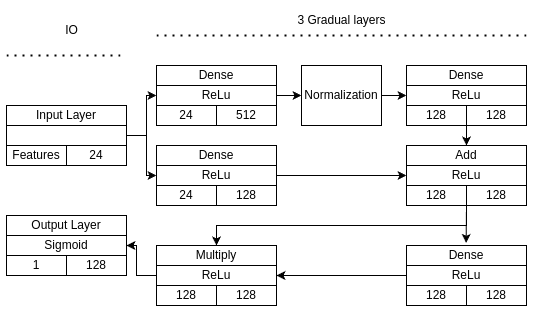
\includegraphics[width=0.8\textwidth]{obrazky-figures/tls_attention.png}
\caption{Architektura specializovaného TLS klasifikátoru s~feature-wise gatingem.}
\label{fig:tls_classifier_architecture}
\end{figure}

\section*{Výsledky klasifikace}
\label{appendix:tls-results}

Model \texttt{attention\_tls} byl testován ve třetí fázi klasifikace samostatně pro phishingové a malware domény. Na validační datové sadě dosahoval velmi vysoké výkonnosti – přesnost, úplnost i F1 skóre se pohybovaly nad 95~\%, jak shrnuje tabulka~\ref{tab:attention_tls_results}.


\begin{table}[h!]
    \centering
        \begin{tabular}{|l|c|c|}
            \hline
            \textbf{Metrika} & \textbf{Phishing} & \textbf{Malware} \\
            \hline
            Přesnost klasifikace (Accuracy)& 0{,}9934 ± 1{,}4e-04 & 0{,}9896 ± 7{,}8e-05 \\
            Přesnost pozitivní třídy (Precision)    & 0{,}9882 ± 8{,}8e-05 & 0{,}9660 ± 7{,}2e-05 \\
            Úplnost (Recall)        & 0{,}9722 ± 5{,}2e-05 & 0{,}9383 ± 5{,}7e-05 \\
            F1 skóre                & 0{,}9801 ± 6{,}4e-05 & 0{,}9519 ± 4{,}8e-05 \\
            ROC AUC                 & 0{,}9849 ± 7{,}9e-05 & 0{,}9671 ± 6{,}1e-05 \\
            \hline
        \end{tabular}
        \caption{Výsledky klasifikace modelu \texttt{tls} pro phishing a malware domény (10 běhů)}
    \label{tab:attention_tls_results}
\end{table}

Z~těchto výsledků vyplývá, že samotné TLS příznaky poskytují dostatečně bohatou informační hodnotu pro účinnou detekci škodlivých domén. Model vykazoval velmi vysoké hodnoty přesnosti, F1 skóre i AUC pro obě klasifikační úlohy a jeví se jako vhodný například pro nasazení v~prostředích s~omezeným přístupem k~DNS nebo aplikačním datům. Výsledky byly dále ověřeny na oddělené verifikační datové sadě, viz sekce \ref{verification_fail}.

\section*{Analýza matic záměn}

Kvalitu klasifikace potvrzuje i rozložení záměn zobrazené na obrázcích~\ref{fig:attention_tls_conf_matrix_phishing} a~\ref{fig:attention_tls_conf_matrix_malware}, kde je patrné minimum falešných pozitivních i negativních detekcí.

\begin{figure}[H]
    \centering
    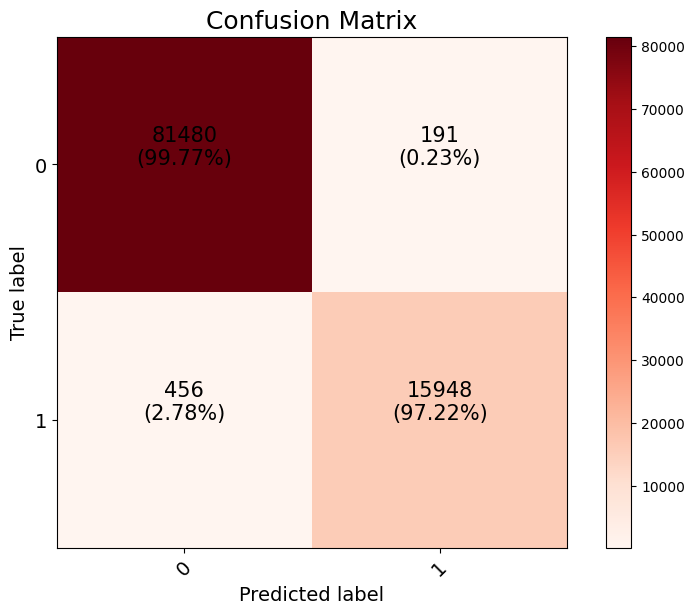
\includegraphics[width=0.8\textwidth]{obrazky-figures/attention_tls_stage_3_phishing_v1.1_confusion_matrix.png}
    \caption{Matice záměn pro phishingové domény (fáze~3).}
    \label{fig:attention_tls_conf_matrix_phishing}
\end{figure}

\begin{figure}[H]
    \centering
    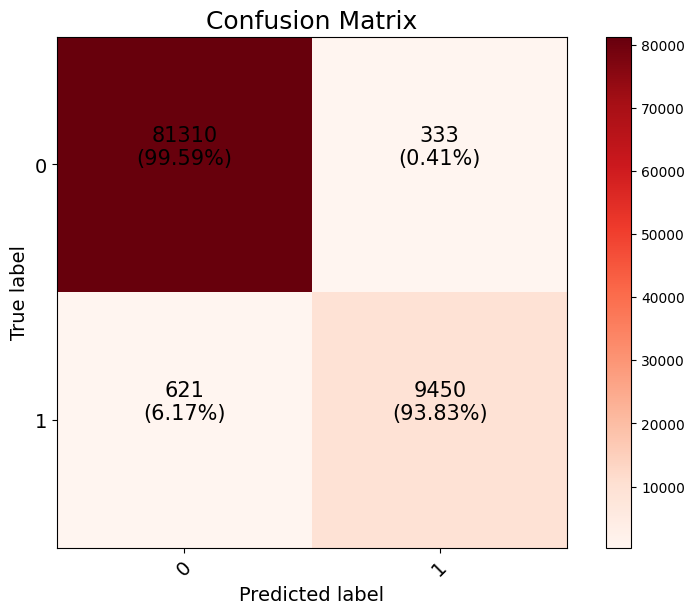
\includegraphics[width=0.8\textwidth]{obrazky-figures/attention_tls_stage_3_malware_v1.1_confusion_matrix.png}
    \caption{Matice záměn pro malware domény (fáze~3).}
    \label{fig:attention_tls_conf_matrix_malware}
\end{figure}

\section*{Výsledky na verifikační datové sadě}
\label{verification_fail}
Přestože model \texttt{attention\_tls} dosáhl velmi dobrých výsledků na validační datové sadě (viz Tabulka~\ref{tab:attention_tls_results}), jeho výkon na verifikačním vzorku byl výrazně slabší (viz Tabulka~\ref{tab:tls_attention_combined}) , zejména v~případě detekce malware domén. Zatímco recall zůstal vysoký, přesnost (precision) se u~obou úloh propadla, což naznačuje zvýšený počet falešně pozitivních klasifikací.

Z~důvodu této slabší generalizace nebyl model založený výhradně na TLS příznacích zapojen do výsledné klasifikační pipeline. Přesto však považujeme tento přístup za zajímavý směr dalšího výzkumu – zejména s~ohledem na nízké nároky na vstupní data a možnost jeho nasazení v~prostředích s~omezenými možnostmi hlubší inspekce.

\begin{table}[h!]
\centering
\begin{tabular}{|l|c|c|}
\hline
\textbf{Metrika} & \textbf{Malware} & \textbf{Phishing} \\
\hline
Přesnost klasifikace (Accuracy)      & \texttt{0.8750 ± 6.2e-05} & \texttt{0.9278 ± 4.8e-05} \\
Přesnost pozitivní třídy (Precision) & \texttt{0.5814 ± 1.1e-04} & \texttt{0.7072 ± 9.1e-05} \\
Úplnost (Recall)                     & \texttt{0.8117 ± 9.0e-05} & \texttt{0.9481 ± 9.3e-05} \\
F1 skóre                             & \texttt{0.6767 ± 5.8e-05} & \texttt{0.8101 ± 4.1e-05} \\
ROC AUC                              & \texttt{0.8573 ± 7.2e-05} & \texttt{0.9360 ± 7.0e-05} \\
\hline
\end{tabular}
\caption{Srovnání metrik modelu \texttt{attention\_tls} (Stage 3) pro malware a phishing (10 běhů).}
\label{tab:tls_attention_combined}
\end{table}

\section*{Závěr}

Specializovaný model \texttt{attention\_tls} ukázal, že je možné klasifikovat domény pouze na základě TLS metadat, bez nutnosti využití DNS, WHOIS nebo aplikačních příznaků. Při validaci dosáhl velmi dobrých výsledků a potvrdil, že TLS příznaky představují zajímavý, byť v~praxi dosud málo využívaný, zdroj informací pro detekci škodlivých domén.

Při testování na verifikační datové sadě se však ukázalo, že model nedosahuje stejné úrovně generalizace. Zatímco úplnost zůstala vysoká, přesnost poklesla, zejména v~případě malware domén, což vedlo ke zvýšenému výskytu falešně pozitivních klasifikací. Vzhledem k~těmto výsledkům nebyl model \texttt{attention\_tls} zařazen do finální klasifikační pipeline.

Přesto zůstává přístup založený na TLS a jeho samostatná klasifikace relevantní a slibnou oblastí pro další výzkum – zejména v~kontextu pasivního monitoringu, analýzy šifrovaného provozu a nasazení v~edge prostředích. Dále by bylo vhodné zkoumat možnosti rozšíření sady příznaků, robustnější trénovací přístupy a metody kombinace s~jinými modalitami pro zvýšení odolnosti vůči rozdílům v~distribuci dat mezi sadami.






\chapter{Výsledky analýzy SHAP}
\label{sec:appendix-shap}

Analýza Shapleyho hodnot (SHAP) poskytuje hlubší pohled na to, jak jednotlivé příznaky přispívají k~rozhodování konkrétních modelů. Následující grafy znázorňují distribuci hodnot SHAP pro každý model zvlášť.

\begin{figure}[!ht]
    \centering
    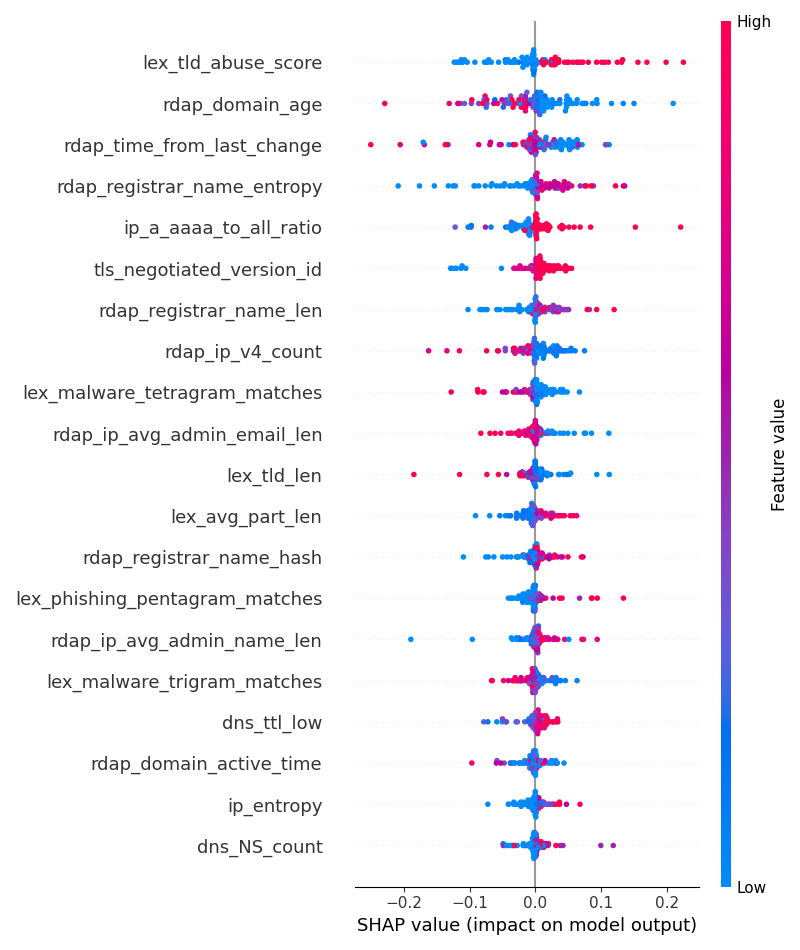
\includegraphics[width=1.0\textwidth]{obrazky-figures/shap_feedforward.png}
    \caption{Přínos jednotlivých příznaků pro model FFNN}
    \label{fig:shap_feedforward}
\end{figure}

Model FFNN klade největší důraz na příznaky z~oblasti RDAP  \texttt{rdap\_domain\_age}) a lexikálních znaků domény (např. \texttt{lex\_tld\_abuse\_score}). Dále je patrný vliv vybraných TLS atributů, i když jejich dopad je ve srovnání s~ostatními kategoriemi menší.

\begin{figure}[!ht]
    \centering
    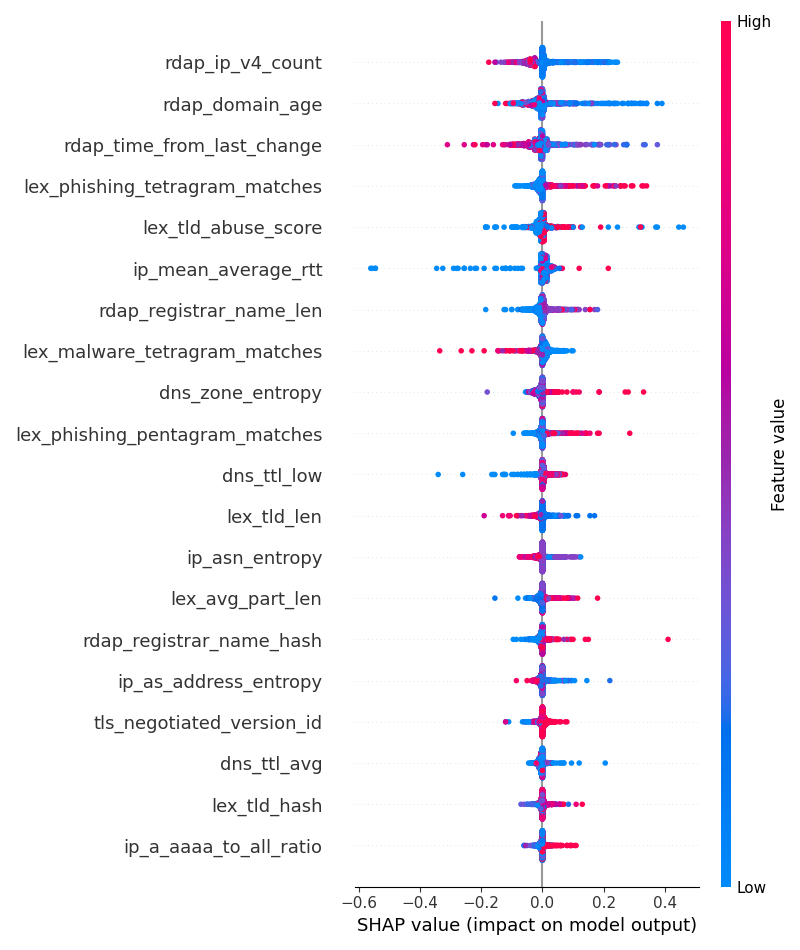
\includegraphics[width=1.0\textwidth]{obrazky-figures/shap_Lgbm.png}
    \caption{Přínos jednotlivých příznaků pro model LightGBM}
    \label{fig:shap_Lgbm}
\end{figure}

U~modelu LightGBM dominují atributy z~RDAP oblasti a DNS záznamy, přičemž příznak \texttt{rdap\_ip\_v4\_count} patří mezi nejvýznamnější. Rovněž se zde více uplatňuje informační entropie z~IP a DNS zón.

\begin{figure}[!ht]
    \centering
    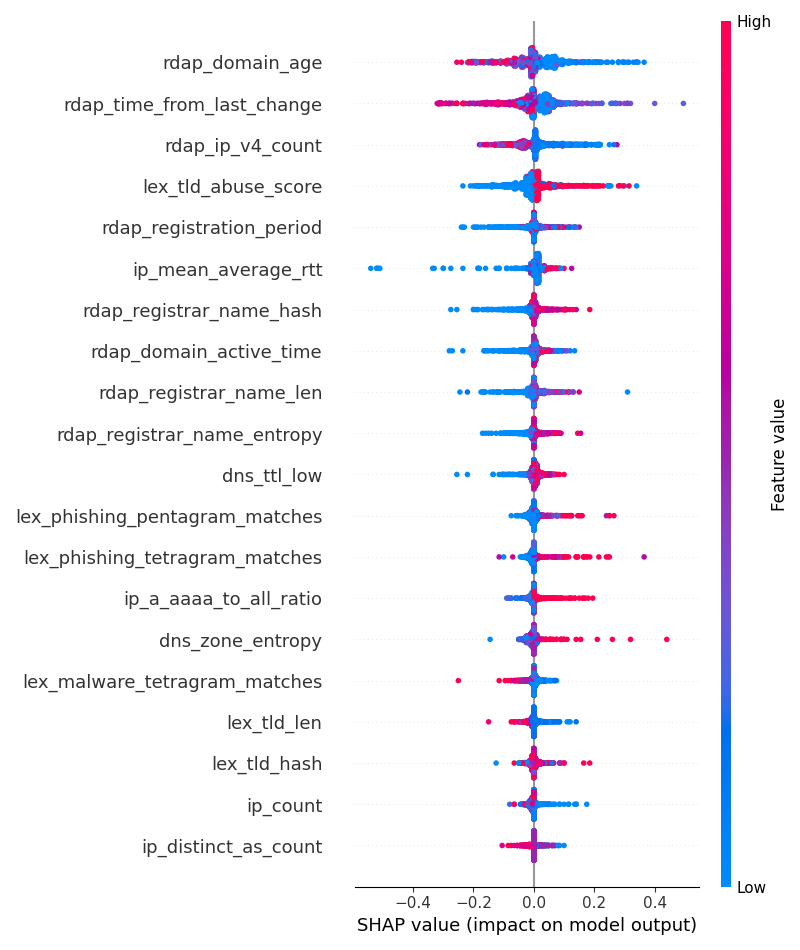
\includegraphics[width=1.0\textwidth]{obrazky-figures/shap_XgBoost.png}
    \caption{Přínos jednotlivých příznaků pro model XGBoost}
    \label{fig:shap_XgBoost}
\end{figure}

Model XGBoost se opírá o~podobné sady příznaků, nicméně více zvýrazňuje lexikální znaky druhé úrovně domény (např. \texttt{lex\_sld\_digit\_count}) a specifické TLS vlastnosti jako \texttt{tls\_CA\_certs\_in\_chain\_ratio}. Příznaky z~RDAP oblasti zůstávají důležitým základem.

\begin{figure}[!ht]
    \centering
    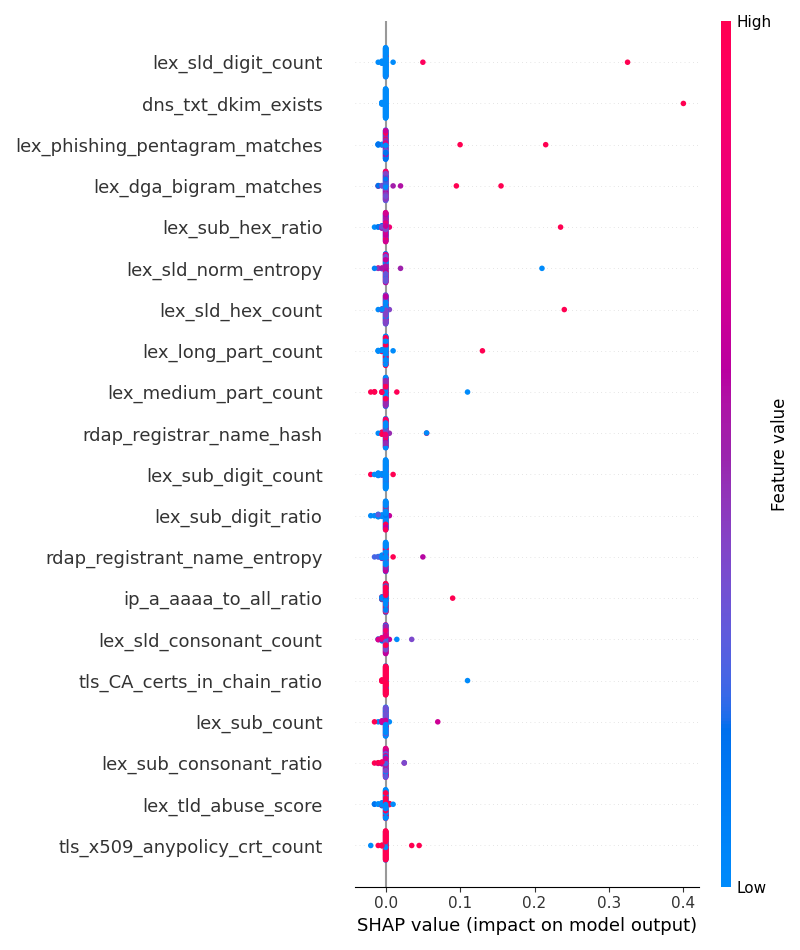
\includegraphics[width=1.0\textwidth]{obrazky-figures/shap_svm.png}
    \caption{Přínos jednotlivých příznaků pro model SVM}
    \label{fig:shap_svm}
\end{figure}

SVM model rovněž ukazuje silnou závislost na RDAP příznacích (věk domény, délka registrace), doplněnou o~lexikální charakteristiky a síťové vlastnosti. Model reflektuje robustní schopnost klasifikace při kombinaci více typů příznaků.

\section*{Přínos všech příznaků napříč modely}

Kromě pohledu na jednotlivé modely byla provedena agregovaná analýza SHAP hodnot napříč celou klasifikační pipeline.

\begin{figure}[!ht]
    \centering
    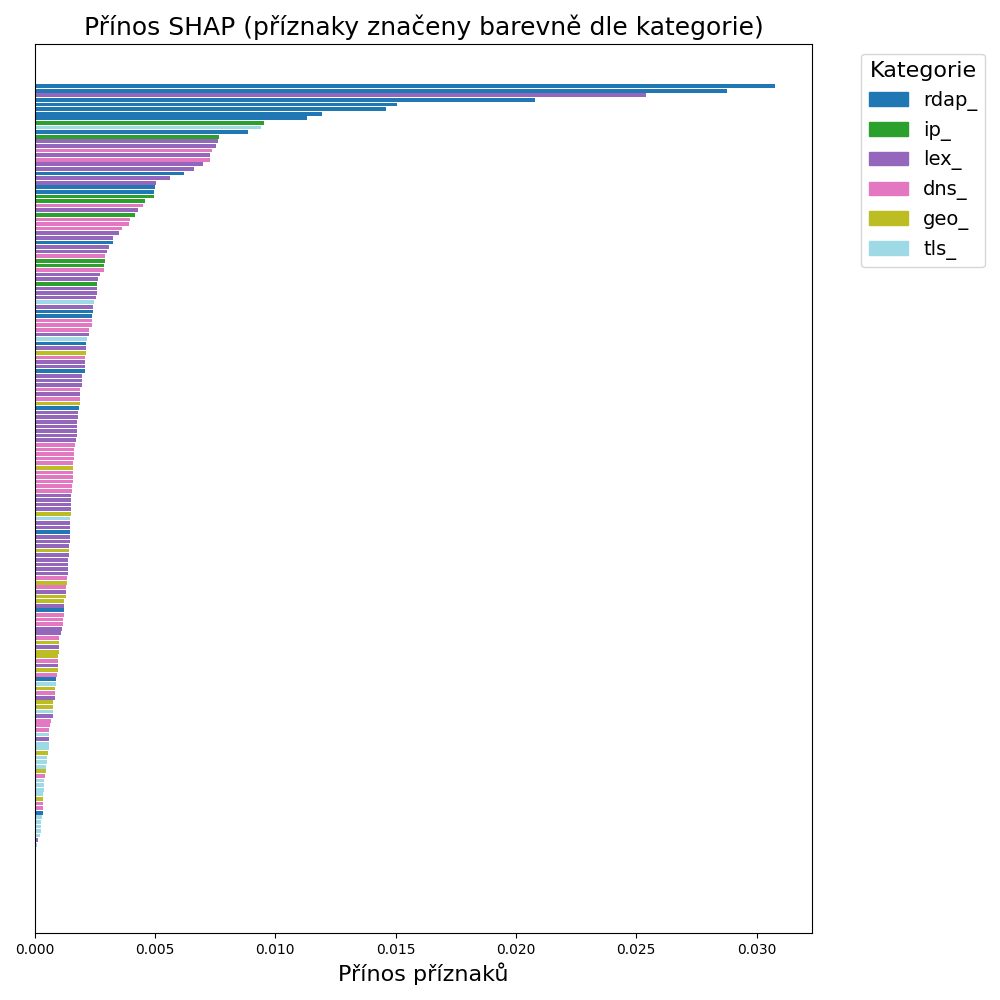
\includegraphics[width=1.0\textwidth]{obrazky-figures/all_shap.png}
    \caption{Průměrný SHAP přínos všech příznaků, barevně rozlišen dle kategorií}
    \label{fig:all_shap}
\end{figure}

Na obrázku \ref{fig:all_shap} jsou jednotlivé příznaky seřazeny dle jejich průměrného přínosu k~rozhodování. Dominují především příznaky z~RDAP oblasti, následované IP a lexikálními znaky. Barevné označení umožňuje sledovat, které kategorie přispívají nejvíce, a zároveň ukazuje značný pokles důležitosti u~DNS, GEO a TLS příznaků.

\begin{figure}[!ht]
    \centering
    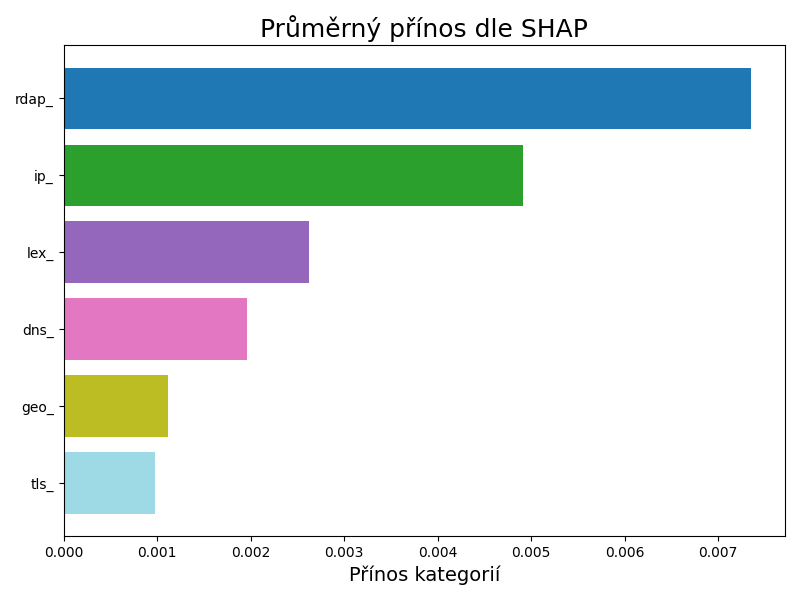
\includegraphics[width=0.8\textwidth]{obrazky-figures/shap_cat.png}
    \caption{Průměrný přínos příznaků dle kategorií}
    \label{fig:shap_cat}
\end{figure}

Konečný souhrn na obrázku \ref{fig:shap_cat} kvantifikuje průměrný přínos jednotlivých kategorií. Nejvyšší přínos vykazují RDAP příznaky, následované IP a lexikálními znaky domény. Naopak TLS a GEO atributy měly relativně nízký vliv, což naznačuje jejich omezenou roli v~celkové klasifikaci. Tyto poznatky mohou být vodítkem pro budoucí redukci dimenze nebo návrh specializovaných klasifikátorů pro jednotlivé kategorie.










\chapter{Měření klasifikace dle podmnožin}
\label{sec:appendix-results}

Tato příloha obsahuje kompletní výsledky všech měření samostatných i agregovaných subsetů příznaků pro klasifikaci phishingových a malware domén.

Každý výstup zobrazuje přesnost jednotlivých klasifikačních algoritmů na dané kombinaci příznaků, zvlášť pro phishing a zvlášť pro malware. Měření byla provedena podle metodologie popsané v~kapitole \textbf{Předběžná analýza podmnožin příznaků}, kde byl popsán postup automatizovaného trénování modelů pomocí knihovny \texttt{PyCaret}. Cílem bylo identifikovat optimální kombinace atributů a klasifikátorů pro detekci škodlivých domén.

\subsection*{Použité klasifikátory}

Následující tabulka obsahuje zkratky používané v~jednotlivých výstupech a jejich odpovídající plné názvy modelů. Tyto zkratky byly zvoleny pro zajištění přehlednosti a úsporu místa ve výstupech.

\begin{table}[H]
    \centering
    \caption{Zkratky použitých klasifikátorů}
    \label{tab:model_abbreviations}
    \begin{tabular}{|l|l|l|}
        \hline
        \textbf{Zkratka} & \textbf{Plný název} & \textbf{Poznámka} \\
        \hline
        \texttt{RF} & Random Forest Classifier & Ensemble \\
        \texttt{ADA} & Ada Boost Classifier & Ensemble \\
        \texttt{DT} & Decision Tree Classifier & Interpretable \\
        \texttt{Ridge} & Ridge Classifier & Linear model \\
        \texttt{KNN} & K~Neighbors Classifier & Instance-based \\
        \texttt{SVM-L} & SVM - Linear Kernel & Linear SVM \\
        \texttt{LR} & Logistic Regression & Linear model \\
        \texttt{QDA} & Quadratic Discriminant Analysis & Probabilistic \\
        \texttt{NB} & Naive Bayes & Probabilistic \\
        \texttt{ET} & Extra Trees Classifier & Ensemble \\
        \texttt{XGB} & Extreme Gradient Boosting & Boosted Trees \\
        \texttt{LGBM} & Light Gradient Boosting Machine & Boosted Trees \\
        \texttt{GBC} & Gradient Boosting Classifier & Boosted Trees \\
        \texttt{LDA} & Linear Discriminant Analysis & Probabilistic \\
        \texttt{Dummy} & Dummy Classifier & Referenční baseline \\
        \hline
    \end{tabular}
\end{table}

\subsection*{Komentář k~výstupům}

Každá tabulka představuje výsledky pro konkrétní subset příznaků a typ útoku (phishing nebo malware).  
Metody jsou porovnávány dle hlavních metrik klasifikace: přesnost (\textbf{Acc}), plocha pod ROC křivkou (\textbf{AUC}), \textbf{Recall}, \textbf{Precision}, \textbf{F1 skóre}, Cohenova \textbf{Kappa} a \textbf{Matthews Correlation Coefficient} (MCC).

Díky oddělení výsledků pro phishing a malware je možné detailně porovnat účinnost jednotlivých přístupů pro různé typy útoků a rozhodnout o~vhodné strategii nasazení.

\bigskip

\begin{table}[H]
  \centering
  \small
  \caption{Výsledky pro subset dns – malware}
  \begin{tabular}{|l|c|c|c|c|c|c|c|c|}
    \hline
    \textbf{Model} & \textbf{Acc} & \textbf{AUC} & \textbf{Recall} & \textbf{Prec.} & \textbf{F1} & \textbf{Kappa} & \textbf{MCC} & \textbf{TT (s)} \\
    \hline
    Random Forest Classifier & 0.9165 & 0.9120 & 0.9165 & 0.9135 & 0.9143 & 0.6861 & 0.6886 & 1.80 \\
    Extra Trees Classifier & 0.9155 & 0.8910 & 0.9155 & 0.9125 & 0.9133 & 0.6829 & 0.6851 & 0.45 \\
    K Neighbors Classifier & 0.9142 & 0.8860 & 0.9142 & 0.9109 & 0.9116 & 0.6757 & 0.6787 & 0.24 \\
    Extreme Gradient Boosting & 0.9166 & 0.9175 & 0.9166 & 0.9129 & 0.9115 & 0.6681 & 0.6785 & 0.44 \\
    Light Gradient Boosting Machine & 0.9174 & 0.9176 & 0.9174 & 0.9144 & 0.9113 & 0.6647 & 0.6794 & 0.61 \\
    Decision Tree Classifier & 0.8958 & 0.8503 & 0.8958 & 0.8957 & 0.8957 & 0.6268 & 0.6271 & 0.19 \\
    Gradient Boosting Classifier & 0.8911 & 0.8799 & 0.8911 & 0.8921 & 0.8728 & 0.4991 & 0.5538 & 2.77 \\
    Ada Boost Classifier & 0.8632 & 0.8417 & 0.8632 & 0.8536 & 0.8335 & 0.3352 & 0.3997 & 0.71 \\
    Linear Discriminant Analysis & 0.8491 & 0.7843 & 0.8491 & 0.8264 & 0.8136 & 0.2532 & 0.3100 & 0.17 \\
    Ridge Classifier & 0.8346 & 0.7842 & 0.8346 & 0.7962 & 0.7724 & 0.0722 & 0.1401 & 0.12 \\
    Logistic Regression & 0.8242 & 0.6988 & 0.8242 & 0.7307 & 0.7582 & 0.0143 & 0.0262 & 1.31 \\
    Dummy Classifier & 0.8317 & 0.5000 & 0.8317 & 0.6917 & 0.7553 & 0.0000 & 0.0000 & 0.06 \\
    SVM - Linear Kernel & 0.6466 & 0.6454 & 0.6466 & 0.7720 & 0.6756 & 0.1180 & 0.1475 & 0.14 \\
    Quadratic Discriminant Analysis & 0.5847 & 0.7880 & 0.5847 & 0.8468 & 0.6332 & 0.2208 & 0.3161 & 0.14 \\
    Naive Bayes & 0.3432 & 0.6313 & 0.3432 & 0.8202 & 0.3546 & 0.0640 & 0.1513 & 0.07 \\
    \hline
  \end{tabular}
\end{table}
\vspace{0.5cm}

\begin{table}[H]
  \centering
  \small
  \caption{Výsledky pro subset geo – malware}
  \begin{tabular}{|l|c|c|c|c|c|c|c|c|}
    \hline
    \textbf{Model} & \textbf{Acc} & \textbf{AUC} & \textbf{Recall} & \textbf{Prec.} & \textbf{F1} & \textbf{Kappa} & \textbf{MCC} & \textbf{TT (s)} \\
    \hline
    Random Forest Classifier & 0.8461 & 0.8194 & 0.8461 & 0.8210 & 0.8106 & 0.2416 & 0.2948 & 0.28 \\
    Extra Trees Classifier & 0.8461 & 0.8173 & 0.8461 & 0.8210 & 0.8102 & 0.2400 & 0.2939 & 0.25 \\
    Light Gradient Boosting Machine & 0.8482 & 0.8291 & 0.8482 & 0.8272 & 0.8098 & 0.2352 & 0.2998 & 0.62 \\
    Decision Tree Classifier & 0.8446 & 0.8161 & 0.8446 & 0.8176 & 0.8092 & 0.2367 & 0.2870 & 0.13 \\
    Extreme Gradient Boosting & 0.8474 & 0.8277 & 0.8474 & 0.8249 & 0.8092 & 0.2333 & 0.2953 & 0.22 \\
    K Neighbors Classifier & 0.8380 & 0.7701 & 0.8380 & 0.8056 & 0.8031 & 0.2147 & 0.2555 & 0.15 \\
    Gradient Boosting Classifier & 0.8446 & 0.8170 & 0.8446 & 0.8218 & 0.8000 & 0.1915 & 0.2634 & 2.24 \\
    Ada Boost Classifier & 0.8342 & 0.7980 & 0.8342 & 0.7815 & 0.7674 & 0.0511 & 0.1055 & 0.63 \\
    Ridge Classifier & 0.8317 & 0.6927 & 0.8317 & 0.6917 & 0.7553 & -0.0001 & -0.0010 & 0.10 \\
    Linear Discriminant Analysis & 0.8317 & 0.6928 & 0.8317 & 0.6917 & 0.7553 & -0.0001 & -0.0010 & 0.13 \\
    Dummy Classifier & 0.8317 & 0.5000 & 0.8317 & 0.6917 & 0.7553 & 0.0000 & 0.0000 & 0.06 \\
    Logistic Regression & 0.8311 & 0.7075 & 0.8311 & 0.7085 & 0.7551 & -0.0008 & -0.0044 & 1.28 \\
    SVM - Linear Kernel & 0.7870 & 0.5542 & 0.7870 & 0.7089 & 0.7393 & 0.0064 & 0.0019 & 0.13 \\
    Quadratic Discriminant Analysis & 0.4123 & 0.7363 & 0.4123 & 0.8469 & 0.4425 & 0.1110 & 0.2242 & 0.11 \\
    Naive Bayes & 0.3427 & 0.6407 & 0.3427 & 0.7833 & 0.3620 & 0.0453 & 0.1011 & 0.06 \\
    \hline
  \end{tabular}
\end{table}
\vspace{0.5cm}

\begin{table}[H]
  \centering
  \small
  \caption{Výsledky pro subset html – malware}
  \begin{tabular}{|l|c|c|c|c|c|c|c|c|}
    \hline
    \textbf{Model} & \textbf{Acc} & \textbf{AUC} & \textbf{Recall} & \textbf{Prec.} & \textbf{F1} & \textbf{Kappa} & \textbf{MCC} & \textbf{TT (s)} \\
    \hline
    Random Forest Classifier & 0.8410 & 0.7060 & 0.8410 & 0.8313 & 0.7824 & 0.1133 & 0.2110 & 0.38 \\
    Light Gradient Boosting Machine & 0.8414 & 0.7098 & 0.8414 & 0.8357 & 0.7823 & 0.1127 & 0.2145 & 1.20 \\
    Extreme Gradient Boosting & 0.8411 & 0.7090 & 0.8411 & 0.8327 & 0.7822 & 0.1125 & 0.2115 & 0.34 \\
    Extra Trees Classifier & 0.8403 & 0.7009 & 0.8403 & 0.8260 & 0.7820 & 0.1117 & 0.2046 & 0.31 \\
    K Neighbors Classifier & 0.8409 & 0.6828 & 0.8409 & 0.8346 & 0.7811 & 0.1075 & 0.2087 & 0.21 \\
    Gradient Boosting Classifier & 0.8416 & 0.7078 & 0.8416 & 0.8485 & 0.7804 & 0.1041 & 0.2174 & 4.35 \\
    Ada Boost Classifier & 0.8411 & 0.6954 & 0.8411 & 0.8476 & 0.7793 & 0.0995 & 0.2111 & 1.20 \\
    Decision Tree Classifier & 0.8285 & 0.6875 & 0.8285 & 0.7733 & 0.7745 & 0.0854 & 0.1272 & 0.28 \\
    Logistic Regression & 0.8313 & 0.6499 & 0.8313 & 0.7142 & 0.7553 & -0.0000 & 0.0011 & 1.73 \\
    Dummy Classifier & 0.8317 & 0.5000 & 0.8317 & 0.6917 & 0.7553 & 0.0000 & 0.0000 & 0.08 \\
    Ridge Classifier & 0.8315 & 0.6633 & 0.8315 & 0.6917 & 0.7552 & -0.0004 & -0.0034 & 0.16 \\
    Linear Discriminant Analysis & 0.8314 & 0.6617 & 0.8314 & 0.6917 & 0.7551 & -0.0007 & -0.0063 & 0.29 \\
    SVM - Linear Kernel & 0.7869 & 0.6562 & 0.7869 & 0.7278 & 0.7350 & 0.0172 & 0.0288 & 0.24 \\
    Naive Bayes & 0.4640 & 0.6623 & 0.4640 & 0.8337 & 0.5074 & 0.1309 & 0.2305 & 0.09 \\
    Quadratic Discriminant Analysis & 0.4459 & 0.6664 & 0.4459 & 0.8477 & 0.4837 & 0.1304 & 0.2437 & 0.20 \\
    \hline
  \end{tabular}
\end{table}
\vspace{0.5cm}

\begin{table}[H]
  \centering
  \small
  \caption{Výsledky pro subset ip – malware}
  \begin{tabular}{|l|c|c|c|c|c|c|c|c|}
    \hline
    \textbf{Model} & \textbf{Acc} & \textbf{AUC} & \textbf{Recall} & \textbf{Prec.} & \textbf{F1} & \textbf{Kappa} & \textbf{MCC} & \textbf{TT (s)} \\
    \hline
    Extreme Gradient Boosting & 0.8669 & 0.8812 & 0.8669 & 0.8524 & 0.8511 & 0.4242 & 0.4478 & 0.22 \\
    Light Gradient Boosting Machine & 0.8669 & 0.8817 & 0.8669 & 0.8524 & 0.8490 & 0.4124 & 0.4414 & 0.59 \\
    K Neighbors Classifier & 0.8553 & 0.8210 & 0.8553 & 0.8452 & 0.8469 & 0.4289 & 0.4379 & 0.20 \\
    Random Forest Classifier & 0.8437 & 0.8314 & 0.8437 & 0.8312 & 0.8359 & 0.3888 & 0.3930 & 0.32 \\
    Extra Trees Classifier & 0.8425 & 0.7755 & 0.8425 & 0.8296 & 0.8343 & 0.3824 & 0.3868 & 0.35 \\
    Gradient Boosting Classifier & 0.8589 & 0.8582 & 0.8589 & 0.8421 & 0.8326 & 0.3372 & 0.3833 & 1.13 \\
    Decision Tree Classifier & 0.8406 & 0.7284 & 0.8406 & 0.8273 & 0.8322 & 0.3740 & 0.3786 & 0.10 \\
    Ada Boost Classifier & 0.8404 & 0.8359 & 0.8404 & 0.8126 & 0.7911 & 0.1533 & 0.2249 & 0.39 \\
    Linear Discriminant Analysis & 0.8317 & 0.7536 & 0.8317 & 0.7283 & 0.7556 & 0.0015 & 0.0107 & 0.12 \\
    Ridge Classifier & 0.8317 & 0.7537 & 0.8317 & 0.6917 & 0.7553 & -0.0001 & -0.0010 & 0.10 \\
    Dummy Classifier & 0.8317 & 0.5000 & 0.8317 & 0.6917 & 0.7553 & 0.0000 & 0.0000 & 0.06 \\
    Logistic Regression & 0.8306 & 0.7597 & 0.8306 & 0.7085 & 0.7551 & -0.0007 & -0.0047 & 0.38 \\
    SVM - Linear Kernel & 0.7730 & 0.6588 & 0.7730 & 0.7781 & 0.7467 & 0.1158 & 0.1512 & 0.18 \\
    Quadratic Discriminant Analysis & 0.5441 & 0.7503 & 0.5441 & 0.8516 & 0.5921 & 0.1961 & 0.3035 & 0.10 \\
    Naive Bayes & 0.5152 & 0.6785 & 0.5152 & 0.8361 & 0.5638 & 0.1630 & 0.2599 & 0.06 \\
    \hline
  \end{tabular}
\end{table}
\vspace{0.5cm}

\begin{table}[H]
  \centering
  \small
  \caption{Výsledky pro subset lex – malware}
  \begin{tabular}{|l|c|c|c|c|c|c|c|c|}
    \hline
    \textbf{Model} & \textbf{Acc} & \textbf{AUC} & \textbf{Recall} & \textbf{Prec.} & \textbf{F1} & \textbf{Kappa} & \textbf{MCC} & \textbf{TT (s)} \\
    \hline
    Light Gradient Boosting Machine & 0.9371 & 0.9352 & 0.9371 & 0.9358 & 0.9338 & 0.7531 & 0.7618 & 0.69 \\
    Extreme Gradient Boosting & 0.9341 & 0.9303 & 0.9341 & 0.9321 & 0.9311 & 0.7441 & 0.7507 & 0.33 \\
    Gradient Boosting Classifier & 0.9255 & 0.9204 & 0.9255 & 0.9248 & 0.9194 & 0.6940 & 0.7125 & 5.58 \\
    Random Forest Classifier & 0.9238 & 0.9144 & 0.9238 & 0.9215 & 0.9188 & 0.6944 & 0.7068 & 0.44 \\
    Extra Trees Classifier & 0.9213 & 0.8860 & 0.9213 & 0.9187 & 0.9158 & 0.6824 & 0.6959 & 0.50 \\
    Ada Boost Classifier & 0.9066 & 0.8994 & 0.9066 & 0.9018 & 0.8989 & 0.6161 & 0.6325 & 1.28 \\
    Linear Discriminant Analysis & 0.8987 & 0.8850 & 0.8987 & 0.8952 & 0.8864 & 0.5604 & 0.5920 & 0.23 \\
    Decision Tree Classifier & 0.8761 & 0.7909 & 0.8761 & 0.8780 & 0.8769 & 0.5637 & 0.5639 & 0.38 \\
    Ridge Classifier & 0.8929 & 0.8852 & 0.8929 & 0.8945 & 0.8751 & 0.5083 & 0.5627 & 0.12 \\
    K Neighbors Classifier & 0.8635 & 0.7860 & 0.8635 & 0.8479 & 0.8475 & 0.4106 & 0.4329 & 0.20 \\
    Logistic Regression & 0.8317 & 0.4768 & 0.8317 & 0.6917 & 0.7553 & 0.0000 & 0.0000 & 0.17 \\
    Naive Bayes & 0.8317 & 0.5302 & 0.8317 & 0.6917 & 0.7553 & 0.0000 & 0.0000 & 0.08 \\
    SVM - Linear Kernel & 0.8317 & 0.4927 & 0.8317 & 0.6917 & 0.7553 & 0.0000 & 0.0000 & 0.63 \\
    Dummy Classifier & 0.8317 & 0.5000 & 0.8317 & 0.6917 & 0.7553 & 0.0000 & 0.0000 & 0.07 \\
    Quadratic Discriminant Analysis & 0.3245 & 0.8671 & 0.3245 & 0.8487 & 0.3192 & 0.0676 & 0.1740 & 0.15 \\
    \hline
  \end{tabular}
\end{table}
\vspace{0.5cm}

\begin{table}[H]
  \centering
  \small
  \caption{Výsledky pro subset rdap – malware}
  \begin{tabular}{|l|c|c|c|c|c|c|c|c|}
    \hline
    \textbf{Model} & \textbf{Acc} & \textbf{AUC} & \textbf{Recall} & \textbf{Prec.} & \textbf{F1} & \textbf{Kappa} & \textbf{MCC} & \textbf{TT (s)} \\
    \hline
    Light Gradient Boosting Machine & 0.9533 & 0.9590 & 0.9533 & 0.9524 & 0.9518 & 0.8228 & 0.8265 & 0.64 \\
    Extreme Gradient Boosting & 0.9522 & 0.9589 & 0.9522 & 0.9512 & 0.9509 & 0.8204 & 0.8230 & 0.35 \\
    Random Forest Classifier & 0.9502 & 0.9572 & 0.9502 & 0.9491 & 0.9487 & 0.8121 & 0.8151 & 0.33 \\
    Extra Trees Classifier & 0.9467 & 0.9410 & 0.9467 & 0.9455 & 0.9450 & 0.7980 & 0.8016 & 0.33 \\
    Gradient Boosting Classifier & 0.9358 & 0.9420 & 0.9358 & 0.9342 & 0.9326 & 0.7489 & 0.7568 & 3.20 \\
    Decision Tree Classifier & 0.9319 & 0.8981 & 0.9319 & 0.9313 & 0.9315 & 0.7541 & 0.7543 & 0.19 \\
    K Neighbors Classifier & 0.9296 & 0.8997 & 0.9296 & 0.9275 & 0.9281 & 0.7381 & 0.7396 & 0.17 \\
    Ada Boost Classifier & 0.9196 & 0.9229 & 0.9196 & 0.9160 & 0.9159 & 0.6877 & 0.6938 & 0.81 \\
    Linear Discriminant Analysis & 0.8576 & 0.8538 & 0.8576 & 0.8402 & 0.8421 & 0.3919 & 0.4102 & 0.14 \\
    Ridge Classifier & 0.8476 & 0.8539 & 0.8476 & 0.8271 & 0.8067 & 0.2207 & 0.2905 & 0.11 \\
    Naive Bayes & 0.8317 & 0.7152 & 0.8317 & 0.6917 & 0.7553 & 0.0000 & 0.0000 & 0.07 \\
    Dummy Classifier & 0.8317 & 0.5000 & 0.8317 & 0.6917 & 0.7553 & 0.0000 & 0.0000 & 0.06 \\
    Logistic Regression & 0.6944 & 0.4346 & 0.6944 & 0.6868 & 0.6857 & -0.0985 & -0.1081 & 0.16 \\
    Quadratic Discriminant Analysis & 0.6038 & 0.8827 & 0.6038 & 0.8596 & 0.6506 & 0.2492 & 0.3524 & 0.12 \\
    SVM - Linear Kernel & 0.4393 & 0.4665 & 0.4393 & 0.6703 & 0.4658 & -0.1430 & -0.1609 & 0.36 \\
    \hline
  \end{tabular}
\end{table}
\vspace{0.5cm}

\begin{table}[H]
  \centering
  \small
  \caption{Výsledky pro subset tls – malware}
  \begin{tabular}{|l|c|c|c|c|c|c|c|c|}
    \hline
    \textbf{Model} & \textbf{Acc} & \textbf{AUC} & \textbf{Recall} & \textbf{Prec.} & \textbf{F1} & \textbf{Kappa} & \textbf{MCC} & \textbf{TT (s)} \\
    \hline
    Decision Tree Classifier & 0.8370 & 0.6894 & 0.8370 & 0.8323 & 0.7706 & 0.0633 & 0.1591 & 0.07 \\
    Random Forest Classifier & 0.8373 & 0.6889 & 0.8373 & 0.8393 & 0.7705 & 0.0629 & 0.1633 & 0.21 \\
    Extra Trees Classifier & 0.8371 & 0.6887 & 0.8371 & 0.8362 & 0.7705 & 0.0629 & 0.1612 & 0.23 \\
    Extreme Gradient Boosting & 0.8370 & 0.6919 & 0.8370 & 0.8360 & 0.7703 & 0.0620 & 0.1600 & 0.28 \\
    Light Gradient Boosting Machine & 0.8369 & 0.6885 & 0.8369 & 0.8346 & 0.7701 & 0.0613 & 0.1580 & 0.49 \\
    Gradient Boosting Classifier & 0.8366 & 0.6848 & 0.8366 & 0.8371 & 0.7689 & 0.0562 & 0.1531 & 0.56 \\
    Ada Boost Classifier & 0.8356 & 0.6326 & 0.8356 & 0.8327 & 0.7670 & 0.0482 & 0.1385 & 0.28 \\
    Ridge Classifier & 0.8349 & 0.6280 & 0.8349 & 0.8172 & 0.7667 & 0.0473 & 0.1275 & 0.12 \\
    Linear Discriminant Analysis & 0.8330 & 0.6279 & 0.8330 & 0.7916 & 0.7665 & 0.0469 & 0.1093 & 0.14 \\
    K Neighbors Classifier & 0.8342 & 0.5444 & 0.8342 & 0.8192 & 0.7641 & 0.0364 & 0.1129 & 0.15 \\
    Naive Bayes & 0.8280 & 0.5668 & 0.8280 & 0.7525 & 0.7608 & 0.0239 & 0.0522 & 0.06 \\
    Dummy Classifier & 0.8317 & 0.5000 & 0.8317 & 0.6917 & 0.7553 & 0.0000 & 0.0000 & 0.06 \\
    Logistic Regression & 0.7481 & 0.5816 & 0.7481 & 0.7399 & 0.7438 & 0.0706 & 0.0707 & 0.15 \\
    SVM - Linear Kernel & 0.6982 & 0.5314 & 0.6982 & 0.7315 & 0.6935 & 0.0594 & 0.0544 & 0.31 \\
    Quadratic Discriminant Analysis & 0.6663 & 0.5838 & 0.6663 & 0.7567 & 0.6503 & 0.0769 & 0.0889 & 0.12 \\
    \hline
  \end{tabular}
\end{table}
\vspace{0.5cm}

\begin{table}[H]
  \centering
  \small
  \caption{Výsledky pro subset dns+rdap+tls+geo+ip+html+lex – malware}
  \begin{tabular}{|l|c|c|c|c|c|c|c|c|}
    \hline
    \textbf{Model} & \textbf{Acc} & \textbf{AUC} & \textbf{Recall} & \textbf{Prec.} & \textbf{F1} & \textbf{Kappa} & \textbf{MCC} & \textbf{TT (s)} \\
    \hline
    Light Gradient Boosting Machine & 0.9975 & 0.9999 & 0.9975 & 0.9975 & 0.9975 & 0.9874 & 0.9874 & 1.90 \\
    Extreme Gradient Boosting & 0.9974 & 0.9999 & 0.9974 & 0.9974 & 0.9974 & 0.9868 & 0.9868 & 4.62 \\
    Gradient Boosting Classifier & 0.9951 & 0.9997 & 0.9951 & 0.9951 & 0.9951 & 0.9752 & 0.9752 & 62.63 \\
    Ada Boost Classifier & 0.9945 & 0.9996 & 0.9945 & 0.9945 & 0.9945 & 0.9719 & 0.9719 & 14.63 \\
    Random Forest Classifier & 0.9942 & 0.9996 & 0.9942 & 0.9942 & 0.9941 & 0.9697 & 0.9699 & 2.64 \\
    Decision Tree Classifier & 0.9930 & 0.9829 & 0.9930 & 0.9930 & 0.9930 & 0.9643 & 0.9644 & 1.43 \\
    Extra Trees Classifier & 0.9888 & 0.9985 & 0.9888 & 0.9888 & 0.9885 & 0.9402 & 0.9415 & 3.27 \\
    Linear Discriminant Analysis & 0.9817 & 0.9958 & 0.9817 & 0.9817 & 0.9817 & 0.9063 & 0.9063 & 2.40 \\
    Ridge Classifier & 0.9774 & 0.9958 & 0.9774 & 0.9770 & 0.9767 & 0.8775 & 0.8801 & 0.71 \\
    K Neighbors Classifier & 0.9530 & 0.9313 & 0.9530 & 0.9512 & 0.9517 & 0.7471 & 0.7488 & 2.13 \\
    Logistic Regression & 0.9265 & 0.9632 & 0.9265 & 0.9228 & 0.9242 & 0.6016 & 0.6035 & 16.57 \\
    Dummy Classifier & 0.8901 & 0.5000 & 0.8901 & 0.7923 & 0.8384 & 0.0000 & 0.0000 & 0.47 \\
    SVM - Linear Kernel & 0.8355 & 0.6441 & 0.8355 & 0.8080 & 0.8110 & 0.0235 & 0.0326 & 7.67 \\
    Quadratic Discriminant Analysis & 0.7671 & 0.9591 & 0.7671 & 0.9177 & 0.8090 & 0.3690 & 0.4622 & 1.91 \\
    Naive Bayes & 0.6445 & 0.9416 & 0.6445 & 0.9136 & 0.7097 & 0.2464 & 0.3704 & 0.69 \\
    \hline
  \end{tabular}
\end{table}
\vspace{0.5cm}

\begin{table}[H]
  \centering
  \small
  \caption{Výsledky pro subset dns+rdap – malware}
  \begin{tabular}{|l|c|c|c|c|c|c|c|c|}
    \hline
    \textbf{Model} & \textbf{Acc} & \textbf{AUC} & \textbf{Recall} & \textbf{Prec.} & \textbf{F1} & \textbf{Kappa} & \textbf{MCC} & \textbf{TT (s)} \\
    \hline
    Light Gradient Boosting Machine & 0.9897 & 0.9989 & 0.9897 & 0.9898 & 0.9897 & 0.9478 & 0.9478 & 0.87 \\
    Extreme Gradient Boosting & 0.9895 & 0.9989 & 0.9895 & 0.9895 & 0.9895 & 0.9465 & 0.9465 & 1.25 \\
    Random Forest Classifier & 0.9878 & 0.9973 & 0.9878 & 0.9877 & 0.9878 & 0.9370 & 0.9371 & 1.08 \\
    Extra Trees Classifier & 0.9847 & 0.9933 & 0.9847 & 0.9845 & 0.9844 & 0.9192 & 0.9200 & 1.01 \\
    Decision Tree Classifier & 0.9826 & 0.9564 & 0.9826 & 0.9827 & 0.9827 & 0.9114 & 0.9114 & 0.44 \\
    Gradient Boosting Classifier & 0.9825 & 0.9971 & 0.9825 & 0.9826 & 0.9826 & 0.9109 & 0.9109 & 18.98 \\
    Ada Boost Classifier & 0.9800 & 0.9965 & 0.9800 & 0.9803 & 0.9801 & 0.8989 & 0.8990 & 4.46 \\
    Linear Discriminant Analysis & 0.9519 & 0.9794 & 0.9519 & 0.9520 & 0.9519 & 0.7547 & 0.7547 & 0.69 \\
    K Neighbors Classifier & 0.9423 & 0.9239 & 0.9423 & 0.9404 & 0.9411 & 0.6933 & 0.6943 & 1.04 \\
    Ridge Classifier & 0.9407 & 0.9794 & 0.9407 & 0.9388 & 0.9334 & 0.6265 & 0.6562 & 0.35 \\
    Quadratic Discriminant Analysis & 0.8580 & 0.9716 & 0.8580 & 0.9339 & 0.8793 & 0.5287 & 0.5916 & 0.48 \\
    Logistic Regression & 0.8942 & 0.9420 & 0.8942 & 0.8710 & 0.8747 & 0.2767 & 0.3070 & 5.40 \\
    Dummy Classifier & 0.8901 & 0.5000 & 0.8901 & 0.7923 & 0.8384 & 0.0000 & 0.0000 & 0.21 \\
    SVM - Linear Kernel & 0.8407 & 0.5971 & 0.8407 & 0.8208 & 0.8149 & 0.0353 & 0.0527 & 2.73 \\
    Naive Bayes & 0.6356 & 0.9308 & 0.6356 & 0.9131 & 0.7022 & 0.2386 & 0.3638 & 0.27 \\
    \hline
  \end{tabular}
\end{table}
\vspace{0.5cm}

\begin{table}[H]
  \centering
  \small
  \caption{Výsledky pro subset dns – malware}
  \begin{tabular}{|l|c|c|c|c|c|c|c|c|}
    \hline
    \textbf{Model} & \textbf{Acc} & \textbf{AUC} & \textbf{Recall} & \textbf{Prec.} & \textbf{F1} & \textbf{Kappa} & \textbf{MCC} & \textbf{TT (s)} \\
    \hline
    Extreme Gradient Boosting & 0.9193 & 0.8869 & 0.9193 & 0.9110 & 0.9080 & 0.4945 & 0.5247 & 0.66 \\
    Random Forest Classifier & 0.9156 & 0.8698 & 0.9156 & 0.9059 & 0.9067 & 0.4961 & 0.5136 & 0.96 \\
    K Neighbors Classifier & 0.9133 & 0.8388 & 0.9133 & 0.9040 & 0.9060 & 0.4989 & 0.5103 & 0.39 \\
    Light Gradient Boosting Machine & 0.9197 & 0.8913 & 0.9197 & 0.9133 & 0.9059 & 0.4744 & 0.5193 & 0.74 \\
    Extra Trees Classifier & 0.9139 & 0.8390 & 0.9139 & 0.9042 & 0.9058 & 0.4952 & 0.5089 & 0.68 \\
    Gradient Boosting Classifier & 0.9084 & 0.8640 & 0.9084 & 0.8977 & 0.8888 & 0.3693 & 0.4255 & 5.49 \\
    Decision Tree Classifier & 0.8881 & 0.7566 & 0.8881 & 0.8838 & 0.8858 & 0.4206 & 0.4212 & 0.39 \\
    Ada Boost Classifier & 0.9037 & 0.8368 & 0.9037 & 0.8898 & 0.8824 & 0.3311 & 0.3864 & 1.36 \\
    Linear Discriminant Analysis & 0.8934 & 0.7625 & 0.8934 & 0.8738 & 0.8779 & 0.3266 & 0.3484 & 0.25 \\
    Ridge Classifier & 0.8855 & 0.7627 & 0.8855 & 0.8305 & 0.8355 & 0.0159 & 0.0491 & 0.17 \\
    Dummy Classifier & 0.8867 & 0.5000 & 0.8867 & 0.7863 & 0.8335 & 0.0000 & 0.0000 & 0.11 \\
    Logistic Regression & 0.8860 & 0.6164 & 0.8860 & 0.7951 & 0.8333 & -0.0003 & -0.0020 & 3.06 \\
    SVM - Linear Kernel & 0.5407 & 0.4806 & 0.5407 & 0.8025 & 0.6217 & 0.0110 & 0.0139 & 0.21 \\
    Quadratic Discriminant Analysis & 0.4013 & 0.7845 & 0.4013 & 0.8798 & 0.4701 & 0.0807 & 0.1799 & 0.20 \\
    Naive Bayes & 0.1294 & 0.5148 & 0.1294 & 0.7511 & 0.0624 & -0.0038 & -0.0298 & 0.12 \\
    \hline
  \end{tabular}
\end{table}
\vspace{0.5cm}

\begin{table}[H]
  \centering
  \small
  \caption{Výsledky pro subset geo – malware}
  \begin{tabular}{|l|c|c|c|c|c|c|c|c|}
    \hline
    \textbf{Model} & \textbf{Acc} & \textbf{AUC} & \textbf{Recall} & \textbf{Prec.} & \textbf{F1} & \textbf{Kappa} & \textbf{MCC} & \textbf{TT (s)} \\
    \hline
    Random Forest Classifier & 0.8933 & 0.8167 & 0.8933 & 0.8739 & 0.8564 & 0.1548 & 0.2400 & 0.53 \\
    Extra Trees Classifier & 0.8929 & 0.8133 & 0.8929 & 0.8727 & 0.8559 & 0.1515 & 0.2354 & 0.46 \\
    Extreme Gradient Boosting & 0.8943 & 0.8284 & 0.8943 & 0.8821 & 0.8556 & 0.1466 & 0.2458 & 0.28 \\
    Decision Tree Classifier & 0.8914 & 0.8121 & 0.8914 & 0.8661 & 0.8551 & 0.1490 & 0.2227 & 0.26 \\
    Light Gradient Boosting Machine & 0.8941 & 0.8283 & 0.8941 & 0.8828 & 0.8549 & 0.1416 & 0.2428 & 0.65 \\
    K Neighbors Classifier & 0.8445 & 0.7442 & 0.8445 & 0.8627 & 0.8526 & 0.3103 & 0.3134 & 0.32 \\
    Gradient Boosting Classifier & 0.8929 & 0.8119 & 0.8929 & 0.8860 & 0.8505 & 0.1114 & 0.2192 & 4.00 \\
    Ada Boost Classifier & 0.8888 & 0.7937 & 0.8888 & 0.8908 & 0.8390 & 0.0360 & 0.1227 & 1.12 \\
    Ridge Classifier & 0.8867 & 0.7215 & 0.8867 & 0.7863 & 0.8335 & -0.0001 & -0.0008 & 0.15 \\
    Dummy Classifier & 0.8867 & 0.5000 & 0.8867 & 0.7863 & 0.8335 & 0.0000 & 0.0000 & 0.09 \\
    Linear Discriminant Analysis & 0.8866 & 0.7217 & 0.8866 & 0.7863 & 0.8334 & -0.0002 & -0.0014 & 0.19 \\
    Logistic Regression & 0.8863 & 0.7415 & 0.8863 & 0.7862 & 0.8333 & -0.0008 & -0.0065 & 1.68 \\
    SVM - Linear Kernel & 0.7930 & 0.6306 & 0.7930 & 0.7947 & 0.7876 & -0.0099 & -0.0122 & 0.19 \\
    Quadratic Discriminant Analysis & 0.3741 & 0.7635 & 0.3741 & 0.8934 & 0.4352 & 0.0798 & 0.1935 & 0.16 \\
    Naive Bayes & 0.3263 & 0.6917 & 0.3263 & 0.8694 & 0.3786 & 0.0496 & 0.1318 & 0.10 \\
    \hline
  \end{tabular}
\end{table}
\vspace{0.5cm}

\begin{table}[H]
  \centering
  \small
  \caption{Výsledky pro subset html+lex – malware}
  \begin{tabular}{|l|c|c|c|c|c|c|c|c|}
    \hline
    \textbf{Model} & \textbf{Acc} & \textbf{AUC} & \textbf{Recall} & \textbf{Prec.} & \textbf{F1} & \textbf{Kappa} & \textbf{MCC} & \textbf{TT (s)} \\
    \hline
    Light Gradient Boosting Machine & 0.9867 & 0.9981 & 0.9867 & 0.9865 & 0.9865 & 0.9306 & 0.9308 & 1.80 \\
    Extreme Gradient Boosting & 0.9860 & 0.9980 & 0.9860 & 0.9858 & 0.9859 & 0.9272 & 0.9274 & 0.86 \\
    K Neighbors Classifier & 0.9843 & 0.9816 & 0.9843 & 0.9842 & 0.9842 & 0.9184 & 0.9187 & 1.35 \\
    Gradient Boosting Classifier & 0.9818 & 0.9971 & 0.9818 & 0.9815 & 0.9815 & 0.9040 & 0.9047 & 29.83 \\
    Random Forest Classifier & 0.9806 & 0.9945 & 0.9806 & 0.9804 & 0.9800 & 0.8954 & 0.8975 & 1.80 \\
    Ada Boost Classifier & 0.9798 & 0.9964 & 0.9798 & 0.9795 & 0.9796 & 0.8945 & 0.8949 & 7.63 \\
    Decision Tree Classifier & 0.9766 & 0.9425 & 0.9766 & 0.9767 & 0.9766 & 0.8809 & 0.8809 & 0.69 \\
    Extra Trees Classifier & 0.9722 & 0.9883 & 0.9722 & 0.9724 & 0.9707 & 0.8430 & 0.8509 & 2.38 \\
    Linear Discriminant Analysis & 0.9643 & 0.9861 & 0.9643 & 0.9631 & 0.9633 & 0.8069 & 0.8092 & 1.72 \\
    Ridge Classifier & 0.9548 & 0.9861 & 0.9548 & 0.9557 & 0.9500 & 0.7225 & 0.7475 & 0.43 \\
    Naive Bayes & 0.9083 & 0.9580 & 0.9083 & 0.9392 & 0.9176 & 0.6345 & 0.6613 & 0.35 \\
    Logistic Regression & 0.9165 & 0.9578 & 0.9165 & 0.9141 & 0.9152 & 0.5598 & 0.5604 & 1.28 \\
    Dummy Classifier & 0.8901 & 0.5000 & 0.8901 & 0.7923 & 0.8384 & 0.0000 & 0.0000 & 0.29 \\
    SVM - Linear Kernel & 0.7344 & 0.6485 & 0.7344 & 0.8143 & 0.6756 & 0.0001 & 0.0025 & 5.95 \\
    Quadratic Discriminant Analysis & 0.5878 & 0.9360 & 0.5878 & 0.9038 & 0.6609 & 0.1912 & 0.3116 & 1.92 \\
    \hline
  \end{tabular}
\end{table}
\vspace{0.5cm}

\begin{table}[H]
  \centering
  \small
  \caption{Výsledky pro subset html – malware}
  \begin{tabular}{|l|c|c|c|c|c|c|c|c|}
    \hline
    \textbf{Model} & \textbf{Acc} & \textbf{AUC} & \textbf{Recall} & \textbf{Prec.} & \textbf{F1} & \textbf{Kappa} & \textbf{MCC} & \textbf{TT (s)} \\
    \hline
    Extra Trees Classifier & 0.8882 & 0.6627 & 0.8882 & 0.8554 & 0.8456 & 0.0846 & 0.1534 & 0.70 \\
    Extreme Gradient Boosting & 0.8890 & 0.6758 & 0.8890 & 0.8610 & 0.8455 & 0.0825 & 0.1587 & 0.46 \\
    Random Forest Classifier & 0.8881 & 0.6687 & 0.8881 & 0.8548 & 0.8451 & 0.0813 & 0.1496 & 0.76 \\
    Light Gradient Boosting Machine & 0.8897 & 0.6764 & 0.8897 & 0.8704 & 0.8441 & 0.0712 & 0.1582 & 0.84 \\
    Gradient Boosting Classifier & 0.8892 & 0.6748 & 0.8892 & 0.8811 & 0.8408 & 0.0480 & 0.1384 & 8.54 \\
    Ada Boost Classifier & 0.8889 & 0.6499 & 0.8889 & 0.8806 & 0.8400 & 0.0430 & 0.1302 & 2.28 \\
    Decision Tree Classifier & 0.8732 & 0.6433 & 0.8732 & 0.8206 & 0.8385 & 0.0658 & 0.0839 & 0.60 \\
    Ridge Classifier & 0.8873 & 0.6401 & 0.8873 & 0.8693 & 0.8356 & 0.0139 & 0.0683 & 0.22 \\
    Linear Discriminant Analysis & 0.8870 & 0.6403 & 0.8870 & 0.8558 & 0.8354 & 0.0132 & 0.0598 & 0.49 \\
    Logistic Regression & 0.8868 & 0.6233 & 0.8868 & 0.8461 & 0.8353 & 0.0128 & 0.0542 & 4.58 \\
    Dummy Classifier & 0.8867 & 0.5000 & 0.8867 & 0.7863 & 0.8335 & 0.0000 & 0.0000 & 0.13 \\
    SVM - Linear Kernel & 0.8800 & 0.6228 & 0.8800 & 0.8017 & 0.8329 & 0.0093 & 0.0146 & 0.41 \\
    K Neighbors Classifier & 0.8490 & 0.6286 & 0.8490 & 0.8550 & 0.8168 & 0.0709 & 0.1400 & 0.52 \\
    Naive Bayes & 0.3675 & 0.6230 & 0.3675 & 0.8597 & 0.4337 & 0.0548 & 0.1285 & 0.17 \\
    Quadratic Discriminant Analysis & 0.2869 & 0.6387 & 0.2869 & 0.8696 & 0.3237 & 0.0391 & 0.1170 & 0.34 \\
    \hline
  \end{tabular}
\end{table}
\vspace{0.5cm}

\begin{table}[H]
  \centering
  \small
  \caption{Výsledky pro subset ip – malware}
  \begin{tabular}{|l|c|c|c|c|c|c|c|c|}
    \hline
    \textbf{Model} & \textbf{Acc} & \textbf{AUC} & \textbf{Recall} & \textbf{Prec.} & \textbf{F1} & \textbf{Kappa} & \textbf{MCC} & \textbf{TT (s)} \\
    \hline
    K Neighbors Classifier & 0.8775 & 0.8336 & 0.8775 & 0.8844 & 0.8780 & 0.4027 & 0.4130 & 0.26 \\
    Extreme Gradient Boosting & 0.9020 & 0.8958 & 0.9020 & 0.8895 & 0.8758 & 0.2829 & 0.3564 & 0.26 \\
    Light Gradient Boosting Machine & 0.9019 & 0.8956 & 0.9019 & 0.8914 & 0.8739 & 0.2685 & 0.3509 & 0.57 \\
    Random Forest Classifier & 0.8833 & 0.8440 & 0.8833 & 0.8609 & 0.8679 & 0.2767 & 0.2917 & 0.45 \\
    Extra Trees Classifier & 0.8832 & 0.8026 & 0.8832 & 0.8608 & 0.8678 & 0.2758 & 0.2909 & 0.39 \\
    Gradient Boosting Classifier & 0.8993 & 0.8866 & 0.8993 & 0.8920 & 0.8664 & 0.2164 & 0.3159 & 1.99 \\
    Decision Tree Classifier & 0.8809 & 0.7700 & 0.8809 & 0.8577 & 0.8653 & 0.2625 & 0.2767 & 0.16 \\
    Ada Boost Classifier & 0.8901 & 0.8722 & 0.8901 & 0.8781 & 0.8438 & 0.0682 & 0.1628 & 0.66 \\
    Logistic Regression & 0.8854 & 0.8289 & 0.8854 & 0.8214 & 0.8346 & 0.0100 & 0.0332 & 0.41 \\
    Linear Discriminant Analysis & 0.8867 & 0.8080 & 0.8867 & 0.8203 & 0.8337 & 0.0014 & 0.0129 & 0.16 \\
    Ridge Classifier & 0.8867 & 0.8080 & 0.8867 & 0.7863 & 0.8335 & -0.0001 & -0.0006 & 0.14 \\
    Dummy Classifier & 0.8867 & 0.5000 & 0.8867 & 0.7863 & 0.8335 & 0.0000 & 0.0000 & 0.09 \\
    SVM - Linear Kernel & 0.8547 & 0.6997 & 0.8547 & 0.8144 & 0.8206 & 0.0277 & 0.0389 & 0.30 \\
    Quadratic Discriminant Analysis & 0.6927 & 0.8047 & 0.6927 & 0.8918 & 0.7488 & 0.2573 & 0.3445 & 0.13 \\
    Naive Bayes & 0.5588 & 0.7420 & 0.5588 & 0.8603 & 0.6361 & 0.1216 & 0.1924 & 0.10 \\
    \hline
  \end{tabular}
\end{table}
\vspace{0.5cm}

\begin{table}[H]
  \centering
  \small
  \caption{Výsledky pro subset lex+dns+ip+geo+rdap+tls+html – malware}
  \begin{tabular}{|l|c|c|c|c|c|c|c|c|}
    \hline
    \textbf{Model} & \textbf{Acc} & \textbf{AUC} & \textbf{Recall} & \textbf{Prec.} & \textbf{F1} & \textbf{Kappa} & \textbf{MCC} & \textbf{TT (s)} \\
    \hline
    Extreme Gradient Boosting & 0.9860 & 0.9971 & 0.9860 & 0.9859 & 0.9859 & 0.9266 & 0.9271 & 3.52 \\
    Light Gradient Boosting Machine & 0.9856 & 0.9970 & 0.9856 & 0.9855 & 0.9854 & 0.9244 & 0.9250 & 1.48 \\
    Random Forest Classifier & 0.9777 & 0.9938 & 0.9777 & 0.9776 & 0.9768 & 0.8768 & 0.8810 & 1.89 \\
    Extra Trees Classifier & 0.9746 & 0.9917 & 0.9746 & 0.9745 & 0.9735 & 0.8587 & 0.8639 & 2.40 \\
    Gradient Boosting Classifier & 0.9733 & 0.9914 & 0.9733 & 0.9729 & 0.9721 & 0.8517 & 0.8565 & 47.72 \\
    Decision Tree Classifier & 0.9670 & 0.9180 & 0.9670 & 0.9672 & 0.9671 & 0.8318 & 0.8319 & 2.89 \\
    Ada Boost Classifier & 0.9615 & 0.9814 & 0.9615 & 0.9602 & 0.9605 & 0.7924 & 0.7944 & 10.15 \\
    Linear Discriminant Analysis & 0.9429 & 0.9556 & 0.9429 & 0.9422 & 0.9425 & 0.7033 & 0.7035 & 1.63 \\
    K Neighbors Classifier & 0.9337 & 0.9040 & 0.9337 & 0.9311 & 0.9321 & 0.6446 & 0.6458 & 1.23 \\
    Ridge Classifier & 0.9345 & 0.9557 & 0.9345 & 0.9304 & 0.9262 & 0.5849 & 0.6135 & 0.54 \\
    Logistic Regression & 0.8842 & 0.7243 & 0.8842 & 0.8261 & 0.8425 & 0.0405 & 0.0662 & 11.25 \\
    Dummy Classifier & 0.8904 & 0.5000 & 0.8904 & 0.7928 & 0.8388 & 0.0000 & 0.0000 & 0.34 \\
    SVM - Linear Kernel & 0.7482 & 0.6698 & 0.7482 & 0.8309 & 0.7599 & 0.0895 & 0.1068 & 5.52 \\
    Quadratic Discriminant Analysis & 0.6229 & 0.9246 & 0.6229 & 0.9050 & 0.6920 & 0.2160 & 0.3330 & 1.54 \\
    Naive Bayes & 0.1505 & 0.7315 & 0.1505 & 0.8506 & 0.1003 & 0.0067 & 0.0356 & 0.48 \\
    \hline
  \end{tabular}
\end{table}
\vspace{0.5cm}

\begin{table}[H]
  \centering
  \small
  \caption{Výsledky pro subset lex+dns+ip+geo+rdap+tls – malware}
  \begin{tabular}{|l|c|c|c|c|c|c|c|c|}
    \hline
    \textbf{Model} & \textbf{Acc} & \textbf{AUC} & \textbf{Recall} & \textbf{Prec.} & \textbf{F1} & \textbf{Kappa} & \textbf{MCC} & \textbf{TT (s)} \\
    \hline
    Extreme Gradient Boosting & 0.9857 & 0.9970 & 0.9857 & 0.9855 & 0.9855 & 0.9248 & 0.9253 & 2.44 \\
    Light Gradient Boosting Machine & 0.9857 & 0.9968 & 0.9857 & 0.9856 & 0.9855 & 0.9247 & 0.9254 & 1.13 \\
    Random Forest Classifier & 0.9796 & 0.9941 & 0.9796 & 0.9794 & 0.9789 & 0.8884 & 0.8915 & 1.36 \\
    Extra Trees Classifier & 0.9766 & 0.9927 & 0.9766 & 0.9764 & 0.9757 & 0.8711 & 0.8752 & 1.76 \\
    Gradient Boosting Classifier & 0.9733 & 0.9911 & 0.9733 & 0.9730 & 0.9722 & 0.8521 & 0.8568 & 33.58 \\
    Decision Tree Classifier & 0.9669 & 0.9167 & 0.9669 & 0.9670 & 0.9669 & 0.8307 & 0.8308 & 2.04 \\
    Ada Boost Classifier & 0.9616 & 0.9811 & 0.9616 & 0.9603 & 0.9606 & 0.7934 & 0.7950 & 7.06 \\
    Linear Discriminant Analysis & 0.9413 & 0.9535 & 0.9413 & 0.9405 & 0.9408 & 0.6946 & 0.6949 & 1.21 \\
    K Neighbors Classifier & 0.9342 & 0.9043 & 0.9342 & 0.9315 & 0.9325 & 0.6462 & 0.6475 & 1.10 \\
    Ridge Classifier & 0.9324 & 0.9536 & 0.9324 & 0.9279 & 0.9234 & 0.5682 & 0.5987 & 0.42 \\
    Logistic Regression & 0.8840 & 0.7218 & 0.8840 & 0.8253 & 0.8422 & 0.0384 & 0.0632 & 11.03 \\
    Dummy Classifier & 0.8904 & 0.5000 & 0.8904 & 0.7928 & 0.8388 & 0.0000 & 0.0000 & 0.26 \\
    SVM - Linear Kernel & 0.7570 & 0.6526 & 0.7570 & 0.8240 & 0.7611 & 0.0644 & 0.0794 & 4.27 \\
    Quadratic Discriminant Analysis & 0.6554 & 0.9471 & 0.6554 & 0.9113 & 0.7195 & 0.2498 & 0.3691 & 0.83 \\
    Naive Bayes & 0.1505 & 0.7313 & 0.1505 & 0.8508 & 0.1003 & 0.0067 & 0.0357 & 0.36 \\
    \hline
  \end{tabular}
\end{table}
\vspace{0.5cm}

\begin{table}[H]
  \centering
  \small
  \caption{Výsledky pro subset lex+dns+ip+geo+rdap – malware}
  \begin{tabular}{|l|c|c|c|c|c|c|c|c|}
    \hline
    \textbf{Model} & \textbf{Acc} & \textbf{AUC} & \textbf{Recall} & \textbf{Prec.} & \textbf{F1} & \textbf{Kappa} & \textbf{MCC} & \textbf{TT (s)} \\
    \hline
    Extreme Gradient Boosting & 0.9856 & 0.9966 & 0.9856 & 0.9855 & 0.9854 & 0.9244 & 0.9250 & 2.20 \\
    Light Gradient Boosting Machine & 0.9853 & 0.9967 & 0.9853 & 0.9852 & 0.9851 & 0.9228 & 0.9235 & 1.16 \\
    Random Forest Classifier & 0.9792 & 0.9943 & 0.9792 & 0.9790 & 0.9785 & 0.8862 & 0.8894 & 1.51 \\
    Extra Trees Classifier & 0.9773 & 0.9928 & 0.9773 & 0.9772 & 0.9765 & 0.8753 & 0.8791 & 1.75 \\
    Gradient Boosting Classifier & 0.9740 & 0.9910 & 0.9740 & 0.9736 & 0.9729 & 0.8563 & 0.8605 & 33.55 \\
    Decision Tree Classifier & 0.9673 & 0.9187 & 0.9673 & 0.9675 & 0.9674 & 0.8332 & 0.8333 & 2.17 \\
    Ada Boost Classifier & 0.9614 & 0.9809 & 0.9614 & 0.9601 & 0.9603 & 0.7918 & 0.7936 & 7.64 \\
    Linear Discriminant Analysis & 0.9403 & 0.9485 & 0.9403 & 0.9389 & 0.9395 & 0.6860 & 0.6864 & 1.29 \\
    K Neighbors Classifier & 0.9338 & 0.9044 & 0.9338 & 0.9317 & 0.9325 & 0.6484 & 0.6492 & 1.08 \\
    Ridge Classifier & 0.9321 & 0.9486 & 0.9321 & 0.9278 & 0.9229 & 0.5645 & 0.5963 & 0.41 \\
    Dummy Classifier & 0.8904 & 0.5000 & 0.8904 & 0.7928 & 0.8388 & 0.0000 & 0.0000 & 0.25 \\
    Logistic Regression & 0.8872 & 0.6219 & 0.8872 & 0.8104 & 0.8387 & 0.0053 & 0.0123 & 12.29 \\
    SVM - Linear Kernel & 0.8553 & 0.5332 & 0.8553 & 0.8103 & 0.8181 & 0.0133 & 0.0263 & 4.26 \\
    Quadratic Discriminant Analysis & 0.6509 & 0.9467 & 0.6509 & 0.9116 & 0.7157 & 0.2466 & 0.3673 & 1.48 \\
    Naive Bayes & 0.1434 & 0.6702 & 0.1434 & 0.8418 & 0.0875 & 0.0048 & 0.0265 & 0.37 \\
    \hline
  \end{tabular}
\end{table}
\vspace{0.5cm}

\begin{table}[H]
  \centering
  \small
  \caption{Výsledky pro subset lex+dns+ip+geo – malware}
  \begin{tabular}{|l|c|c|c|c|c|c|c|c|}
    \hline
    \textbf{Model} & \textbf{Acc} & \textbf{AUC} & \textbf{Recall} & \textbf{Prec.} & \textbf{F1} & \textbf{Kappa} & \textbf{MCC} & \textbf{TT (s)} \\
    \hline
    Extreme Gradient Boosting & 0.9778 & 0.9932 & 0.9778 & 0.9774 & 0.9774 & 0.8828 & 0.8835 & 2.02 \\
    Light Gradient Boosting Machine & 0.9762 & 0.9925 & 0.9762 & 0.9757 & 0.9758 & 0.8740 & 0.8748 & 1.61 \\
    Random Forest Classifier & 0.9712 & 0.9891 & 0.9712 & 0.9706 & 0.9700 & 0.8409 & 0.8452 & 1.67 \\
    Extra Trees Classifier & 0.9699 & 0.9871 & 0.9699 & 0.9693 & 0.9685 & 0.8319 & 0.8373 & 1.90 \\
    Decision Tree Classifier & 0.9595 & 0.9005 & 0.9595 & 0.9599 & 0.9597 & 0.7944 & 0.7945 & 1.81 \\
    Gradient Boosting Classifier & 0.9611 & 0.9827 & 0.9611 & 0.9598 & 0.9591 & 0.7805 & 0.7872 & 27.40 \\
    Ada Boost Classifier & 0.9514 & 0.9723 & 0.9514 & 0.9491 & 0.9495 & 0.7321 & 0.7356 & 5.91 \\
    K Neighbors Classifier & 0.9326 & 0.9049 & 0.9326 & 0.9319 & 0.9320 & 0.6487 & 0.6498 & 0.96 \\
    Linear Discriminant Analysis & 0.9303 & 0.9320 & 0.9303 & 0.9276 & 0.9287 & 0.6264 & 0.6277 & 1.66 \\
    Ridge Classifier & 0.9187 & 0.9321 & 0.9187 & 0.9116 & 0.9033 & 0.4394 & 0.4903 & 0.38 \\
    SVM - Linear Kernel & 0.8904 & 0.4509 & 0.8904 & 0.7928 & 0.8388 & 0.0000 & 0.0000 & 4.25 \\
    Dummy Classifier & 0.8904 & 0.5000 & 0.8904 & 0.7928 & 0.8388 & 0.0000 & 0.0000 & 0.24 \\
    Logistic Regression & 0.8900 & 0.5718 & 0.8900 & 0.7964 & 0.8386 & -0.0004 & -0.0029 & 7.99 \\
    Quadratic Discriminant Analysis & 0.6509 & 0.9407 & 0.6509 & 0.9115 & 0.7157 & 0.2465 & 0.3671 & 1.21 \\
    Naive Bayes & 0.1174 & 0.5649 & 0.1174 & 0.7482 & 0.0401 & -0.0011 & -0.0177 & 0.33 \\
    \hline
  \end{tabular}
\end{table}
\vspace{0.5cm}

\begin{table}[H]
  \centering
  \small
  \caption{Výsledky pro subset lex+dns+ip+tls+geo+rdap+html – malware}
  \begin{tabular}{|l|c|c|c|c|c|c|c|c|}
    \hline
    \textbf{Model} & \textbf{Acc} & \textbf{AUC} & \textbf{Recall} & \textbf{Prec.} & \textbf{F1} & \textbf{Kappa} & \textbf{MCC} & \textbf{TT (s)} \\
    \hline
    Extreme Gradient Boosting & 0.9820 & 0.9945 & 0.9820 & 0.9818 & 0.9817 & 0.9060 & 0.9070 & 1.39 \\
    Light Gradient Boosting Machine & 0.9817 & 0.9951 & 0.9817 & 0.9815 & 0.9813 & 0.9035 & 0.9050 & 1.06 \\
    Random Forest Classifier & 0.9707 & 0.9889 & 0.9707 & 0.9709 & 0.9690 & 0.8358 & 0.8445 & 0.52 \\
    Gradient Boosting Classifier & 0.9704 & 0.9896 & 0.9704 & 0.9701 & 0.9689 & 0.8363 & 0.8427 & 15.98 \\
    Extra Trees Classifier & 0.9654 & 0.9864 & 0.9654 & 0.9655 & 0.9630 & 0.8026 & 0.8142 & 0.52 \\
    Decision Tree Classifier & 0.9597 & 0.9010 & 0.9597 & 0.9600 & 0.9598 & 0.7977 & 0.7979 & 0.83 \\
    Ada Boost Classifier & 0.9587 & 0.9787 & 0.9587 & 0.9572 & 0.9574 & 0.7789 & 0.7815 & 3.37 \\
    Linear Discriminant Analysis & 0.9382 & 0.9544 & 0.9382 & 0.9370 & 0.9375 & 0.6818 & 0.6822 & 0.68 \\
    Ridge Classifier & 0.9351 & 0.9546 & 0.9351 & 0.9310 & 0.9274 & 0.5999 & 0.6254 & 0.26 \\
    K Neighbors Classifier & 0.9259 & 0.8794 & 0.9259 & 0.9223 & 0.9236 & 0.6041 & 0.6061 & 0.33 \\
    Logistic Regression & 0.8820 & 0.7088 & 0.8820 & 0.8175 & 0.8378 & 0.0258 & 0.0452 & 3.54 \\
    Dummy Classifier & 0.8884 & 0.5000 & 0.8884 & 0.7892 & 0.8359 & 0.0000 & 0.0000 & 0.15 \\
    SVM - Linear Kernel & 0.7912 & 0.6510 & 0.7912 & 0.8110 & 0.7600 & 0.0159 & 0.0327 & 1.14 \\
    Quadratic Discriminant Analysis & 0.6440 & 0.9088 & 0.6440 & 0.9004 & 0.7092 & 0.2295 & 0.3379 & 0.46 \\
    Naive Bayes & 0.3234 & 0.7360 & 0.3234 & 0.8628 & 0.3772 & 0.0433 & 0.1152 & 0.20 \\
    \hline
  \end{tabular}
\end{table}
\vspace{0.5cm}

\begin{table}[H]
  \centering
  \small
  \caption{Výsledky pro subset lex+dns+ip+tls+geo+rdap – malware}
  \begin{tabular}{|l|c|c|c|c|c|c|c|c|}
    \hline
    \textbf{Model} & \textbf{Acc} & \textbf{AUC} & \textbf{Recall} & \textbf{Prec.} & \textbf{F1} & \textbf{Kappa} & \textbf{MCC} & \textbf{TT (s)} \\
    \hline
    Extreme Gradient Boosting & 0.9821 & 0.9943 & 0.9821 & 0.9819 & 0.9818 & 0.9062 & 0.9076 & 0.96 \\
    Light Gradient Boosting Machine & 0.9818 & 0.9945 & 0.9818 & 0.9816 & 0.9814 & 0.9045 & 0.9058 & 1.05 \\
    Random Forest Classifier & 0.9734 & 0.9892 & 0.9734 & 0.9734 & 0.9720 & 0.8525 & 0.8593 & 0.44 \\
    Gradient Boosting Classifier & 0.9709 & 0.9896 & 0.9709 & 0.9706 & 0.9695 & 0.8395 & 0.8457 & 11.46 \\
    Extra Trees Classifier & 0.9706 & 0.9879 & 0.9706 & 0.9706 & 0.9691 & 0.8365 & 0.8441 & 0.39 \\
    Decision Tree Classifier & 0.9605 & 0.8996 & 0.9605 & 0.9606 & 0.9605 & 0.8009 & 0.8012 & 0.59 \\
    Ada Boost Classifier & 0.9597 & 0.9789 & 0.9597 & 0.9583 & 0.9586 & 0.7857 & 0.7878 & 2.46 \\
    Linear Discriminant Analysis & 0.9366 & 0.9523 & 0.9366 & 0.9353 & 0.9358 & 0.6728 & 0.6732 & 0.40 \\
    Ridge Classifier & 0.9329 & 0.9525 & 0.9329 & 0.9284 & 0.9246 & 0.5834 & 0.6106 & 0.19 \\
    K Neighbors Classifier & 0.9257 & 0.8794 & 0.9257 & 0.9221 & 0.9235 & 0.6031 & 0.6051 & 0.24 \\
    Logistic Regression & 0.8820 & 0.7110 & 0.8820 & 0.8181 & 0.8378 & 0.0259 & 0.0462 & 2.05 \\
    Dummy Classifier & 0.8884 & 0.5000 & 0.8884 & 0.7892 & 0.8359 & 0.0000 & 0.0000 & 0.11 \\
    SVM - Linear Kernel & 0.7912 & 0.6510 & 0.7912 & 0.8110 & 0.7600 & 0.0159 & 0.0327 & 0.79 \\
    Quadratic Discriminant Analysis & 0.6430 & 0.9405 & 0.6430 & 0.9074 & 0.7082 & 0.2392 & 0.3569 & 0.36 \\
    Naive Bayes & 0.3240 & 0.7359 & 0.3240 & 0.8624 & 0.3780 & 0.0432 & 0.1147 & 0.14 \\
    \hline
  \end{tabular}
\end{table}
\vspace{0.5cm}

\begin{table}[H]
  \centering
  \small
  \caption{Výsledky pro subset lex+dns+ip+tls+geo – malware}
  \begin{tabular}{|l|c|c|c|c|c|c|c|c|}
    \hline
    \textbf{Model} & \textbf{Acc} & \textbf{AUC} & \textbf{Recall} & \textbf{Prec.} & \textbf{F1} & \textbf{Kappa} & \textbf{MCC} & \textbf{TT (s)} \\
    \hline
    Light Gradient Boosting Machine & 0.9736 & 0.9897 & 0.9736 & 0.9731 & 0.9731 & 0.8620 & 0.8631 & 0.87 \\
    Extreme Gradient Boosting & 0.9733 & 0.9889 & 0.9733 & 0.9728 & 0.9728 & 0.8605 & 0.8616 & 0.88 \\
    Random Forest Classifier & 0.9656 & 0.9826 & 0.9656 & 0.9650 & 0.9637 & 0.8079 & 0.8157 & 0.67 \\
    Extra Trees Classifier & 0.9632 & 0.9807 & 0.9632 & 0.9626 & 0.9610 & 0.7926 & 0.8020 & 0.42 \\
    Gradient Boosting Classifier & 0.9582 & 0.9827 & 0.9582 & 0.9568 & 0.9558 & 0.7659 & 0.7739 & 9.38 \\
    Decision Tree Classifier & 0.9488 & 0.8722 & 0.9488 & 0.9491 & 0.9489 & 0.7428 & 0.7430 & 0.54 \\
    Ada Boost Classifier & 0.9483 & 0.9717 & 0.9483 & 0.9457 & 0.9461 & 0.7176 & 0.7220 & 2.10 \\
    Linear Discriminant Analysis & 0.9284 & 0.9392 & 0.9284 & 0.9254 & 0.9266 & 0.6211 & 0.6226 & 0.41 \\
    K Neighbors Classifier & 0.9255 & 0.8835 & 0.9255 & 0.9238 & 0.9245 & 0.6147 & 0.6153 & 0.22 \\
    Ridge Classifier & 0.9187 & 0.9394 & 0.9187 & 0.9108 & 0.9048 & 0.4616 & 0.5038 & 0.23 \\
    Dummy Classifier & 0.8884 & 0.5000 & 0.8884 & 0.7892 & 0.8359 & 0.0000 & 0.0000 & 0.09 \\
    Logistic Regression & 0.8871 & 0.6485 & 0.8871 & 0.8125 & 0.8357 & 0.0012 & 0.0083 & 2.56 \\
    Quadratic Discriminant Analysis & 0.6291 & 0.9376 & 0.6291 & 0.9065 & 0.6962 & 0.2274 & 0.3467 & 0.65 \\
    SVM - Linear Kernel & 0.6647 & 0.5957 & 0.6647 & 0.8042 & 0.6380 & 0.0427 & 0.0529 & 1.37 \\
    Naive Bayes & 0.2024 & 0.6722 & 0.2024 & 0.8302 & 0.1979 & 0.0092 & 0.0358 & 0.13 \\
    \hline
  \end{tabular}
\end{table}
\vspace{0.5cm}

\begin{table}[H]
  \centering
  \small
  \caption{Výsledky pro subset lex+dns+ip – malware}
  \begin{tabular}{|l|c|c|c|c|c|c|c|c|}
    \hline
    \textbf{Model} & \textbf{Acc} & \textbf{AUC} & \textbf{Recall} & \textbf{Prec.} & \textbf{F1} & \textbf{Kappa} & \textbf{MCC} & \textbf{TT (s)} \\
    \hline
    Extreme Gradient Boosting & 0.9721 & 0.9881 & 0.9721 & 0.9715 & 0.9715 & 0.8534 & 0.8549 & 0.87 \\
    Light Gradient Boosting Machine & 0.9714 & 0.9887 & 0.9714 & 0.9708 & 0.9708 & 0.8498 & 0.8512 & 8.38 \\
    Random Forest Classifier & 0.9640 & 0.9807 & 0.9640 & 0.9633 & 0.9619 & 0.7980 & 0.8064 & 0.62 \\
    Extra Trees Classifier & 0.9627 & 0.9792 & 0.9627 & 0.9621 & 0.9604 & 0.7897 & 0.7992 & 0.51 \\
    Gradient Boosting Classifier & 0.9605 & 0.9808 & 0.9605 & 0.9593 & 0.9585 & 0.7808 & 0.7877 & 7.81 \\
    Ada Boost Classifier & 0.9498 & 0.9705 & 0.9498 & 0.9474 & 0.9478 & 0.7271 & 0.7309 & 1.91 \\
    Decision Tree Classifier & 0.9461 & 0.8696 & 0.9461 & 0.9468 & 0.9464 & 0.7312 & 0.7314 & 0.49 \\
    Linear Discriminant Analysis & 0.9269 & 0.9290 & 0.9269 & 0.9231 & 0.9245 & 0.6076 & 0.6098 & 0.62 \\
    K Neighbors Classifier & 0.9205 & 0.8598 & 0.9205 & 0.9127 & 0.9139 & 0.5355 & 0.5476 & 0.23 \\
    Ridge Classifier & 0.9175 & 0.9295 & 0.9175 & 0.9102 & 0.9021 & 0.4426 & 0.4919 & 0.23 \\
    Dummy Classifier & 0.8884 & 0.5000 & 0.8884 & 0.7892 & 0.8359 & 0.0000 & 0.0000 & 0.11 \\
    Logistic Regression & 0.8882 & 0.4478 & 0.8882 & 0.7892 & 0.8358 & -0.0003 & -0.0019 & 1.60 \\
    Quadratic Discriminant Analysis & 0.7226 & 0.9367 & 0.7226 & 0.9116 & 0.7735 & 0.3158 & 0.4182 & 0.76 \\
    SVM - Linear Kernel & 0.8107 & 0.4429 & 0.8107 & 0.7116 & 0.7545 & 0.0000 & 0.0000 & 1.22 \\
    Naive Bayes & 0.1595 & 0.5829 & 0.1595 & 0.8016 & 0.1246 & -0.0004 & -0.0011 & 0.14 \\
    \hline
  \end{tabular}
\end{table}
\vspace{0.5cm}

\begin{table}[H]
  \centering
  \small
  \caption{Výsledky pro subset lex – malware}
  \begin{tabular}{|l|c|c|c|c|c|c|c|c|}
    \hline
    \textbf{Model} & \textbf{Acc} & \textbf{AUC} & \textbf{Recall} & \textbf{Prec.} & \textbf{F1} & \textbf{Kappa} & \textbf{MCC} & \textbf{TT (s)} \\
    \hline
    Light Gradient Boosting Machine & 0.9143 & 0.8911 & 0.9143 & 0.9039 & 0.9021 & 0.4605 & 0.4901 & 0.74 \\
    Extreme Gradient Boosting & 0.9123 & 0.8852 & 0.9123 & 0.9012 & 0.9017 & 0.4649 & 0.4861 & 0.41 \\
    Gradient Boosting Classifier & 0.9086 & 0.8753 & 0.9086 & 0.8965 & 0.8913 & 0.3884 & 0.4339 & 9.37 \\
    Random Forest Classifier & 0.9019 & 0.8543 & 0.9019 & 0.8866 & 0.8888 & 0.3900 & 0.4121 & 0.77 \\
    Extra Trees Classifier & 0.8982 & 0.8156 & 0.8982 & 0.8810 & 0.8838 & 0.3601 & 0.3831 & 0.69 \\
    Ada Boost Classifier & 0.8993 & 0.8542 & 0.8993 & 0.8810 & 0.8761 & 0.2927 & 0.3454 & 2.25 \\
    Decision Tree Classifier & 0.8656 & 0.6856 & 0.8656 & 0.8688 & 0.8671 & 0.3466 & 0.3468 & 0.68 \\
    Linear Discriminant Analysis & 0.8882 & 0.8111 & 0.8882 & 0.8615 & 0.8659 & 0.2429 & 0.2747 & 0.37 \\
    K Neighbors Classifier & 0.8759 & 0.6237 & 0.8759 & 0.8668 & 0.8544 & 0.2099 & 0.2657 & 0.45 \\
    Ridge Classifier & 0.8892 & 0.8111 & 0.8892 & 0.8671 & 0.8434 & 0.0666 & 0.1497 & 0.18 \\
    Logistic Regression & 0.8867 & 0.4891 & 0.8867 & 0.7863 & 0.8335 & 0.0000 & 0.0000 & 0.23 \\
    Naive Bayes & 0.8867 & 0.5540 & 0.8867 & 0.7863 & 0.8335 & 0.0000 & 0.0000 & 0.14 \\
    Dummy Classifier & 0.8867 & 0.5000 & 0.8867 & 0.7863 & 0.8335 & 0.0000 & 0.0000 & 0.12 \\
    SVM - Linear Kernel & 0.7320 & 0.5312 & 0.7320 & 0.6316 & 0.6714 & 0.0000 & 0.0000 & 1.86 \\
    Quadratic Discriminant Analysis & 0.2948 & 0.8104 & 0.2948 & 0.8831 & 0.3319 & 0.0473 & 0.1404 & 0.27 \\
    \hline
  \end{tabular}
\end{table}
\vspace{0.5cm}

\begin{table}[H]
  \centering
  \small
  \caption{Výsledky pro subset lex – malware}
  \begin{tabular}{|l|c|c|c|c|c|c|c|c|}
    \hline
    \textbf{Model} & \textbf{Acc} & \textbf{AUC} & \textbf{Recall} & \textbf{Prec.} & \textbf{F1} & \textbf{Kappa} & \textbf{MCC} & \textbf{TT (s)} \\
    \hline
    Extreme Gradient Boosting & 0.9235 & 0.9181 & 0.9235 & 0.9156 & 0.9156 & 0.5314 & 0.5491 & 0.44 \\
    Light Gradient Boosting Machine & 0.9233 & 0.9205 & 0.9233 & 0.9153 & 0.9141 & 0.5185 & 0.5417 & 0.92 \\
    Random Forest Classifier & 0.9161 & 0.8957 & 0.9161 & 0.9054 & 0.9044 & 0.4588 & 0.4863 & 0.96 \\
    Gradient Boosting Classifier & 0.9140 & 0.9003 & 0.9140 & 0.9030 & 0.8990 & 0.4185 & 0.4588 & 11.30 \\
    Extra Trees Classifier & 0.9124 & 0.8877 & 0.9124 & 0.9002 & 0.8989 & 0.4234 & 0.4548 & 0.88 \\
    Ada Boost Classifier & 0.9043 & 0.8770 & 0.9043 & 0.8877 & 0.8856 & 0.3356 & 0.3774 & 2.66 \\
    Decision Tree Classifier & 0.8827 & 0.7182 & 0.8827 & 0.8871 & 0.8848 & 0.4207 & 0.4212 & 0.79 \\
    Linear Discriminant Analysis & 0.8923 & 0.8321 & 0.8923 & 0.8685 & 0.8734 & 0.2709 & 0.2973 & 0.43 \\
    K Neighbors Classifier & 0.8983 & 0.7603 & 0.8983 & 0.8780 & 0.8686 & 0.2123 & 0.2816 & 0.60 \\
    Ridge Classifier & 0.8935 & 0.8320 & 0.8935 & 0.8730 & 0.8504 & 0.0812 & 0.1681 & 0.20 \\
    Logistic Regression & 0.8904 & 0.4764 & 0.8904 & 0.7928 & 0.8388 & 0.0000 & 0.0000 & 0.29 \\
    Naive Bayes & 0.8904 & 0.5573 & 0.8904 & 0.7928 & 0.8388 & 0.0000 & 0.0000 & 0.17 \\
    Dummy Classifier & 0.8904 & 0.5000 & 0.8904 & 0.7928 & 0.8388 & 0.0000 & 0.0000 & 0.14 \\
    SVM - Linear Kernel & 0.8123 & 0.5191 & 0.8123 & 0.7147 & 0.7571 & 0.0000 & 0.0000 & 2.77 \\
    Quadratic Discriminant Analysis & 0.2811 & 0.8301 & 0.2811 & 0.8933 & 0.3153 & 0.0453 & 0.1432 & 0.31 \\
    \hline
  \end{tabular}
\end{table}
\vspace{0.5cm}

\begin{table}[H]
  \centering
  \small
  \caption{Výsledky pro subset rdap – malware}
  \begin{tabular}{|l|c|c|c|c|c|c|c|c|}
    \hline
    \textbf{Model} & \textbf{Acc} & \textbf{AUC} & \textbf{Recall} & \textbf{Prec.} & \textbf{F1} & \textbf{Kappa} & \textbf{MCC} & \textbf{TT (s)} \\
    \hline
    Extreme Gradient Boosting & 0.9343 & 0.9373 & 0.9343 & 0.9297 & 0.9278 & 0.6115 & 0.6306 & 0.50 \\
    Light Gradient Boosting Machine & 0.9341 & 0.9369 & 0.9341 & 0.9298 & 0.9269 & 0.6046 & 0.6272 & 0.67 \\
    Random Forest Classifier & 0.9281 & 0.9300 & 0.9281 & 0.9219 & 0.9206 & 0.5718 & 0.5911 & 0.58 \\
    Extra Trees Classifier & 0.9256 & 0.9025 & 0.9256 & 0.9188 & 0.9173 & 0.5519 & 0.5734 & 0.51 \\
    Gradient Boosting Classifier & 0.9236 & 0.9188 & 0.9236 & 0.9177 & 0.9120 & 0.5133 & 0.5504 & 5.73 \\
    Decision Tree Classifier & 0.9095 & 0.8239 & 0.9095 & 0.9015 & 0.9042 & 0.4982 & 0.5038 & 0.34 \\
    Ada Boost Classifier & 0.9071 & 0.8953 & 0.9071 & 0.8937 & 0.8907 & 0.3882 & 0.4274 & 1.45 \\
    K Neighbors Classifier & 0.8849 & 0.8387 & 0.8849 & 0.8944 & 0.8891 & 0.4697 & 0.4720 & 0.35 \\
    Linear Discriminant Analysis & 0.8811 & 0.8438 & 0.8811 & 0.8463 & 0.8548 & 0.1740 & 0.2022 & 0.21 \\
    Logistic Regression & 0.8640 & 0.5839 & 0.8640 & 0.8401 & 0.8499 & 0.1906 & 0.1972 & 0.25 \\
    Ridge Classifier & 0.8882 & 0.8438 & 0.8882 & 0.8661 & 0.8396 & 0.0412 & 0.1169 & 0.16 \\
    Naive Bayes & 0.8867 & 0.7349 & 0.8867 & 0.7863 & 0.8335 & 0.0000 & 0.0000 & 0.12 \\
    Dummy Classifier & 0.8867 & 0.5000 & 0.8867 & 0.7863 & 0.8335 & 0.0000 & 0.0000 & 0.10 \\
    Quadratic Discriminant Analysis & 0.6925 & 0.8442 & 0.6925 & 0.8932 & 0.7486 & 0.2598 & 0.3489 & 0.18 \\
    SVM - Linear Kernel & 0.5716 & 0.5686 & 0.5716 & 0.7825 & 0.6484 & -0.0518 & -0.0657 & 0.71 \\
    \hline
  \end{tabular}
\end{table}
\vspace{0.5cm}

\begin{table}[H]
  \centering
  \small
  \caption{Výsledky pro subset tls+geo+ip – malware}
  \begin{tabular}{|l|c|c|c|c|c|c|c|c|}
    \hline
    \textbf{Model} & \textbf{Acc} & \textbf{AUC} & \textbf{Recall} & \textbf{Prec.} & \textbf{F1} & \textbf{Kappa} & \textbf{MCC} & \textbf{TT (s)} \\
    \hline
    Extreme Gradient Boosting & 0.9873 & 0.9983 & 0.9873 & 0.9875 & 0.9874 & 0.9358 & 0.9359 & 1.04 \\
    Light Gradient Boosting Machine & 0.9873 & 0.9982 & 0.9873 & 0.9875 & 0.9874 & 0.9359 & 0.9361 & 0.84 \\
    Random Forest Classifier & 0.9865 & 0.9978 & 0.9865 & 0.9865 & 0.9865 & 0.9310 & 0.9310 & 0.88 \\
    Extra Trees Classifier & 0.9848 & 0.9968 & 0.9848 & 0.9847 & 0.9848 & 0.9217 & 0.9218 & 0.80 \\
    Decision Tree Classifier & 0.9825 & 0.9562 & 0.9825 & 0.9825 & 0.9825 & 0.9105 & 0.9105 & 0.33 \\
    Gradient Boosting Classifier & 0.9787 & 0.9962 & 0.9787 & 0.9797 & 0.9791 & 0.8947 & 0.8954 & 12.54 \\
    Ada Boost Classifier & 0.9760 & 0.9953 & 0.9760 & 0.9767 & 0.9763 & 0.8802 & 0.8806 & 3.14 \\
    Linear Discriminant Analysis & 0.9456 & 0.9794 & 0.9456 & 0.9505 & 0.9474 & 0.7410 & 0.7439 & 0.52 \\
    K Neighbors Classifier & 0.9303 & 0.9563 & 0.9303 & 0.9325 & 0.9313 & 0.6540 & 0.6545 & 0.98 \\
    Naive Bayes & 0.9072 & 0.9556 & 0.9072 & 0.9188 & 0.9119 & 0.5747 & 0.5798 & 0.24 \\
    Quadratic Discriminant Analysis & 0.8901 & 0.9726 & 0.8901 & 0.9417 & 0.9044 & 0.6031 & 0.6507 & 0.41 \\
    Ridge Classifier & 0.9203 & 0.9794 & 0.9203 & 0.9169 & 0.9033 & 0.4360 & 0.5007 & 0.29 \\
    Logistic Regression & 0.8927 & 0.9526 & 0.8927 & 0.8600 & 0.8604 & 0.1631 & 0.2141 & 0.87 \\
    Dummy Classifier & 0.8901 & 0.5000 & 0.8901 & 0.7923 & 0.8384 & 0.0000 & 0.0000 & 0.20 \\
    SVM - Linear Kernel & 0.7799 & 0.8371 & 0.7799 & 0.7826 & 0.7512 & -0.0052 & -0.0205 & 1.98 \\
    \hline
  \end{tabular}
\end{table}
\vspace{0.5cm}

\begin{table}[H]
  \centering
  \small
  \caption{Výsledky pro subset tls – malware}
  \begin{tabular}{|l|c|c|c|c|c|c|c|c|}
    \hline
    \textbf{Model} & \textbf{Acc} & \textbf{AUC} & \textbf{Recall} & \textbf{Prec.} & \textbf{F1} & \textbf{Kappa} & \textbf{MCC} & \textbf{TT (s)} \\
    \hline
    Random Forest Classifier & 0.8877 & 0.7209 & 0.8877 & 0.8606 & 0.8383 & 0.0330 & 0.0990 & 0.33 \\
    Extra Trees Classifier & 0.8878 & 0.7206 & 0.8878 & 0.8635 & 0.8383 & 0.0326 & 0.1002 & 0.30 \\
    Decision Tree Classifier & 0.8876 & 0.7194 & 0.8876 & 0.8559 & 0.8382 & 0.0324 & 0.0942 & 0.12 \\
    Extreme Gradient Boosting & 0.8876 & 0.7194 & 0.8876 & 0.8608 & 0.8381 & 0.0314 & 0.0966 & 0.43 \\
    Light Gradient Boosting Machine & 0.8873 & 0.7208 & 0.8873 & 0.8546 & 0.8377 & 0.0291 & 0.0880 & 0.60 \\
    Gradient Boosting Classifier & 0.8876 & 0.7138 & 0.8876 & 0.8603 & 0.8376 & 0.0276 & 0.0910 & 1.01 \\
    Linear Discriminant Analysis & 0.8860 & 0.6626 & 0.8860 & 0.8352 & 0.8366 & 0.0232 & 0.0633 & 0.20 \\
    Ada Boost Classifier & 0.8866 & 0.6902 & 0.8866 & 0.8442 & 0.8351 & 0.0116 & 0.0475 & 0.48 \\
    Ridge Classifier & 0.8869 & 0.6590 & 0.8869 & 0.8432 & 0.8342 & 0.0048 & 0.0336 & 0.15 \\
    Logistic Regression & 0.8866 & 0.6336 & 0.8866 & 0.7976 & 0.8335 & 0.0001 & 0.0018 & 0.26 \\
    Dummy Classifier & 0.8867 & 0.5000 & 0.8867 & 0.7863 & 0.8335 & 0.0000 & 0.0000 & 0.10 \\
    Quadratic Discriminant Analysis & 0.8788 & 0.5174 & 0.8788 & 0.8035 & 0.8329 & 0.0244 & 0.0330 & 0.17 \\
    Naive Bayes & 0.8001 & 0.6260 & 0.8001 & 0.8442 & 0.8190 & 0.2087 & 0.2165 & 0.11 \\
    SVM - Linear Kernel & 0.7544 & 0.6082 & 0.7544 & 0.8233 & 0.7662 & 0.1665 & 0.1578 & 0.54 \\
    K Neighbors Classifier & 0.8134 & 0.6126 & 0.8134 & 0.8627 & 0.7619 & 0.0153 & 0.0679 & 0.34 \\
    \hline
  \end{tabular}
\end{table}
\vspace{0.5cm}

\begin{table}[H]
  \centering
  \small
  \caption{Výsledky pro subset dns – phishing}
  \begin{tabular}{|l|c|c|c|c|c|c|c|c|}
    \hline
    \textbf{Model} & \textbf{Acc} & \textbf{AUC} & \textbf{Recall} & \textbf{Prec.} & \textbf{F1} & \textbf{Kappa} & \textbf{MCC} & \textbf{TT (s)} \\
    \hline
    Random Forest Classifier & 0.9165 & 0.9120 & 0.9165 & 0.9135 & 0.9143 & 0.6861 & 0.6886 & 0.74 \\
    Extra Trees Classifier & 0.9155 & 0.8910 & 0.9155 & 0.9125 & 0.9133 & 0.6829 & 0.6851 & 0.35 \\
    K Neighbors Classifier & 0.9142 & 0.8860 & 0.9142 & 0.9109 & 0.9116 & 0.6757 & 0.6787 & 0.17 \\
    Extreme Gradient Boosting & 0.9166 & 0.9175 & 0.9166 & 0.9129 & 0.9115 & 0.6681 & 0.6785 & 0.43 \\
    Light Gradient Boosting Machine & 0.9175 & 0.9176 & 0.9175 & 0.9145 & 0.9114 & 0.6649 & 0.6796 & 0.65 \\
    Decision Tree Classifier & 0.8958 & 0.8503 & 0.8958 & 0.8957 & 0.8957 & 0.6268 & 0.6271 & 0.20 \\
    Gradient Boosting Classifier & 0.8911 & 0.8799 & 0.8911 & 0.8921 & 0.8728 & 0.4991 & 0.5538 & 2.83 \\
    Ada Boost Classifier & 0.8632 & 0.8417 & 0.8632 & 0.8536 & 0.8335 & 0.3352 & 0.3997 & 0.72 \\
    Linear Discriminant Analysis & 0.8491 & 0.7843 & 0.8491 & 0.8264 & 0.8136 & 0.2532 & 0.3100 & 0.17 \\
    Ridge Classifier & 0.8346 & 0.7842 & 0.8346 & 0.7962 & 0.7724 & 0.0722 & 0.1401 & 0.13 \\
    Logistic Regression & 0.8242 & 0.6988 & 0.8242 & 0.7307 & 0.7582 & 0.0143 & 0.0262 & 1.65 \\
    Dummy Classifier & 0.8317 & 0.5000 & 0.8317 & 0.6917 & 0.7553 & 0.0000 & 0.0000 & 0.07 \\
    SVM - Linear Kernel & 0.6466 & 0.6454 & 0.6466 & 0.7720 & 0.6756 & 0.1180 & 0.1475 & 0.14 \\
    Quadratic Discriminant Analysis & 0.5847 & 0.7880 & 0.5847 & 0.8468 & 0.6332 & 0.2208 & 0.3161 & 0.14 \\
    Naive Bayes & 0.3432 & 0.6313 & 0.3432 & 0.8202 & 0.3546 & 0.0640 & 0.1513 & 0.07 \\
    \hline
  \end{tabular}
\end{table}
\vspace{0.5cm}

\begin{table}[H]
  \centering
  \small
  \caption{Výsledky pro subset geo – phishing}
  \begin{tabular}{|l|c|c|c|c|c|c|c|c|}
    \hline
    \textbf{Model} & \textbf{Acc} & \textbf{AUC} & \textbf{Recall} & \textbf{Prec.} & \textbf{F1} & \textbf{Kappa} & \textbf{MCC} & \textbf{TT (s)} \\
    \hline
    Random Forest Classifier & 0.8461 & 0.8194 & 0.8461 & 0.8210 & 0.8106 & 0.2416 & 0.2948 & 0.30 \\
    Extra Trees Classifier & 0.8461 & 0.8173 & 0.8461 & 0.8210 & 0.8102 & 0.2400 & 0.2939 & 0.26 \\
    Light Gradient Boosting Machine & 0.8483 & 0.8292 & 0.8483 & 0.8274 & 0.8098 & 0.2351 & 0.2999 & 0.55 \\
    Decision Tree Classifier & 0.8446 & 0.8161 & 0.8446 & 0.8176 & 0.8092 & 0.2367 & 0.2870 & 0.13 \\
    Extreme Gradient Boosting & 0.8474 & 0.8277 & 0.8474 & 0.8249 & 0.8092 & 0.2333 & 0.2953 & 0.22 \\
    K Neighbors Classifier & 0.8380 & 0.7701 & 0.8380 & 0.8056 & 0.8031 & 0.2147 & 0.2555 & 0.14 \\
    Gradient Boosting Classifier & 0.8446 & 0.8170 & 0.8446 & 0.8218 & 0.8000 & 0.1915 & 0.2634 & 2.18 \\
    Ada Boost Classifier & 0.8342 & 0.7980 & 0.8342 & 0.7815 & 0.7674 & 0.0511 & 0.1055 & 0.60 \\
    Ridge Classifier & 0.8317 & 0.6927 & 0.8317 & 0.6917 & 0.7553 & -0.0001 & -0.0010 & 0.11 \\
    Linear Discriminant Analysis & 0.8317 & 0.6928 & 0.8317 & 0.6917 & 0.7553 & -0.0001 & -0.0010 & 0.14 \\
    Dummy Classifier & 0.8317 & 0.5000 & 0.8317 & 0.6917 & 0.7553 & 0.0000 & 0.0000 & 0.05 \\
    Logistic Regression & 0.8311 & 0.7075 & 0.8311 & 0.7085 & 0.7551 & -0.0008 & -0.0044 & 1.14 \\
    SVM - Linear Kernel & 0.7870 & 0.5542 & 0.7870 & 0.7089 & 0.7393 & 0.0064 & 0.0019 & 0.13 \\
    Quadratic Discriminant Analysis & 0.4123 & 0.7363 & 0.4123 & 0.8469 & 0.4425 & 0.1110 & 0.2242 & 0.12 \\
    Naive Bayes & 0.3427 & 0.6407 & 0.3427 & 0.7833 & 0.3620 & 0.0453 & 0.1011 & 0.06 \\
    \hline
  \end{tabular}
\end{table}
\vspace{0.5cm}

\begin{table}[H]
  \centering
  \small
  \caption{Výsledky pro subset html – phishing}
  \begin{tabular}{|l|c|c|c|c|c|c|c|c|}
    \hline
    \textbf{Model} & \textbf{Acc} & \textbf{AUC} & \textbf{Recall} & \textbf{Prec.} & \textbf{F1} & \textbf{Kappa} & \textbf{MCC} & \textbf{TT (s)} \\
    \hline
    Random Forest Classifier & 0.8410 & 0.7060 & 0.8410 & 0.8313 & 0.7824 & 0.1133 & 0.2110 & 0.51 \\
    Light Gradient Boosting Machine & 0.8414 & 0.7099 & 0.8414 & 0.8357 & 0.7823 & 0.1127 & 0.2145 & 0.88 \\
    Extreme Gradient Boosting & 0.8411 & 0.7090 & 0.8411 & 0.8327 & 0.7822 & 0.1125 & 0.2115 & 0.35 \\
    Extra Trees Classifier & 0.8403 & 0.7009 & 0.8403 & 0.8260 & 0.7820 & 0.1117 & 0.2046 & 0.32 \\
    K Neighbors Classifier & 0.8409 & 0.6828 & 0.8409 & 0.8346 & 0.7811 & 0.1075 & 0.2087 & 0.24 \\
    Gradient Boosting Classifier & 0.8416 & 0.7078 & 0.8416 & 0.8485 & 0.7804 & 0.1041 & 0.2174 & 4.50 \\
    Ada Boost Classifier & 0.8411 & 0.6954 & 0.8411 & 0.8476 & 0.7793 & 0.0995 & 0.2111 & 1.33 \\
    Decision Tree Classifier & 0.8285 & 0.6875 & 0.8285 & 0.7733 & 0.7745 & 0.0854 & 0.1272 & 0.33 \\
    Logistic Regression & 0.8313 & 0.6499 & 0.8313 & 0.7142 & 0.7553 & -0.0000 & 0.0011 & 3.73 \\
    Dummy Classifier & 0.8317 & 0.5000 & 0.8317 & 0.6917 & 0.7553 & 0.0000 & 0.0000 & 0.08 \\
    Ridge Classifier & 0.8315 & 0.6633 & 0.8315 & 0.6917 & 0.7552 & -0.0004 & -0.0034 & 0.19 \\
    Linear Discriminant Analysis & 0.8314 & 0.6617 & 0.8314 & 0.6917 & 0.7551 & -0.0007 & -0.0063 & 0.28 \\
    SVM - Linear Kernel & 0.7869 & 0.6562 & 0.7869 & 0.7278 & 0.7350 & 0.0172 & 0.0288 & 0.33 \\
    Naive Bayes & 0.4640 & 0.6623 & 0.4640 & 0.8337 & 0.5074 & 0.1309 & 0.2305 & 0.11 \\
    Quadratic Discriminant Analysis & 0.4459 & 0.6664 & 0.4459 & 0.8477 & 0.4837 & 0.1304 & 0.2437 & 0.32 \\
    \hline
  \end{tabular}
\end{table}
\vspace{0.5cm}

\begin{table}[H]
  \centering
  \small
  \caption{Výsledky pro subset ip – phishing}
  \begin{tabular}{|l|c|c|c|c|c|c|c|c|}
    \hline
    \textbf{Model} & \textbf{Acc} & \textbf{AUC} & \textbf{Recall} & \textbf{Prec.} & \textbf{F1} & \textbf{Kappa} & \textbf{MCC} & \textbf{TT (s)} \\
    \hline
    Extreme Gradient Boosting & 0.8669 & 0.8812 & 0.8669 & 0.8524 & 0.8511 & 0.4242 & 0.4478 & 0.21 \\
    Light Gradient Boosting Machine & 0.8668 & 0.8817 & 0.8668 & 0.8522 & 0.8488 & 0.4117 & 0.4407 & 0.58 \\
    K Neighbors Classifier & 0.8553 & 0.8210 & 0.8553 & 0.8452 & 0.8469 & 0.4289 & 0.4379 & 0.17 \\
    Random Forest Classifier & 0.8437 & 0.8314 & 0.8437 & 0.8312 & 0.8359 & 0.3888 & 0.3930 & 0.29 \\
    Extra Trees Classifier & 0.8425 & 0.7755 & 0.8425 & 0.8296 & 0.8343 & 0.3824 & 0.3868 & 0.32 \\
    Gradient Boosting Classifier & 0.8589 & 0.8582 & 0.8589 & 0.8421 & 0.8326 & 0.3372 & 0.3833 & 1.12 \\
    Decision Tree Classifier & 0.8406 & 0.7284 & 0.8406 & 0.8273 & 0.8322 & 0.3740 & 0.3786 & 0.09 \\
    Ada Boost Classifier & 0.8404 & 0.8359 & 0.8404 & 0.8126 & 0.7911 & 0.1533 & 0.2249 & 0.39 \\
    Linear Discriminant Analysis & 0.8317 & 0.7536 & 0.8317 & 0.7283 & 0.7556 & 0.0015 & 0.0107 & 0.13 \\
    Ridge Classifier & 0.8317 & 0.7537 & 0.8317 & 0.6917 & 0.7553 & -0.0001 & -0.0010 & 0.11 \\
    Dummy Classifier & 0.8317 & 0.5000 & 0.8317 & 0.6917 & 0.7553 & 0.0000 & 0.0000 & 0.06 \\
    Logistic Regression & 0.8306 & 0.7597 & 0.8306 & 0.7085 & 0.7551 & -0.0007 & -0.0047 & 0.40 \\
    SVM - Linear Kernel & 0.7730 & 0.6588 & 0.7730 & 0.7781 & 0.7467 & 0.1158 & 0.1512 & 0.18 \\
    Quadratic Discriminant Analysis & 0.5441 & 0.7503 & 0.5441 & 0.8516 & 0.5921 & 0.1961 & 0.3035 & 0.10 \\
    Naive Bayes & 0.5152 & 0.6785 & 0.5152 & 0.8361 & 0.5638 & 0.1630 & 0.2599 & 0.06 \\
    \hline
  \end{tabular}
\end{table}
\vspace{0.5cm}

\begin{table}[H]
  \centering
  \small
  \caption{Výsledky pro subset lex – phishing}
  \begin{tabular}{|l|c|c|c|c|c|c|c|c|}
    \hline
    \textbf{Model} & \textbf{Acc} & \textbf{AUC} & \textbf{Recall} & \textbf{Prec.} & \textbf{F1} & \textbf{Kappa} & \textbf{MCC} & \textbf{TT (s)} \\
    \hline
    Light Gradient Boosting Machine & 0.9370 & 0.9352 & 0.9370 & 0.9356 & 0.9337 & 0.7527 & 0.7613 & 0.83 \\
    Extreme Gradient Boosting & 0.9341 & 0.9303 & 0.9341 & 0.9321 & 0.9311 & 0.7441 & 0.7507 & 0.34 \\
    Gradient Boosting Classifier & 0.9255 & 0.9204 & 0.9255 & 0.9248 & 0.9194 & 0.6940 & 0.7125 & 5.50 \\
    Random Forest Classifier & 0.9238 & 0.9144 & 0.9238 & 0.9215 & 0.9188 & 0.6944 & 0.7068 & 0.47 \\
    Extra Trees Classifier & 0.9213 & 0.8860 & 0.9213 & 0.9187 & 0.9158 & 0.6824 & 0.6959 & 0.50 \\
    Ada Boost Classifier & 0.9066 & 0.8994 & 0.9066 & 0.9018 & 0.8989 & 0.6161 & 0.6325 & 1.19 \\
    Linear Discriminant Analysis & 0.8987 & 0.8850 & 0.8987 & 0.8952 & 0.8864 & 0.5604 & 0.5920 & 0.23 \\
    Decision Tree Classifier & 0.8761 & 0.7909 & 0.8761 & 0.8780 & 0.8769 & 0.5637 & 0.5639 & 0.37 \\
    Ridge Classifier & 0.8929 & 0.8852 & 0.8929 & 0.8945 & 0.8751 & 0.5083 & 0.5627 & 0.13 \\
    K Neighbors Classifier & 0.8635 & 0.7860 & 0.8635 & 0.8479 & 0.8475 & 0.4106 & 0.4329 & 0.19 \\
    Logistic Regression & 0.8317 & 0.4768 & 0.8317 & 0.6917 & 0.7553 & 0.0000 & 0.0000 & 0.15 \\
    Naive Bayes & 0.8317 & 0.5302 & 0.8317 & 0.6917 & 0.7553 & 0.0000 & 0.0000 & 0.08 \\
    SVM - Linear Kernel & 0.8317 & 0.4927 & 0.8317 & 0.6917 & 0.7553 & 0.0000 & 0.0000 & 0.56 \\
    Dummy Classifier & 0.8317 & 0.5000 & 0.8317 & 0.6917 & 0.7553 & 0.0000 & 0.0000 & 0.07 \\
    Quadratic Discriminant Analysis & 0.3245 & 0.8671 & 0.3245 & 0.8487 & 0.3192 & 0.0676 & 0.1740 & 0.15 \\
    \hline
  \end{tabular}
\end{table}
\vspace{0.5cm}

\begin{table}[H]
  \centering
  \small
  \caption{Výsledky pro subset rdap – phishing}
  \begin{tabular}{|l|c|c|c|c|c|c|c|c|}
    \hline
    \textbf{Model} & \textbf{Acc} & \textbf{AUC} & \textbf{Recall} & \textbf{Prec.} & \textbf{F1} & \textbf{Kappa} & \textbf{MCC} & \textbf{TT (s)} \\
    \hline
    Light Gradient Boosting Machine & 0.9533 & 0.9590 & 0.9533 & 0.9525 & 0.9518 & 0.8227 & 0.8266 & 0.52 \\
    Extreme Gradient Boosting & 0.9522 & 0.9589 & 0.9522 & 0.9512 & 0.9509 & 0.8204 & 0.8230 & 0.33 \\
    Random Forest Classifier & 0.9502 & 0.9572 & 0.9502 & 0.9491 & 0.9487 & 0.8121 & 0.8151 & 0.35 \\
    Extra Trees Classifier & 0.9467 & 0.9410 & 0.9467 & 0.9455 & 0.9450 & 0.7980 & 0.8016 & 0.32 \\
    Gradient Boosting Classifier & 0.9358 & 0.9420 & 0.9358 & 0.9342 & 0.9326 & 0.7489 & 0.7568 & 3.12 \\
    Decision Tree Classifier & 0.9319 & 0.8981 & 0.9319 & 0.9313 & 0.9315 & 0.7541 & 0.7543 & 0.18 \\
    K Neighbors Classifier & 0.9296 & 0.8997 & 0.9296 & 0.9275 & 0.9281 & 0.7381 & 0.7396 & 0.15 \\
    Ada Boost Classifier & 0.9196 & 0.9229 & 0.9196 & 0.9160 & 0.9159 & 0.6877 & 0.6938 & 0.78 \\
    Linear Discriminant Analysis & 0.8576 & 0.8538 & 0.8576 & 0.8402 & 0.8421 & 0.3919 & 0.4102 & 0.15 \\
    Ridge Classifier & 0.8476 & 0.8539 & 0.8476 & 0.8271 & 0.8067 & 0.2207 & 0.2905 & 0.12 \\
    Naive Bayes & 0.8317 & 0.7152 & 0.8317 & 0.6917 & 0.7553 & 0.0000 & 0.0000 & 0.07 \\
    Dummy Classifier & 0.8317 & 0.5000 & 0.8317 & 0.6917 & 0.7553 & 0.0000 & 0.0000 & 0.06 \\
    Logistic Regression & 0.6944 & 0.4346 & 0.6944 & 0.6868 & 0.6857 & -0.0985 & -0.1081 & 0.18 \\
    Quadratic Discriminant Analysis & 0.6038 & 0.8827 & 0.6038 & 0.8596 & 0.6506 & 0.2492 & 0.3524 & 0.13 \\
    SVM - Linear Kernel & 0.4393 & 0.4665 & 0.4393 & 0.6703 & 0.4658 & -0.1430 & -0.1609 & 0.37 \\
    \hline
  \end{tabular}
\end{table}
\vspace{0.5cm}

\begin{table}[H]
  \centering
  \small
  \caption{Výsledky pro subset tls – phishing}
  \begin{tabular}{|l|c|c|c|c|c|c|c|c|}
    \hline
    \textbf{Model} & \textbf{Acc} & \textbf{AUC} & \textbf{Recall} & \textbf{Prec.} & \textbf{F1} & \textbf{Kappa} & \textbf{MCC} & \textbf{TT (s)} \\
    \hline
    Decision Tree Classifier & 0.8370 & 0.6894 & 0.8370 & 0.8323 & 0.7706 & 0.0633 & 0.1591 & 0.07 \\
    Random Forest Classifier & 0.8373 & 0.6889 & 0.8373 & 0.8393 & 0.7705 & 0.0629 & 0.1633 & 0.21 \\
    Extra Trees Classifier & 0.8371 & 0.6887 & 0.8371 & 0.8362 & 0.7705 & 0.0629 & 0.1612 & 0.24 \\
    Extreme Gradient Boosting & 0.8370 & 0.6919 & 0.8370 & 0.8360 & 0.7703 & 0.0620 & 0.1600 & 0.28 \\
    Light Gradient Boosting Machine & 0.8369 & 0.6885 & 0.8369 & 0.8346 & 0.7701 & 0.0613 & 0.1580 & 0.49 \\
    Gradient Boosting Classifier & 0.8366 & 0.6848 & 0.8366 & 0.8371 & 0.7689 & 0.0562 & 0.1531 & 0.58 \\
    Ada Boost Classifier & 0.8356 & 0.6326 & 0.8356 & 0.8327 & 0.7670 & 0.0482 & 0.1385 & 0.29 \\
    Ridge Classifier & 0.8349 & 0.6280 & 0.8349 & 0.8172 & 0.7667 & 0.0473 & 0.1275 & 0.12 \\
    Linear Discriminant Analysis & 0.8330 & 0.6279 & 0.8330 & 0.7916 & 0.7665 & 0.0469 & 0.1093 & 0.15 \\
    K Neighbors Classifier & 0.8342 & 0.5444 & 0.8342 & 0.8192 & 0.7641 & 0.0364 & 0.1129 & 0.16 \\
    Naive Bayes & 0.8280 & 0.5668 & 0.8280 & 0.7525 & 0.7608 & 0.0239 & 0.0522 & 0.07 \\
    Dummy Classifier & 0.8317 & 0.5000 & 0.8317 & 0.6917 & 0.7553 & 0.0000 & 0.0000 & 0.06 \\
    Logistic Regression & 0.7481 & 0.5816 & 0.7481 & 0.7399 & 0.7438 & 0.0706 & 0.0707 & 0.17 \\
    SVM - Linear Kernel & 0.6982 & 0.5314 & 0.6982 & 0.7315 & 0.6935 & 0.0594 & 0.0544 & 0.32 \\
    Quadratic Discriminant Analysis & 0.6663 & 0.5838 & 0.6663 & 0.7567 & 0.6503 & 0.0769 & 0.0889 & 0.13 \\
    \hline
  \end{tabular}
\end{table}
\vspace{0.5cm}

\begin{table}[H]
  \centering
  \small
  \caption{Výsledky pro subset dns+rdap+tls+geo+ip+html+lex – phishing}
  \begin{tabular}{|l|c|c|c|c|c|c|c|c|}
    \hline
    \textbf{Model} & \textbf{Acc} & \textbf{AUC} & \textbf{Recall} & \textbf{Prec.} & \textbf{F1} & \textbf{Kappa} & \textbf{MCC} & \textbf{TT (s)} \\
    \hline
    Extreme Gradient Boosting & 0.9970 & 0.9999 & 0.9970 & 0.9970 & 0.9970 & 0.9891 & 0.9891 & 4.86 \\
    Light Gradient Boosting Machine & 0.9970 & 0.9999 & 0.9970 & 0.9970 & 0.9970 & 0.9893 & 0.9893 & 1.99 \\
    Random Forest Classifier & 0.9916 & 0.9995 & 0.9916 & 0.9917 & 0.9916 & 0.9695 & 0.9698 & 3.02 \\
    Gradient Boosting Classifier & 0.9899 & 0.9992 & 0.9899 & 0.9899 & 0.9899 & 0.9638 & 0.9638 & 65.74 \\
    Ada Boost Classifier & 0.9896 & 0.9991 & 0.9896 & 0.9896 & 0.9896 & 0.9627 & 0.9627 & 14.84 \\
    Decision Tree Classifier & 0.9887 & 0.9808 & 0.9887 & 0.9887 & 0.9887 & 0.9595 & 0.9595 & 1.99 \\
    Extra Trees Classifier & 0.9863 & 0.9990 & 0.9863 & 0.9865 & 0.9861 & 0.9495 & 0.9505 & 3.71 \\
    Linear Discriminant Analysis & 0.9758 & 0.9956 & 0.9758 & 0.9757 & 0.9757 & 0.9125 & 0.9126 & 2.60 \\
    Ridge Classifier & 0.9743 & 0.9956 & 0.9743 & 0.9741 & 0.9738 & 0.9047 & 0.9058 & 0.75 \\
    K Neighbors Classifier & 0.9630 & 0.9646 & 0.9630 & 0.9626 & 0.9627 & 0.8650 & 0.8654 & 2.30 \\
    Logistic Regression & 0.8985 & 0.9488 & 0.8985 & 0.8972 & 0.8978 & 0.6310 & 0.6312 & 17.38 \\
    Dummy Classifier & 0.8326 & 0.5000 & 0.8326 & 0.6932 & 0.7565 & 0.0000 & 0.0000 & 0.48 \\
    SVM - Linear Kernel & 0.7884 & 0.6171 & 0.7884 & 0.7609 & 0.7536 & 0.0864 & 0.1039 & 10.43 \\
    Quadratic Discriminant Analysis & 0.6856 & 0.9565 & 0.6856 & 0.8789 & 0.7253 & 0.3430 & 0.4404 & 1.81 \\
    Naive Bayes & 0.6163 & 0.9389 & 0.6163 & 0.8782 & 0.6614 & 0.2775 & 0.3951 & 0.70 \\
    \hline
  \end{tabular}
\end{table}
\vspace{0.5cm}

\begin{table}[H]
  \centering
  \small
  \caption{Výsledky pro subset dns+rdap – phishing}
  \begin{tabular}{|l|c|c|c|c|c|c|c|c|}
    \hline
    \textbf{Model} & \textbf{Acc} & \textbf{AUC} & \textbf{Recall} & \textbf{Prec.} & \textbf{F1} & \textbf{Kappa} & \textbf{MCC} & \textbf{TT (s)} \\
    \hline
    Extreme Gradient Boosting & 0.9878 & 0.9989 & 0.9878 & 0.9878 & 0.9878 & 0.9562 & 0.9562 & 1.30 \\
    Light Gradient Boosting Machine & 0.9867 & 0.9987 & 0.9867 & 0.9867 & 0.9867 & 0.9522 & 0.9522 & 0.90 \\
    Random Forest Classifier & 0.9865 & 0.9975 & 0.9865 & 0.9865 & 0.9864 & 0.9509 & 0.9512 & 1.22 \\
    Extra Trees Classifier & 0.9825 & 0.9950 & 0.9825 & 0.9824 & 0.9823 & 0.9356 & 0.9363 & 1.12 \\
    Decision Tree Classifier & 0.9766 & 0.9596 & 0.9766 & 0.9767 & 0.9767 & 0.9164 & 0.9165 & 0.55 \\
    Gradient Boosting Classifier & 0.9690 & 0.9948 & 0.9690 & 0.9693 & 0.9691 & 0.8896 & 0.8897 & 19.88 \\
    Ada Boost Classifier & 0.9636 & 0.9931 & 0.9636 & 0.9638 & 0.9636 & 0.8699 & 0.8700 & 4.69 \\
    K Neighbors Classifier & 0.9553 & 0.9618 & 0.9553 & 0.9547 & 0.9549 & 0.8369 & 0.8372 & 1.05 \\
    Linear Discriminant Analysis & 0.9307 & 0.9723 & 0.9307 & 0.9347 & 0.9322 & 0.7624 & 0.7641 & 0.67 \\
    Ridge Classifier & 0.9268 & 0.9723 & 0.9268 & 0.9242 & 0.9247 & 0.7228 & 0.7255 & 0.34 \\
    Logistic Regression & 0.8813 & 0.9358 & 0.8813 & 0.8731 & 0.8753 & 0.5336 & 0.5392 & 4.85 \\
    Quadratic Discriminant Analysis & 0.7910 & 0.9506 & 0.7910 & 0.8941 & 0.8154 & 0.4843 & 0.5480 & 0.47 \\
    Dummy Classifier & 0.8326 & 0.5000 & 0.8326 & 0.6932 & 0.7565 & 0.0000 & 0.0000 & 0.21 \\
    SVM - Linear Kernel & 0.7914 & 0.5236 & 0.7914 & 0.7300 & 0.7467 & 0.0741 & 0.0859 & 3.56 \\
    Naive Bayes & 0.6122 & 0.9360 & 0.6122 & 0.8778 & 0.6575 & 0.2735 & 0.3917 & 0.27 \\
    \hline
  \end{tabular}
\end{table}
\vspace{0.5cm}

\begin{table}[H]
  \centering
  \small
  \caption{Výsledky pro subset dns – phishing}
  \begin{tabular}{|l|c|c|c|c|c|c|c|c|}
    \hline
    \textbf{Model} & \textbf{Acc} & \textbf{AUC} & \textbf{Recall} & \textbf{Prec.} & \textbf{F1} & \textbf{Kappa} & \textbf{MCC} & \textbf{TT (s)} \\
    \hline
    Random Forest Classifier & 0.9147 & 0.9131 & 0.9147 & 0.9113 & 0.9121 & 0.6822 & 0.6851 & 1.06 \\
    Extreme Gradient Boosting & 0.9167 & 0.9197 & 0.9167 & 0.9133 & 0.9116 & 0.6734 & 0.6841 & 0.69 \\
    Extra Trees Classifier & 0.9135 & 0.8937 & 0.9135 & 0.9101 & 0.9110 & 0.6785 & 0.6811 & 0.78 \\
    K Neighbors Classifier & 0.9130 & 0.8833 & 0.9130 & 0.9099 & 0.9108 & 0.6793 & 0.6812 & 0.48 \\
    Light Gradient Boosting Machine & 0.9156 & 0.9190 & 0.9156 & 0.9124 & 0.9095 & 0.6639 & 0.6778 & 0.90 \\
    Decision Tree Classifier & 0.8955 & 0.8544 & 0.8955 & 0.8947 & 0.8951 & 0.6293 & 0.6295 & 0.38 \\
    Gradient Boosting Classifier & 0.8865 & 0.8788 & 0.8865 & 0.8859 & 0.8678 & 0.4883 & 0.5406 & 5.68 \\
    Ada Boost Classifier & 0.8589 & 0.8436 & 0.8589 & 0.8482 & 0.8276 & 0.3228 & 0.3878 & 1.46 \\
    Linear Discriminant Analysis & 0.8377 & 0.7780 & 0.8377 & 0.8076 & 0.7922 & 0.1753 & 0.2379 & 0.28 \\
    Ridge Classifier & 0.8303 & 0.7779 & 0.8303 & 0.7890 & 0.7646 & 0.0570 & 0.1211 & 0.17 \\
    SVM - Linear Kernel & 0.7879 & 0.6197 & 0.7879 & 0.7446 & 0.7574 & 0.0754 & 0.0868 & 0.23 \\
    Logistic Regression & 0.8245 & 0.6877 & 0.8245 & 0.7162 & 0.7531 & 0.0110 & 0.0211 & 3.02 \\
    Dummy Classifier & 0.8284 & 0.5000 & 0.8284 & 0.6862 & 0.7506 & 0.0000 & 0.0000 & 0.12 \\
    Quadratic Discriminant Analysis & 0.5479 & 0.7888 & 0.5479 & 0.8435 & 0.5946 & 0.1957 & 0.2962 & 0.22 \\
    Naive Bayes & 0.2225 & 0.6425 & 0.2225 & 0.7940 & 0.1542 & 0.0143 & 0.0617 & 0.14 \\
    \hline
  \end{tabular}
\end{table}
\vspace{0.5cm}

\begin{table}[H]
  \centering
  \small
  \caption{Výsledky pro subset geo – phishing}
  \begin{tabular}{|l|c|c|c|c|c|c|c|c|}
    \hline
    \textbf{Model} & \textbf{Acc} & \textbf{AUC} & \textbf{Recall} & \textbf{Prec.} & \textbf{F1} & \textbf{Kappa} & \textbf{MCC} & \textbf{TT (s)} \\
    \hline
    Random Forest Classifier & 0.8439 & 0.8181 & 0.8439 & 0.8185 & 0.8096 & 0.2522 & 0.3019 & 0.49 \\
    Extreme Gradient Boosting & 0.8458 & 0.8266 & 0.8458 & 0.8236 & 0.8091 & 0.2476 & 0.3065 & 0.29 \\
    Extra Trees Classifier & 0.8436 & 0.8159 & 0.8436 & 0.8180 & 0.8090 & 0.2497 & 0.2996 & 0.40 \\
    Decision Tree Classifier & 0.8420 & 0.8137 & 0.8420 & 0.8148 & 0.8079 & 0.2462 & 0.2929 & 0.27 \\
    Light Gradient Boosting Machine & 0.8458 & 0.8281 & 0.8458 & 0.8242 & 0.8077 & 0.2408 & 0.3031 & 0.65 \\
    Gradient Boosting Classifier & 0.8438 & 0.8135 & 0.8438 & 0.8236 & 0.8004 & 0.2079 & 0.2806 & 4.08 \\
    K Neighbors Classifier & 0.8409 & 0.7643 & 0.8409 & 0.8169 & 0.7966 & 0.1929 & 0.2615 & 0.35 \\
    Ada Boost Classifier & 0.8330 & 0.7953 & 0.8330 & 0.8039 & 0.7707 & 0.0824 & 0.1579 & 1.15 \\
    Ridge Classifier & 0.8283 & 0.6889 & 0.8283 & 0.6862 & 0.7506 & -0.0001 & -0.0010 & 0.15 \\
    Linear Discriminant Analysis & 0.8283 & 0.6890 & 0.8283 & 0.6862 & 0.7506 & -0.0001 & -0.0010 & 0.20 \\
    Dummy Classifier & 0.8284 & 0.5000 & 0.8284 & 0.6862 & 0.7506 & 0.0000 & 0.0000 & 0.10 \\
    Logistic Regression & 0.8278 & 0.7014 & 0.8278 & 0.6861 & 0.7503 & -0.0013 & -0.0111 & 1.99 \\
    SVM - Linear Kernel & 0.7767 & 0.5732 & 0.7767 & 0.7127 & 0.7364 & 0.0094 & 0.0024 & 0.22 \\
    Quadratic Discriminant Analysis & 0.4146 & 0.7299 & 0.4146 & 0.8480 & 0.4426 & 0.1148 & 0.2312 & 0.17 \\
    Naive Bayes & 0.3421 & 0.6363 & 0.3421 & 0.7805 & 0.3584 & 0.0455 & 0.1018 & 0.12 \\
    \hline
  \end{tabular}
\end{table}
\vspace{0.5cm}

\begin{table}[H]
  \centering
  \small
  \caption{Výsledky pro subset html+lex – phishing}
  \begin{tabular}{|l|c|c|c|c|c|c|c|c|}
    \hline
    \textbf{Model} & \textbf{Acc} & \textbf{AUC} & \textbf{Recall} & \textbf{Prec.} & \textbf{F1} & \textbf{Kappa} & \textbf{MCC} & \textbf{TT (s)} \\
    \hline
    Extreme Gradient Boosting & 0.9881 & 0.9984 & 0.9881 & 0.9880 & 0.9880 & 0.9567 & 0.9569 & 0.86 \\
    Light Gradient Boosting Machine & 0.9877 & 0.9983 & 0.9877 & 0.9877 & 0.9877 & 0.9555 & 0.9556 & 1.19 \\
    Random Forest Classifier & 0.9822 & 0.9957 & 0.9822 & 0.9822 & 0.9820 & 0.9345 & 0.9353 & 1.83 \\
    Gradient Boosting Classifier & 0.9806 & 0.9967 & 0.9806 & 0.9805 & 0.9805 & 0.9296 & 0.9298 & 33.33 \\
    K Neighbors Classifier & 0.9804 & 0.9842 & 0.9804 & 0.9802 & 0.9802 & 0.9285 & 0.9288 & 1.40 \\
    Ada Boost Classifier & 0.9774 & 0.9960 & 0.9774 & 0.9774 & 0.9774 & 0.9188 & 0.9188 & 7.75 \\
    Decision Tree Classifier & 0.9754 & 0.9569 & 0.9754 & 0.9754 & 0.9754 & 0.9118 & 0.9118 & 0.94 \\
    Extra Trees Classifier & 0.9752 & 0.9918 & 0.9752 & 0.9754 & 0.9746 & 0.9066 & 0.9092 & 2.55 \\
    Linear Discriminant Analysis & 0.9589 & 0.9876 & 0.9589 & 0.9581 & 0.9580 & 0.8467 & 0.8482 & 1.72 \\
    Ridge Classifier & 0.9523 & 0.9876 & 0.9523 & 0.9521 & 0.9502 & 0.8143 & 0.8213 & 0.39 \\
    Logistic Regression & 0.8910 & 0.9430 & 0.8910 & 0.8897 & 0.8903 & 0.6039 & 0.6040 & 1.45 \\
    Naive Bayes & 0.8503 & 0.9263 & 0.8503 & 0.8887 & 0.8619 & 0.5583 & 0.5792 & 0.33 \\
    SVM - Linear Kernel & 0.8326 & 0.5714 & 0.8326 & 0.6932 & 0.7565 & 0.0000 & 0.0000 & 7.07 \\
    Dummy Classifier & 0.8326 & 0.5000 & 0.8326 & 0.6932 & 0.7565 & 0.0000 & 0.0000 & 0.25 \\
    Quadratic Discriminant Analysis & 0.5143 & 0.9328 & 0.5143 & 0.8551 & 0.5581 & 0.1775 & 0.2901 & 1.26 \\
    \hline
  \end{tabular}
\end{table}
\vspace{0.5cm}

\begin{table}[H]
  \centering
  \small
  \caption{Výsledky pro subset html – phishing}
  \begin{tabular}{|l|c|c|c|c|c|c|c|c|}
    \hline
    \textbf{Model} & \textbf{Acc} & \textbf{AUC} & \textbf{Recall} & \textbf{Prec.} & \textbf{F1} & \textbf{Kappa} & \textbf{MCC} & \textbf{TT (s)} \\
    \hline
    Random Forest Classifier & 0.8381 & 0.7041 & 0.8381 & 0.8233 & 0.7807 & 0.1231 & 0.2156 & 0.63 \\
    Extreme Gradient Boosting & 0.8390 & 0.7062 & 0.8390 & 0.8311 & 0.7807 & 0.1226 & 0.2228 & 0.48 \\
    Extra Trees Classifier & 0.8378 & 0.6982 & 0.8378 & 0.8215 & 0.7805 & 0.1222 & 0.2130 & 0.55 \\
    Light Gradient Boosting Machine & 0.8395 & 0.7060 & 0.8395 & 0.8416 & 0.7796 & 0.1177 & 0.2278 & 0.97 \\
    K Neighbors Classifier & 0.8387 & 0.6789 & 0.8387 & 0.8331 & 0.7795 & 0.1175 & 0.2198 & 0.56 \\
    Gradient Boosting Classifier & 0.8400 & 0.7057 & 0.8400 & 0.8542 & 0.7785 & 0.1128 & 0.2339 & 8.47 \\
    Ada Boost Classifier & 0.8382 & 0.6934 & 0.8382 & 0.8457 & 0.7755 & 0.1009 & 0.2142 & 2.39 \\
    Decision Tree Classifier & 0.8275 & 0.6851 & 0.8275 & 0.7779 & 0.7746 & 0.1023 & 0.1495 & 0.60 \\
    Logistic Regression & 0.8283 & 0.6357 & 0.8283 & 0.7398 & 0.7510 & 0.0013 & 0.0119 & 5.32 \\
    Dummy Classifier & 0.8284 & 0.5000 & 0.8284 & 0.6862 & 0.7506 & 0.0000 & 0.0000 & 0.14 \\
    Ridge Classifier & 0.8281 & 0.6544 & 0.8281 & 0.6862 & 0.7505 & -0.0006 & -0.0062 & 0.25 \\
    Linear Discriminant Analysis & 0.8280 & 0.6549 & 0.8280 & 0.6862 & 0.7504 & -0.0008 & -0.0080 & 0.52 \\
    SVM - Linear Kernel & 0.7315 & 0.6485 & 0.7315 & 0.7294 & 0.6955 & 0.0425 & 0.0586 & 0.41 \\
    Naive Bayes & 0.4572 & 0.6523 & 0.4572 & 0.8284 & 0.4981 & 0.1262 & 0.2236 & 0.17 \\
    Quadratic Discriminant Analysis & 0.3864 & 0.6566 & 0.3864 & 0.8380 & 0.4078 & 0.0944 & 0.2015 & 0.34 \\
    \hline
  \end{tabular}
\end{table}
\vspace{0.5cm}

\begin{table}[H]
  \centering
  \small
  \caption{Výsledky pro subset ip – phishing}
  \begin{tabular}{|l|c|c|c|c|c|c|c|c|}
    \hline
    \textbf{Model} & \textbf{Acc} & \textbf{AUC} & \textbf{Recall} & \textbf{Prec.} & \textbf{F1} & \textbf{Kappa} & \textbf{MCC} & \textbf{TT (s)} \\
    \hline
    Extreme Gradient Boosting & 0.8647 & 0.8757 & 0.8647 & 0.8501 & 0.8488 & 0.4252 & 0.4483 & 0.26 \\
    Light Gradient Boosting Machine & 0.8636 & 0.8761 & 0.8636 & 0.8489 & 0.8457 & 0.4097 & 0.4380 & 0.54 \\
    K Neighbors Classifier & 0.8486 & 0.8166 & 0.8486 & 0.8374 & 0.8395 & 0.4099 & 0.4188 & 0.24 \\
    Random Forest Classifier & 0.8367 & 0.8196 & 0.8367 & 0.8233 & 0.8283 & 0.3702 & 0.3743 & 0.44 \\
    Gradient Boosting Classifier & 0.8556 & 0.8549 & 0.8556 & 0.8387 & 0.8280 & 0.3292 & 0.3772 & 2.02 \\
    Extra Trees Classifier & 0.8362 & 0.7580 & 0.8362 & 0.8220 & 0.8273 & 0.3649 & 0.3695 & 0.52 \\
    Decision Tree Classifier & 0.8316 & 0.7130 & 0.8316 & 0.8162 & 0.8219 & 0.3439 & 0.3487 & 0.18 \\
    Ada Boost Classifier & 0.8344 & 0.8308 & 0.8344 & 0.8026 & 0.7826 & 0.1341 & 0.2009 & 0.66 \\
    SVM - Linear Kernel & 0.8161 & 0.6753 & 0.8161 & 0.7817 & 0.7745 & 0.1334 & 0.1739 & 0.37 \\
    Linear Discriminant Analysis & 0.8285 & 0.7467 & 0.8285 & 0.7862 & 0.7515 & 0.0033 & 0.0270 & 0.17 \\
    Logistic Regression & 0.8280 & 0.7549 & 0.8280 & 0.7410 & 0.7513 & 0.0026 & 0.0151 & 0.49 \\
    Ridge Classifier & 0.8284 & 0.7466 & 0.8284 & 0.7034 & 0.7507 & 0.0002 & 0.0028 & 0.14 \\
    Dummy Classifier & 0.8284 & 0.5000 & 0.8284 & 0.6862 & 0.7506 & 0.0000 & 0.0000 & 0.09 \\
    Quadratic Discriminant Analysis & 0.5397 & 0.7390 & 0.5397 & 0.8467 & 0.5864 & 0.1925 & 0.2978 & 0.14 \\
    Naive Bayes & 0.5092 & 0.6737 & 0.5092 & 0.8299 & 0.5563 & 0.1576 & 0.2517 & 0.10 \\
    \hline
  \end{tabular}
\end{table}
\vspace{0.5cm}

\begin{table}[H]
  \centering
  \small
  \caption{Výsledky pro subset lex – phishing}
  \begin{tabular}{|l|c|c|c|c|c|c|c|c|}
    \hline
    \textbf{Model} & \textbf{Acc} & \textbf{AUC} & \textbf{Recall} & \textbf{Prec.} & \textbf{F1} & \textbf{Kappa} & \textbf{MCC} & \textbf{TT (s)} \\
    \hline
    Light Gradient Boosting Machine & 0.9334 & 0.9336 & 0.9334 & 0.9318 & 0.9298 & 0.7418 & 0.7510 & 0.68 \\
    Extreme Gradient Boosting & 0.9323 & 0.9312 & 0.9323 & 0.9302 & 0.9291 & 0.7408 & 0.7476 & 0.41 \\
    Random Forest Classifier & 0.9186 & 0.9144 & 0.9186 & 0.9156 & 0.9132 & 0.6784 & 0.6907 & 0.78 \\
    Gradient Boosting Classifier & 0.9198 & 0.9142 & 0.9198 & 0.9189 & 0.9128 & 0.6731 & 0.6935 & 9.83 \\
    Extra Trees Classifier & 0.9167 & 0.8756 & 0.9167 & 0.9136 & 0.9109 & 0.6693 & 0.6825 & 0.72 \\
    Ada Boost Classifier & 0.9020 & 0.8944 & 0.9020 & 0.8970 & 0.8934 & 0.6001 & 0.6187 & 2.34 \\
    Linear Discriminant Analysis & 0.8935 & 0.8790 & 0.8935 & 0.8901 & 0.8796 & 0.5399 & 0.5755 & 0.37 \\
    Decision Tree Classifier & 0.8753 & 0.7957 & 0.8753 & 0.8765 & 0.8758 & 0.5650 & 0.5653 & 0.72 \\
    Ridge Classifier & 0.8865 & 0.8790 & 0.8865 & 0.8873 & 0.8670 & 0.4838 & 0.5403 & 0.18 \\
    K Neighbors Classifier & 0.7235 & 0.7656 & 0.7235 & 0.8190 & 0.7508 & 0.2907 & 0.3250 & 0.45 \\
    Logistic Regression & 0.8284 & 0.4703 & 0.8284 & 0.6862 & 0.7506 & 0.0000 & 0.0000 & 0.25 \\
    Naive Bayes & 0.8284 & 0.5369 & 0.8284 & 0.6862 & 0.7506 & 0.0000 & 0.0000 & 0.14 \\
    Dummy Classifier & 0.8284 & 0.5000 & 0.8284 & 0.6862 & 0.7506 & 0.0000 & 0.0000 & 0.12 \\
    SVM - Linear Kernel & 0.5000 & 0.5103 & 0.5000 & 0.3579 & 0.4005 & 0.0000 & 0.0000 & 1.79 \\
    Quadratic Discriminant Analysis & 0.2269 & 0.8585 & 0.2269 & 0.8483 & 0.1575 & 0.0228 & 0.1029 & 0.27 \\
    \hline
  \end{tabular}
\end{table}
\vspace{0.5cm}

\begin{table}[H]
  \centering
  \small
  \caption{Výsledky pro subset rdap – phishing}
  \begin{tabular}{|l|c|c|c|c|c|c|c|c|}
    \hline
    \textbf{Model} & \textbf{Acc} & \textbf{AUC} & \textbf{Recall} & \textbf{Prec.} & \textbf{F1} & \textbf{Kappa} & \textbf{MCC} & \textbf{TT (s)} \\
    \hline
    Extreme Gradient Boosting & 0.9538 & 0.9588 & 0.9538 & 0.9529 & 0.9527 & 0.8299 & 0.8321 & 0.53 \\
    Light Gradient Boosting Machine & 0.9527 & 0.9570 & 0.9527 & 0.9518 & 0.9513 & 0.8240 & 0.8272 & 0.95 \\
    Random Forest Classifier & 0.9503 & 0.9550 & 0.9503 & 0.9492 & 0.9491 & 0.8172 & 0.8192 & 0.55 \\
    Extra Trees Classifier & 0.9477 & 0.9352 & 0.9477 & 0.9465 & 0.9463 & 0.8067 & 0.8092 & 0.48 \\
    K Neighbors Classifier & 0.9355 & 0.9156 & 0.9355 & 0.9337 & 0.9341 & 0.7633 & 0.7650 & 0.37 \\
    Decision Tree Classifier & 0.9344 & 0.9016 & 0.9344 & 0.9337 & 0.9340 & 0.7665 & 0.7667 & 0.38 \\
    Gradient Boosting Classifier & 0.9356 & 0.9368 & 0.9356 & 0.9340 & 0.9323 & 0.7518 & 0.7598 & 6.07 \\
    Ada Boost Classifier & 0.9175 & 0.9150 & 0.9175 & 0.9140 & 0.9129 & 0.6793 & 0.6884 & 1.54 \\
    Linear Discriminant Analysis & 0.8599 & 0.8505 & 0.8599 & 0.8445 & 0.8460 & 0.4195 & 0.4359 & 0.23 \\
    Ridge Classifier & 0.8441 & 0.8504 & 0.8441 & 0.8228 & 0.8030 & 0.2199 & 0.2877 & 0.17 \\
    Naive Bayes & 0.8284 & 0.7081 & 0.8284 & 0.6862 & 0.7506 & 0.0000 & 0.0000 & 0.12 \\
    Dummy Classifier & 0.8284 & 0.5000 & 0.8284 & 0.6862 & 0.7506 & 0.0000 & 0.0000 & 0.12 \\
    Logistic Regression & 0.7214 & 0.4535 & 0.7214 & 0.6905 & 0.7022 & -0.0843 & -0.0866 & 0.28 \\
    Quadratic Discriminant Analysis & 0.6033 & 0.8785 & 0.6033 & 0.8562 & 0.6490 & 0.2496 & 0.3511 & 0.19 \\
    SVM - Linear Kernel & 0.4524 & 0.5007 & 0.4524 & 0.6719 & 0.4729 & -0.1222 & -0.1351 & 0.82 \\
    \hline
  \end{tabular}
\end{table}
\vspace{0.5cm}

\begin{table}[H]
  \centering
  \small
  \caption{Výsledky pro subset tls+geo+ip – phishing}
  \begin{tabular}{|l|c|c|c|c|c|c|c|c|}
    \hline
    \textbf{Model} & \textbf{Acc} & \textbf{AUC} & \textbf{Recall} & \textbf{Prec.} & \textbf{F1} & \textbf{Kappa} & \textbf{MCC} & \textbf{TT (s)} \\
    \hline
    Random Forest Classifier & 0.9788 & 0.9960 & 0.9788 & 0.9788 & 0.9788 & 0.9238 & 0.9238 & 0.99 \\
    Extreme Gradient Boosting & 0.9786 & 0.9966 & 0.9786 & 0.9790 & 0.9788 & 0.9244 & 0.9246 & 1.08 \\
    Light Gradient Boosting Machine & 0.9783 & 0.9965 & 0.9783 & 0.9788 & 0.9785 & 0.9236 & 0.9238 & 0.84 \\
    Extra Trees Classifier & 0.9775 & 0.9943 & 0.9775 & 0.9774 & 0.9774 & 0.9188 & 0.9188 & 0.92 \\
    Decision Tree Classifier & 0.9713 & 0.9498 & 0.9713 & 0.9714 & 0.9713 & 0.8972 & 0.8972 & 0.41 \\
    Gradient Boosting Classifier & 0.9649 & 0.9920 & 0.9649 & 0.9665 & 0.9654 & 0.8780 & 0.8789 & 13.46 \\
    Ada Boost Classifier & 0.9620 & 0.9897 & 0.9620 & 0.9640 & 0.9627 & 0.8684 & 0.8697 & 3.39 \\
    Linear Discriminant Analysis & 0.9292 & 0.9703 & 0.9292 & 0.9377 & 0.9319 & 0.7660 & 0.7713 & 0.54 \\
    Ridge Classifier & 0.9226 & 0.9703 & 0.9226 & 0.9206 & 0.9214 & 0.7137 & 0.7145 & 0.29 \\
    K Neighbors Classifier & 0.8963 & 0.9366 & 0.8963 & 0.9012 & 0.8983 & 0.6432 & 0.6444 & 1.04 \\
    Naive Bayes & 0.8244 & 0.9137 & 0.8244 & 0.9108 & 0.8438 & 0.5511 & 0.6121 & 0.25 \\
    Logistic Regression & 0.8570 & 0.9237 & 0.8570 & 0.8397 & 0.8430 & 0.3966 & 0.4106 & 1.87 \\
    Quadratic Discriminant Analysis & 0.8219 & 0.9576 & 0.8219 & 0.9079 & 0.8417 & 0.5451 & 0.6042 & 0.40 \\
    Dummy Classifier & 0.8326 & 0.5000 & 0.8326 & 0.6932 & 0.7565 & 0.0000 & 0.0000 & 0.20 \\
    SVM - Linear Kernel & 0.6495 & 0.7851 & 0.6495 & 0.7238 & 0.6123 & 0.0223 & 0.0296 & 2.41 \\
    \hline
  \end{tabular}
\end{table}
\vspace{0.5cm}

\begin{table}[H]
  \centering
  \small
  \caption{Výsledky pro subset tls – phishing}
  \begin{tabular}{|l|c|c|c|c|c|c|c|c|}
    \hline
    \textbf{Model} & \textbf{Acc} & \textbf{AUC} & \textbf{Recall} & \textbf{Prec.} & \textbf{F1} & \textbf{Kappa} & \textbf{MCC} & \textbf{TT (s)} \\
    \hline
    Random Forest Classifier & 0.8354 & 0.6913 & 0.8354 & 0.8430 & 0.7689 & 0.0736 & 0.1813 & 0.32 \\
    Extreme Gradient Boosting & 0.8353 & 0.6921 & 0.8353 & 0.8421 & 0.7689 & 0.0737 & 0.1807 & 0.44 \\
    Extra Trees Classifier & 0.8353 & 0.6914 & 0.8353 & 0.8420 & 0.7688 & 0.0735 & 0.1803 & 0.29 \\
    Light Gradient Boosting Machine & 0.8353 & 0.6924 & 0.8353 & 0.8414 & 0.7688 & 0.0734 & 0.1799 & 0.80 \\
    Decision Tree Classifier & 0.8349 & 0.6911 & 0.8349 & 0.8371 & 0.7686 & 0.0727 & 0.1758 & 0.13 \\
    Gradient Boosting Classifier & 0.8345 & 0.6863 & 0.8345 & 0.8411 & 0.7667 & 0.0649 & 0.1688 & 1.06 \\
    K Neighbors Classifier & 0.8326 & 0.5477 & 0.8326 & 0.8181 & 0.7646 & 0.0565 & 0.1422 & 0.37 \\
    Ada Boost Classifier & 0.8331 & 0.6371 & 0.8331 & 0.8328 & 0.7637 & 0.0529 & 0.1473 & 0.50 \\
    Ridge Classifier & 0.8315 & 0.6255 & 0.8315 & 0.8064 & 0.7629 & 0.0496 & 0.1254 & 0.16 \\
    Linear Discriminant Analysis & 0.8296 & 0.6255 & 0.8296 & 0.7852 & 0.7623 & 0.0476 & 0.1076 & 0.21 \\
    Dummy Classifier & 0.8284 & 0.5000 & 0.8284 & 0.6862 & 0.7506 & 0.0000 & 0.0000 & 0.11 \\
    Logistic Regression & 0.7706 & 0.5758 & 0.7706 & 0.7311 & 0.7436 & 0.0472 & 0.0488 & 0.27 \\
    Naive Bayes & 0.7492 & 0.5492 & 0.7492 & 0.7381 & 0.7406 & 0.0693 & 0.0725 & 0.12 \\
    Quadratic Discriminant Analysis & 0.7728 & 0.4459 & 0.7728 & 0.7519 & 0.7039 & -0.0021 & 0.0093 & 0.17 \\
    SVM - Linear Kernel & 0.6409 & 0.5159 & 0.6409 & 0.7132 & 0.6343 & 0.0384 & 0.0259 & 0.75 \\
    \hline
  \end{tabular}
\end{table}
\vspace{0.5cm}






